\newcommand{\verfasser}{Phil Steinhorst}					% Verfasser des Dokuments
\newcommand{\fach}{Elementare Zahlentheorie}				% Titel der Vorlesung								
\newcommand{\shortFach}{EZT}								% Titel kurz
\newcommand{\prof}{Prof.\,Dr.\,Falko Lorenz}					% Dozent
\newcommand{\untertitel}{gelesen von \prof}					% Untertitel
\newcommand{\semester}{Wintersemester 2014/2015}					% Semester
\newcommand{\homepage}{http://wwwmath.uni-muenster.de/u/karin.halupczok/elZTWiSe14/}	% Vorlesungshomepage
% % % % % % % % % % % % % % % % % % % % % % % % % % % % % % % % %
%		PhistScript.tex											%
%		XeLaTeX-Konfiguration für Skripte						%
%																%
%		Author: Phil Steinhorst									%
% % % % % % % % % % % % % % % % % % % % % % % % % % % % % % % % %

\RequirePackage[thinlines]{easybmat} %-- muss aufgrund eines Bugs vor etex und tikz geladen werden
\documentclass[a4paper, twoside, headsepline, index=totoc,toc=listof, fontsize=9pt, cleardoublepage=empty, headinclude, DIV=13, BCOR=13mm, titlepage]{scrartcl}

\usepackage{scrtime} 	% KOMA, Uhrzeit ermoeglicht
\usepackage{scrpage2} 	% wie fancyhdr, nur optimiert auf KOMA-Skript, leicht andere Syntax
\usepackage{etoolbox}

\usepackage[usenames, table, x11names]{xcolor}	% Farben. Vor TikZ laden!

% % % TikZ-Pakete % % %
\usepackage{tikz}
\usepackage{tikz-cd}
\usetikzlibrary{external}
\tikzset{>=latex}
\usetikzlibrary{shapes,arrows,intersections}
\usetikzlibrary{calc,3d}
\usetikzlibrary{decorations.pathreplacing,decorations.markings}
\usetikzlibrary{angles}
\tikzexternalize[prefix=tikz/, up to date check=diff]	% -shell-escape-Flag nötig!

% % % verwende LuaLaTeX, wegen dynamischer Speicherallokation
\tikzset{external/system call={xelatex \tikzexternalcheckshellescape 
    -halt-on-error -interaction=batchmode -jobname "\image" "\texsource"}}
    
% % % tikzexternalize für tikzcd deaktivieren, da inkompatibel
\AtBeginEnvironment{tikzcd}{\tikzexternaldisable}
\AtEndEnvironment{tikzcd}{\tikzexternalenable}

% % % um Inkompatibilitaeten von quotes und polyglossia bzw. babel zu vermeiden
\tikzset{
  every picture/.append style={
    execute at begin picture={\shorthandoff{"}},
    execute at end picture={\shorthandon{"}}
  }
}
\usetikzlibrary{quotes}
\usepackage{pgfplots}

% % % Mathe-Zeugs
\usepackage{mathtools} 						% beinhaltet amsmath
\mathtoolsset{showonlyrefs, centercolon}
\usepackage{wasysym}
\usepackage{amssymb} 						% zusätzliche Symbole
\usepackage{latexsym} 						% zusätzliche Symbole
\usepackage{stmaryrd} 						% für Blitz
\usepackage{nicefrac} 						% schräge Brüche
\usepackage{cancel} 						% Befehle zum Durchstreichen
\usepackage{extarrows}						% mehr Pfeile
\usepackage{mathdots}
\DeclareSymbolFont{bbold}{U}{bbold}{m}{n}
\DeclareSymbolFontAlphabet{\mathbbold}{bbold}
\newcommand{\mathds}[1]{\mathbb{#1}} 		% um Kompatibilitaet mit frueheren Benutzung von dsfont herzustellen
\def\mathul#1#2{\color{#1}\underline{{\color{black}#2}}\color{black}} %farbiges Untersteichen im Mathe-Modus

% % % XeTeX & Fonts
\usepackage{mathspec} 						% beinhaltet fontspec 
\usepackage{polyglossia} 					% babel-Ersatz
\setmainlanguage[spelling=new,babelshorthands=false]{german}
\newcommand\glqq{"}
\newcommand\grqq{"}
\defaultfontfeatures{Mapping=tex-text, WordSpace={1.4}} %
\setmainfont[Ligatures=Common, BoldFont={* Bold}, ItalicFont={* Light Italic}]{Source Sans Pro}
\setsansfont[Scale=MatchLowercase,Ligatures=Common, BoldFont={* Medium}]{Ubuntu}
\setallmonofonts[Scale=MatchLowercase, ItalicFont={*}]{Consolas} 
\usepackage{xltxtra}
\usepackage{fontawesome}

% % % Misc.
\usepackage[neverdecrease]{paralist}
\usepackage[german=quotes]{csquotes}
\usepackage{booktabs}
\usepackage{wrapfig}
\usepackage{float}
\usepackage[margin=10pt, font=small, labelfont=sf, format=plain, indention=1em]{caption}
\captionsetup[wrapfigure]{name=Abb. }
\usepackage{stackrel}
\usepackage{ifthen}
\usepackage{multicol}
%\flushbottom

% % % Unterstreichung
\usepackage[normalem]{ulem}
\setlength{\ULdepth}{1.8pt}

% % % Indexverarbeitung
\usepackage{makeidx}
\newcommand{\bet}[1]{\textbf{#1}}
\newcommand{\Index}[1]{\textbf{#1}\index{#1}}
\makeindex
\renewcommand{\indexpagestyle}{scrheadings}

% % % Marginnote & todonotes
\usepackage{marginnote}
\renewcommand*{\marginfont}{\color{gray} \footnotesize }
\usepackage[textsize=small]{todonotes}
\makeatletter
\renewcommand{\todo}[2][]{\tikzexternaldisable\@todo[#1]{#2}\tikzexternalenable}
\makeatother

% % % Konfiguration von Hyperref pdfstartview=FitH, 
\usepackage[hidelinks, pdfpagelabels,  bookmarksopen=true, bookmarksnumbered=true, linkcolor=black, urlcolor=RoyalBlue3, plainpages=false, hypertexnames=false, citecolor=black, hypertexnames=true, pdfauthor={\verfasser}, pdfborderstyle={/S/U}, linkbordercolor=RoyalBlue3, colorlinks=true, unicode, pdfencoding=auto]{hyperref}

\newcommand{\RM}[1]{\MakeUppercase{\romannumeral #1{}}} 	% Römische Zahlen
\usepackage{ellipsis}										% Punkte

% % % % % % % % % % % % % % % % % % % % % % % % % % % % % % % % %
%		PhistMath.tex											%
%		Weitere Mathe-Befehle									%
%																%
%		Author: Phil Steinhorst									%
% % % % % % % % % % % % % % % % % % % % % % % % % % % % % % % % %

% % % Buchstaben und Zahlen
\newcommand{\CC}{\mathbb{C}}
\newcommand{\FF}{\mathbb{F}}
\newcommand{\HH}{\mathbb{H}}
\newcommand{\KK}{\mathbb{K}}
\newcommand{\NN}{\mathbb{N}}
\newcommand{\OO}{\mathbb{O}}
\newcommand{\QQ}{\mathbb{Q}}
\newcommand{\RR}{\mathbb{R}}
\newcommand{\ZZ}{\mathbb{Z}}
\newcommand{\bigO}{\mathcal{O}}					% Landau-O
\newcommand{\ind}{1\hspace{-0,9ex}1} 			% Indikatorfunktion (Doppeleins)

% % % Abk�rzungen
\newcommand{\ab}[1]{\overline{#1}}					% Abschluss
\newcommand{\bewrueck}{\glqq$\Leftarrow$\grqq:} 	% Beweis R�ckrichtung
\newcommand{\bewhin}{\glqq$\Rightarrow$\grqq:}		% Beweis Hinrichtung
\newcommand{\borel}{\mathfrak{B}}					% Borelsche Sigma-Algebra
\newcommand{\setone}{\{1\}}							% Einsmenge
\newcommand{\leb}{\lambda \hspace{-0,95ex}\lambda}	% Lebesgue-Ma� (Doppel-Lambda)
\newcommand{\Lp}{\mathcal{L}}						% L^p-R�ume
\newcommand{\NT}{\trianglelefteq}					% Normalteiler
\newcommand{\setnull}{\{0\}}						% Nullmenge
\newcommand{\weak}{\rightharpoonup}					% schwache Konvergenz
\newcommand{\weaks}{\overset{*}{\rightharpoonup}}	% schwache *-Konvergenz
\newcommand{\salg}{\mathfrak{A}}					% Sigma-Algebra (Skript-A)
\newcommand{\zyklot}[1]{#1^{(\infty)}}				% zyklotomische Erweiterung


% % % Operatoren
\DeclareMathOperator{\Alt}{Alt} 					% Alternierende n-Linearform
\DeclareMathOperator{\Aut}{Aut} 					% Automorphismen
\DeclareMathOperator{\Bil}{Bil} 					% Bilinearformen
\DeclareMathOperator{\bild}{Bild} 					% Bild
\DeclareMathOperator{\dom}{dom} 					% Domain
\DeclareMathOperator{\diam}{diam}					% Durchmesser
\DeclareMathOperator{\dist}{dist} 					% Distanz
\DeclareMathOperator{\eqs}{\mathrel{\widehat{=}}}	% entspricht
\DeclareMathOperator{\diver}{div} 					% Gradient
\DeclareMathOperator{\EPK}{EPK} 					% Einpunktkompaktifizierung
\DeclareMathOperator{\End}{End} 					% Endomorphismen
\DeclareMathOperator{\esssup}{esssup}				% essentielles Supremum
\DeclareMathOperator{\Gal}{Gal}	 					% Galoisgruppe
\DeclareMathOperator{\ggT}{ggT} 					% ggT
\DeclareMathOperator{\GL}{GL}						% allgemeine lineare Gruppe
\DeclareMathOperator{\grad}{grad} 					% Gradient
\DeclareMathOperator{\Grad}{Grad} 					% Grad
\DeclareMathOperator{\Hess}{Hess} 					% Hesse-Matrix
\DeclareMathOperator{\Hom}{Hom} 					% Homomorphismen
\DeclareMathOperator{\id}{id} 						% identische Abbildung
\DeclareMathOperator{\im}{im} 						% image
\DeclareMathOperator{\Jac}{Jac} 					% Jacobson-Radikal
\DeclareMathOperator{\Kern}{Kern}					% Kern
\DeclareMathOperator{\kgV}{kgV} 					% kgV
\DeclareMathOperator{\Koker}{Koker} 				% Kokern
\DeclareMathOperator{\Cov}{Cov} 					% Kovarianz
\DeclareMathOperator{\Mod}{Mod} 					% Moduln
\DeclareMathOperator{\modu}{mod} 					% Modulo
\DeclareMathOperator{\ord}{ord} 					% Ordnung
\DeclareMathOperator{\der}{\partial}				% Partielle Ableitung
\DeclareMathOperator{\pot}{\mathcal{P}}				% Potenzmenge
\DeclareMathOperator{\prlim}{\varprojlim\limits}	% projektiver Limes
\DeclareMathOperator{\Quot}{Quot}					% Quotientenring
\DeclareMathOperator{\Rang}{Rang} 					% Rang
\DeclareMathOperator{\rot}{rot} 					% Rotation
\DeclareMathOperator{\sgn}{sgn} 					% Signum
\DeclareMathOperator{\Spec}{Spec} 					% Spektrum
\DeclareMathOperator{\SL}{SL} 						% Spezielle lineare Gruppe
\DeclareMathOperator{\SO}{SO} 						% Spezielle orthogonale Gruppe
\DeclareMathOperator{\SU}{SU} 						% Spezielle unit�re Gruppe
\DeclareMathOperator{\Spur}{Spur} 					% Spur
\DeclareMathOperator{\supp}{supp} 					% Tr�ger
\DeclareMathOperator{\Sym}{Sym} 					% Symmetrische Gruppe
\DeclareMathOperator{\tr}{tr} 						% trace

% % % Klammerungen
\DeclarePairedDelimiter{\abs}{\lvert}{\rvert}		% Betrag
\DeclarePairedDelimiter{\ceil}{\lceil}{\rceil}		% aufrunden
\DeclarePairedDelimiter{\floor}{\lfloor}{\rfloor}	% aufrunden
\DeclarePairedDelimiter{\sprod}{\langle}{\right}	% spitze Klammern
\DeclarePairedDelimiter{\enbrace}{(}{)}				% runde Klammern
\DeclarePairedDelimiter{\benbrace}{[}{]}			% eckige Klammern
\DeclarePairedDelimiter{\penbrace}{\{}{\}}			% geschweifte Klammern

% % % Norm
\DeclarePairedDelimiter\doppelstrich{\Vert}{\Vert}
\newcommand{\norm}[2][\relax]{
\ifx#1\relax \ensuremath{\doppelstrich*{#2}}
\else \ensuremath{\doppelstrich*{#2}_{#1}}
\fi}							% selbst definierte Mathe-Befehle

\setlength\parindent{0pt}             % ohne Einrueckung

% % % Konfiguration von scrheadings
\setheadsepline{1pt}[\color{black}]
\pagestyle{scrheadings}
\clearscrheadfoot

% % % Kopf-/Fußzeilenlayout
\providecommand{\shortFach}{\fach}
\ohead{\small \leftmark}
\ofoot[{ \small \thepage}]{ \small \thepage} 
\automark{section}

% Metadaten
\title{\fach}
\author{\verfasser}
\subtitle{\untertitel}
\date{\semester}

% Inhaltsverzeichnis
\usepackage[tocindentauto]{tocstyle}
\usetocstyle{KOMAlike}	

% ntheorem package
\usepackage[hyperref]{ntheorem}			% Lade ntheorem mit hyperref-Workaround
\theoremstyle{break}					% Zeilenumbruch nach Theoremkopf
\theorembodyfont{\normalfont}			% nicht kursiv
\theorempreskipamount0.5cm				% Abstand vor Theorem
\theorempostskipamount0.5cm				% Abstand nach Theorem

% Workaround für Tabulatoren im Theorem-Verzeichnis
\makeatletter
\def\thm@@thmline@name#1#2#3#4{%
        \@dottedtocline{-2}{0em}{2.3em}%
                   {\makebox[\widesttheorem][l]{#1 \protect\numberline{#2}}#3}%
                   {#4}}
\@ifpackageloaded{hyperref}{
\def\thm@@thmline@name#1#2#3#4#5{%
    \ifx\\#5\\%
        \@dottedtocline{-2}{0em}{2.3em}%
            {\makebox[\widesttheorem][l]{#1 \protect\numberline{#2}}#3}%
            {#4}
    \else
        \ifHy@linktocpage\relax\relax
            \@dottedtocline{-2}{0em}{2.3em}%
                {\makebox[\widesttheorem][l]{#1 \protect\numberline{#2}}#3}%
                {\hyper@linkstart{link}{#5}{#4}\hyper@linkend}%
        \else
            \@dottedtocline{-2}{0em}{2.3em}%
                {\hyper@linkstart{link}{#5}%
                  {\makebox[\widesttheorem][l]{#1 \protect\numberline{#2}}#3}\hyper@linkend}%
                    {#4}%
        \fi
    \fi}
}
\makeatother
\newlength\widesttheorem
\AtBeginDocument{
  \settowidth{\widesttheorem}{Proposition 10.10\quad}	% Referenzstring für die Breite der ersten Spalte
}

\theoremlisttype{optname}	% nur Theoreme auflisten, die einen Namen haben. 

\newcommand{\qed}{\ifmmode \tag*{$\square$} \else \hfill $\square$ \fi} % qed-Symbol.							% XeLaTeX-Konfiguration für Skripte

% % % Dokumentspezifische Einstellungen % % %
\setcounter{tocdepth}{2}				% Tiefe im Inhaltsverzeichnis (1: nur Sections, 2: auch subsections...)

\numberwithin{equation}{section}			% Section in Equation-Nummerierung einbeziehen
\newcounter{countsatz}						% Zähler für Sätze
\numberwithin{countsatz}{section}			% Section in Satz-Nummerierung einbeziehen
\newcounter{countfalko}						% Zähler für Fs
\numberwithin{countfalko}{section}			% Section in F-Nummerierung einbeziehen
\newcounter{countbsp}						% Zähler für Beispiele
\numberwithin{countbsp}{section}			% Section in Beispiel-Nummerierung einbeziehen
\newcounter{countdef}						% Zähler für Definitionen
\numberwithin{countdef}{section}			% Section in Definition-Nummerierung einbeziehen
\newcounter{countlemma}						% Zähler für Lemmata
\numberwithin{countlemma}{section}			% Section in Lemma-Nummerierung einbeziehen

% ab hier können neue Umgebungen für Sätze definiert und benannt werden!
% Syntax: \newtheorem{interner Umgebungsname}[Zähler]{Name im Dokument}
% Möchte man Sätze und Definitionen getrennt durchnummerieren, benötigt man weitere Zähler.
\newtheorem{satz}[countsatz]{Satz}
\newtheorem{bsp}[countbsp]{Beispiel}
\newtheorem{falko}[countfalko]{F\hspace{-0.25em}}
\newtheorem{defn}[countdef]{Definition}
\newtheorem{lemma}[countlemma]{Lemma}
% % % % % % % % % % % % % % % % % % % % % % %
\newcommand{\PP}{\mathbb{P}}
\DeclareMathOperator{\li}{li}
\newcommand{\kon}{\equiv}
\newcommand{\leg}[2]{\enbrace*{\frac{#1}{#2}}}

% % % % % % % % % % % % % % % % % % % % % % %
\begin{document}
% % % % % % % % % % % % % % % % % % % % % % % % % % % % % % % % %
%		PhistTitle.tex											%
%		Layout für Skript-Titelseiten							%
%																%
%		Author: Phil Steinhorst									%
% % % % % % % % % % % % % % % % % % % % % % % % % % % % % % % % %
\begin{titlepage}
\pagestyle{empty}
\begin{center}
\begin{minipage}{0.4\textwidth}
\begin{flushleft}

\includegraphics[height=1.5cm,keepaspectratio]{../!config/wwulogo.pdf}
\end{flushleft}
\end{minipage}
\hfill
\begin{minipage}{0.4\textwidth}
\begin{flushright}
\vspace*{0.3cm}

\includegraphics[height=1.2cm,keepaspectratio]{../!config/fb10logo.pdf} \
\end{flushright}
\end{minipage}

% Title
\vspace*{2cm}
\textbf{\Huge{\fach}} \\
\vspace{0.2cm} 
\textbf{{\LARGE \untertitel}} \\
\vspace{0.6cm}
\LARGE{Zusammenfassung von \verfasser} \\
\vspace{0.6cm}
\LARGE{\semester} \\
\vspace*{1.5cm}
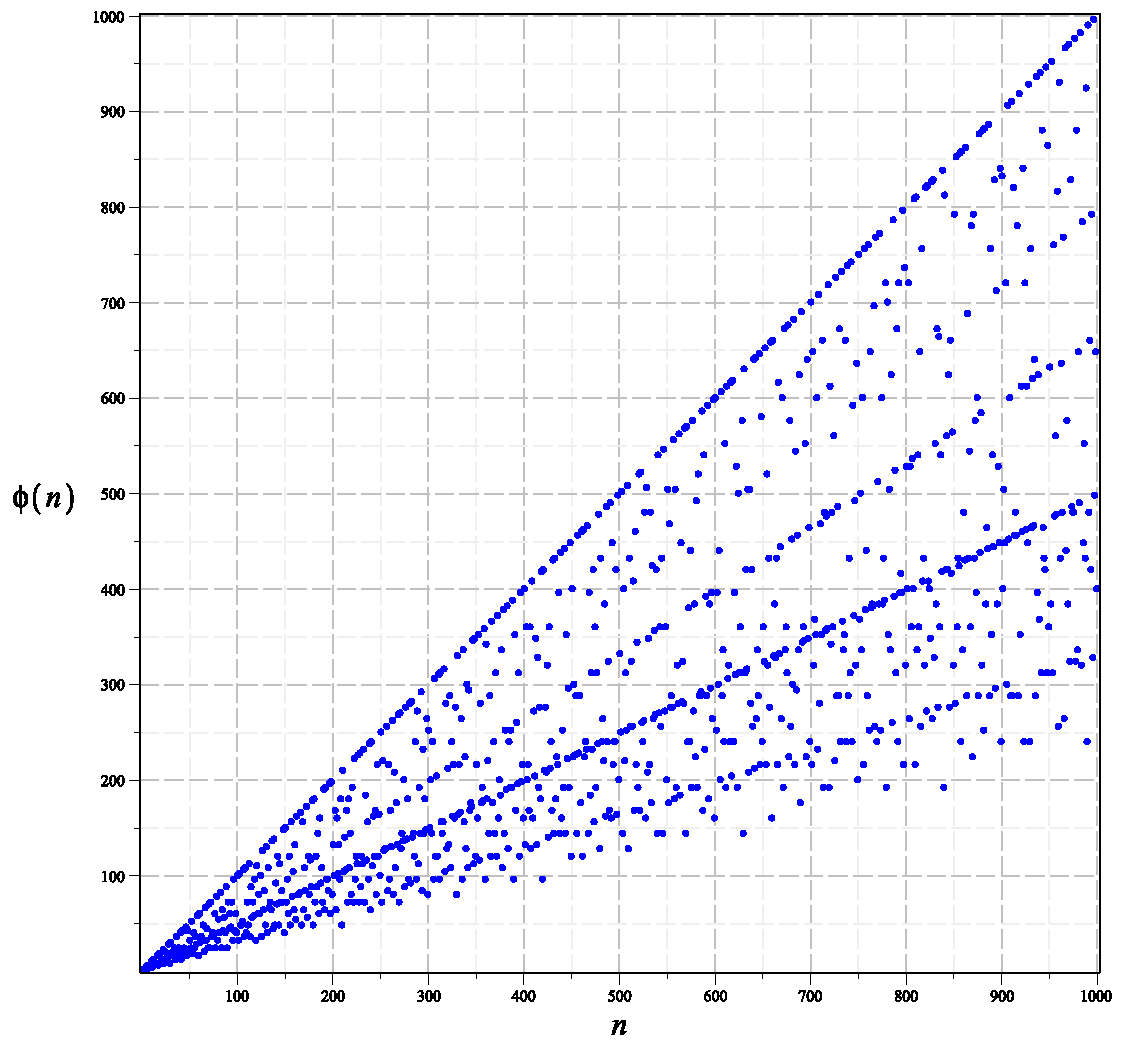
\includegraphics[width=10cm,keepaspectratio]{content/totient.pdf} \\
\vspace*{1cm}
\footnotesize{\url{\homepage}} \\

\vfill
\vspace*{1.5cm}
\begin{flushright}
{\footnotesize Stand: \today}
\end{flushright}
\end{center}
\end{titlepage}							% Titelseite ausgeben
\section*{Vorwort}
\label{sec:preface}
	Der vorliegende Text ist eine Zusammenfassung zur Vorlesung Elementare Zahlentheorie, gelesen von Prof. Dr. Falko Lorenz an der WWU Münster im Wintersemester 2014/2015. Der Inhalt entspricht weitestgehend dem Skript, welches auf der Vorlesungswebsite bereitsgestellt wird, jedoch wird auf Beweise weitestgehend verzichtet. Dieses Werk ist keine Eigenleistung des Autors und wird nicht vom Dozenten der Veranstaltung korrekturgelesen. Für die Korrektheit des Inhalts wird daher keinerlei Garantie übernommen. Bemerkungen, Korrekturen und Ergänzungen kann man folgenderweise loswerden:
	\begin{itemize}
		\item persönlich durch Überreichen von Notizen oder per E-Mail
		\item durch Abändern der entsprechenden TeX-Dateien und Versand per E-Mail an mich
		\item direktes Mitarbeiten via GitHub. Dieses Skript befindet sich im \texttt{latex-wwu}-Repository von Jannes Bantje:
		\begin{center}
			\url{https://github.com/JaMeZ-B/latex-wwu}
		\end{center}
	\end{itemize}

\subsection*{Literatur}
\label{sub:lit}
\begin{itemize}
	\item F. Ischebeck: \href{http://wwwmath.uni-muenster.de/u/ischebeck/}{Einladung zur Zahlentheorie}
	\item R. Remmert, P. Ullrich: \href{http://link.springer.com/book/10.1007/978-3-7643-7731-1}{Elementare Zahlentheorie}
	\item A. Scholz, B. Schöneberg: Einführung in die Zahlentheorie
	\item K. Halupczok: \href{http://wwwmath.uni-muenster.de/u/karin.halupczok/ElZthSS2009Skript.pdf}{Skript zur Elementaren Zahlentheorie}
\end{itemize}

\subsection*{Vorlesungswebsite}
\label{sub:link}
Das vollständige Skript des Dozenten sowie weiteres Material findet man unter folgendem Link:
\begin{center}
	\url{\homepage}
\end{center}

\subsection*{Titelbild}
\label{sub:titlepic}
Plot der Eulerschen $\varphi$-Funktion für $1 \leq n \leq 1000$, erstellt mit Maple. Zugehöriges Maple-Worksheet befindet sich im Git-Repository (siehe oben).

\vfill
\begin{flushright}
	Phil Steinhorst \\
	p.st@wwu.de
\end{flushright}
\newpage
\tableofcontents
\newpage											% Inhaltsverzeichnis ausgeben
\section{Fundamentalsatz der elementaren Arithmetik}
\label{sec:para1}

\minisec{Terminologie}
	Sei $R$ ein kommutativer Ring mit $1 \neq 0$. $R$ heißt \Index{Integritätsring} bzw. \bet{nullteilerfrei}, wenn gilt: \index{Nullteiler} \marginnote{14.10.}
	\[ a \cdot b = 0 \quad \Rightarrow \quad a = 0 \text{ oder } b = 0.\]

\begin{bsp} \label{bsp_integritaetsringe}
	\begin{itemize}
		\item $\ZZ$
		\item $\ZZ[\sqrt{2}] := \{a + b\sqrt{2} : a,b \in \ZZ \} \subseteq \RR$ \\
			$\ZZ[i] := \{a + bi : a,b \in \ZZ\} \subseteq \CC$ \\
			$\ZZ[\sqrt{-5}] := \dots$
		\item $K[X]$ für $K$ Körper \\
			$\ZZ[X]$
		\item $K$ Körper
		\item $\CC \sprod{z} := \penbrace{\text{konvergente Potenzreihen } \sum\limits_{n=0}^{\infty} a_n z^n}$
		\item Nicht nullteilerfrei ist z.B. $\mathcal{C}[0,1] := \{f \colon [0,1] \rightarrow \RR \text{ stetig} \}$
	\end{itemize}
\end{bsp}

\begin{defn}[Teilbarkeit] \label{def_1.1}
	Seien $a,b \in R$. $a$ heißt ein \Index{Teiler} von $b$, wenn ein $q \in R$ existiert mit $b = qa$, und schreiben:
	\[ a | b \]
	Ist $R$ nullteilerfrei und $a \neq 0$, so ist $q$ eindeutig bestimmt.
\end{defn}

\begin{falko}[Triviale Teilbarkeitsregeln] \label{F1.1}
	\begin{enumerate}[(i)]
		\item $a | 0, 1 | a, a | a$
		\item $a | b, b | c \quad \Rightarrow \quad a | c$
		\item $a | b, a | c \quad \Rightarrow \quad a | b+c, a | b-c$
		\item $a_1 | b_1, a_2 | b_2 \quad \Rightarrow \quad a_1 a_2 | b_1 b_2$
		\item $ac | bc \quad \Rightarrow \quad a | b$, falls $c \neq 0$ und $R$ nullteilerfrei.
	\end{enumerate}	
\end{falko}

\begin{defn}[Einheit, assoziiert] \label{def_1.2}
	\begin{enumerate}[(i)]
		\item $e \in R$ heißt eine \Index{Einheit} in $R$, falls $e | 1$ gilt, d.h. falls ein $f \in R$ existiert mit $ef = 1$. $f$ ist eindeutig bestimmt. Wir setzen $e^{-1} := f$ und schreiben auch $\frac{1}{e}$ für $e^{-1}$. \\
		Wir bezeichnen die \Index{Einheitengruppe} von $R$ mit $R^\times := \{x \in R : x \text{ ist Einheit in } R\}$.
		\item $a \in R$ heißt \Index{assoziiert} zu $b \in R$, falls $a | b$ und $b | a$ gilt. Schreibe: $a \assoz b$.
	\end{enumerate}
\end{defn}

\begin{bsp}
	\begin{enumerate}[1)]
		\item Sei $K$ ein Körper, dann ist $K^\times = K \setminus \setnull$. \qquad $\ZZ^\times = \{1,-1\}$, \qquad $K[X]^\times = K^\times$, \\
		$\mathcal{C}[0,1]^\times = \{f \in \mathcal{C}[0,1] : f(x) \neq 0 \text{ für alle } x \in [0,1]\}$, \qquad  $\ZZ[\sqrt{2}]^\times = \{\pm (1+\sqrt{2})^k : k \in \ZZ \}$ \\
		$\ZZ[X]^\times = \{1, -1\}$ \qquad $\CC \sprod{z}^\times = \penbrace*{ \sum a_n z^n \in \CC \sprod{z} : a_0 \neq 0}$
		\item $e \in R^\times \quad \Leftrightarrow \quad e | a$ für jedes $a \in R$.
	\end{enumerate}
\end{bsp}

\begin{falko} \label{F1.2}
	Sei $R$ ein Integritätsring, $a, b \in R$ und $b \neq 0$. Dann gilt:
	\[ a \assoz b \quad \Leftrightarrow \quad \exists e \in R^\times \text{ mit } b = ea \]
\end{falko}

\minisec{Beweis}
	\begin{description}
		\item[\bewrueck] $a | b, e^{-1}b = a, b | a$
		\item[\bewhin] Da $a | b$ und $b | a$, existieren $e, f \in R$, sodass $b = ea$ und $a = fb$. $\Rightarrow b = efb \Rightarrow ef = 1$, da $b \neq 0$ und $R$ nullteilerfrei. \qed
	\end{description}

\setlength{\fboxsep}{10pt}
\setlength{\fboxrule}{3pt}
\begin{center}
	\fbox{\textbf{Ab jetzt ist, wenn nichts anderes gesagt, $R$ ein Integritätsring!}}
\end{center}

\begin{defn}[unzerlegbar, irreduzibel, zusammengesetzt] \label{def_1.3}
	Sei $a \in R \setminus R^\times$. $a$ heißt \Index{unzerlegbar} oder \Index{irreduzibel} in $R$, wenn gilt:
	\[ a = bc \text{ in } R \quad \Rightarrow \quad b \in R^\times \text{ oder } c \in R^\times. \]
	Andernfalls heißt $a$ \bet{zerlegbar}, \bet{zusammengesetzt} oder \bet{reduzibel}.
\end{defn}

\minisec{Bemerkung}
	$a$ unzerlegbar $\quad \Leftrightarrow \quad $ jeder Teiler von $a$ ist Einheit oder assoziiert zu $a$ \\
	$a$ zerlegbar $\quad \Leftrightarrow \quad a$ hat echten Teiler, d.h. einen Teiler, der weder eine Einheit ist noch assoziiert zu $a$

\setcounter{countdef}{2}
\begin{defn}[Primzahl] \label{def_1.3'}
	Ein $p \in \ZZ$ heißt \Index{Primzahl}, wenn $p \in \NN$ und $p$ unzerlegbar in $\ZZ$. Wir beziechnen mit $\PP$ die Menge der Primzahlen von $\ZZ$. $a$ unzerlegbar in $\ZZ \Leftrightarrow a = p$ oder $a = -p$ mit $p \in \PP$.
\end{defn}

\minisec{Bemerkung}
	$a \in \ZZ$ sei zerlegbar, $a \neq 0$. Dann gibt es eine Primzahl $p$ mit $p | a$ und $p \leq \sqrt{|a|}$.

\begin{defn}[Zerlegung in unzerlegbare Faktoren] \label{def_1.4}
	Wir sagen, $a \in R$ besitzt in $R$ eine \Index{Zerlegung in unzerlegbare Faktoren}, wenn
	\begin{equation}
	\begin{aligned}
		a = ep_1p_2\dots p_r \text{ mit } e \in R^\times \text{ und } p_1,\dots,p_r \text{ unzerlegbar} \label{eq_def_1.4}
	\end{aligned}
	\end{equation}
	\eqref{eq_def_1.4} heißt eine Zerlegung von $a$ in unzerlegbare Faktoren. Auch $r = 0$ ist erlaubt.
\end{defn}

\begin{falko} \label{F1.3}
	In $\ZZ$ besitzt jedes $a \neq 0$ eine Zerlegung in unzerlegbare Faktoren.
\end{falko}	

\setcounter{countfalko}{2}
\begin{falko} \label{F1.3'}
	Jede natürliche Zahl $a > 1$ besitzt eine Zerlegung $a = p_1p_2 \dots p_r$ mit Primzahlen $p_1,\dots,p_r$ und $r \geq 1$.
\end{falko}

\minisec{Bemerkung}
	\begin{enumerate}[1)]
		\item Die Aussage F1.3 gilt auch für die Beispiele zu Beginn, mit Ausnahme von $\mathcal{C}[0,1]$.
		\item Sei $R$ ein Integritätsring, der die \Index{Teilbarkeitsbedingung für Hauptideale} erfüllt, so besitzt jedes $a \neq 0$ aus $R$ eine Zerlegung in unzerlegbare Faktoren.
		\item Primzahlen sind die multiplikativen Bausteine (Atome) von $\NN$.
		\item Im Beispiel $\CC\sprod{z}$ von oben gibt es (bis auf Assoziiertheit) nur das einzige unzerlegbare Element $z$. Dieses ist ein \Index{Primelement} (der Begriff folgt weiter unten).
	\end{enumerate}
	
\begin{satz}[Existenz unendlich vieler Primzahlen] \label{satz_1.1}
	Es gibt unendlich viele Primzahlen.
\end{satz}

\textbf{Bemerkungen} \\
	Es sei $p_1,p_2,\dots$ die aufsteigend sortierte Folge der Primzahlen.
	\begin{enumerate}[1)]
		\item $a_n := p_1p_2\dots p_n +1$ ist Primzahl für $n \leq 5$, aber z.B. nicht für $n = 6$. Unklar ist, ob unendlich viele $a_n$ Primzahlen oder keine Primzahlen sind.
		\item Für $x \in \RR_{>0}$ definieren wir:
		\[ \pi(x) := \# \penbrace{p \in \PP : p \leq x}\]
	\end{enumerate}

\minisec{Primzahlsatz (Gauß, Legendre)}
	\begin{equation}
		\pi(x) \sim \frac{x}{\log x}, \text{ d.h. } \lim\limits_{x \rightarrow \infty} \frac{\pi(x)}{x / \log x} = 1 \label{eq_primzahlsatz1}
	\end{equation}
	\begin{equation}
		\pi(x) \sim \int_{2}^{x} \frac{1}{\log t} dt =: \li(x) \label{eq_primzahlsatz_2}
	\end{equation}
	\begin{equation}
	\pi(x) > \frac{x}{\log x} \text{ für alle } x \geq 17 \label{eq_primzahlsatz_3}
	\end{equation}
	\begin{equation}
	\pi(n) > \frac{n}{\log n} \text{ für alle } n \in \NN, n \geq 11 \label{eq_primzahlsatz_4}
	\end{equation}
	
\begin{defn}[eindeutige Zerlegung] \label{def_1.5}
	Sei $R$ ein kommutativer Ring mit $1 \neq 0$. Wir sagen, $a \in R \setminus \setnull$ hat eine \bet{eindeutige} \Index{Zerlegung in unzerlegbare Faktoren}, wenn $a$ eine Zerlegung
	\[ a = ep_1p_2 \dots p_r \]
	in unzerlegbare Faktoren besitzt und eine solche im folgendem Sinne eindeutig ist: Ist auch
	\[ a = e'p_1'p_2'\dots p'_{r'} \]
	eine solche Zerlegung, so gilt $r = r'$ und nach Umnummerierung $p_i' \assoz p_i$ für alle $1 \leq i \leq r$.
\end{defn}

\begin{falko}\label{F1.4}
	In dem Integritätsring $R$ besitze jedes Element $a \neq 0$ eine Zerlegung in unzerlegbare Faktoren. Dann sind äquivalent: \begin{enumerate}[(i)]
		\item Jedes $a \neq 0$ aus $R$ hat eindeutige Zerlegung in unzerlegbare Faktoren.
		\item Ist $p$ unzerlegbar, so gilt: $p | ab \Rightarrow p | a$ oder $p | b$.
	\end{enumerate}
\end{falko}

\begin{defn}[Primelement] \label{def_1.6}
	Sei $R$ ein kommutativer Ring mit $1 \neq 0$. Ein $p \in R\setminus R^\times$ heißt \Index{Primelement} von $R$, wenn für alle $a, b \in R$ gilt:
	\begin{equation}
		p | ab \quad \Leftrightarrow \quad p | a \text{ oder } p | b \label{eq_def_1.6}
	\end{equation}
\end{defn}

\minisec{Bemerkung}
	\begin{enumerate}[1)]
		\item $0$ ist Primelement in $R \Leftrightarrow R$ ist Integritätsring
		\item In einem Integritätsring $R$ gilt: Jedes Primelement $p \neq 0$ ist unzerlegbar.
	\end{enumerate}

\begin{lemma}
	Seien $a, b \in \NN$. Sei $m = \kgV(a,b) \in \NN$. Dann gilt:
	\[ a|c \text{ und } b|c \quad \Rightarrow \quad m | c \]
	$m$ ist also auch minimal bzgl. der Teilbarkeitsrelation $|$.
\end{lemma}

\begin{falko}[Satz von Euklid] \label{F1.5}
	Jede Primzahl $p$ ist ein Primelement von $\ZZ$, d.h. es gilt stets \eqref{eq_def_1.6}. (Das gleiche gilt für $-p$, also für jedes unzerlegbare Element von $\ZZ$.) \index{Satz von Euklid}
\end{falko}

\minisec{Fundamentalsatz der elementaren Arithmetik}
	In $\ZZ$ hat jedes $a \neq 0$ eine eindeutige Zerlegung in unzerlegbare Faktoren. \index{Fundamentalsatz der elementaren Arithmetik}

\minisec{Bemerkung}
	Eindeutige Zerlegung in unzerlegbare Faktoren hat man zum Beispiel auch für die Ringe $\ZZ[\sqrt{2}], \ZZ[i], K[X]$ und $K$ für $K$ Körper, $\ZZ[X]$ und $\CC\sprod{z}$, nicht aber für $\ZZ[\sqrt{-5}]$:
	\[ 3 \cdot 3 = 9 = (2+ \sqrt{-5})(2 - \sqrt{-5}) \]
	Dies sind zwei wesentlich verschiedene Zerlegungen in unzerlegbare Faktoren.

\begin{defn}[Exponent] \label{def_1.7}
	Sei $p$ eine Primzahl und $a \in \ZZ \setminus \setnull$. Dann heißt
	\[ w_p(a) :=\max\{k \in \NN_0 : p^k |a \} \]
	der \Index{Exponent} von $p$ in $a$. Wir setzen $w_p(0) := \infty$.
\end{defn}

\begin{falko}[Eigenschaften der Exponentfunktion] \label{F1.6}
	Die Funktion $w_p \colon \ZZ \rightarrow \NN_0 \cup \{\infty\}$ hat folgende Eigenschaften:
	\begin{enumerate}[(i)]
		\item $w_p(a+b) \geq \min(w_p(a),w_p(b))$ und Gleichheit, falls $w_p(a) \neq w_p(b)$.
		\item $w_p(ab) = w_p(a) + w_p(b)$
	\end{enumerate}
\end{falko}

\begin{satz}[Fundamentalsatz der elementaren Arithmetik] \label{satz_1.2}
	Für jedes $a \in \ZZ \setminus \setnull$ gilt $w_p(a) > 0$ nur für endlich viele $p$. Es ist
	\begin{equation}
		a = \sgn(a) \cdot \prod\limits_p^{} p^{w_p(a)} \label{eq_satz_1.2}
	\end{equation}
\end{satz}

\minisec{Bemerkung}
	\begin{enumerate}[1)]
		\item $w_p$ lässt sich eindeutig zu einer Abbildung $w_p \colon \QQ \rightarrow \ZZ \cup \{\infty\}$ fortsetzen, sodass (ii) für alle $a,b \in \QQ$ gilt. Es gilt dann auch (i). Für $a \in \QQ \setminus \setnull$ ist $w_p(a) \neq 0$ nur für endlich viele $p$, und die Formel \eqref{eq_satz_1.2} gilt entsprechend.  Ferner gilt: $a \in \ZZ \Leftrightarrow w_p(a) \geq 0$ für alle $p$.
		\item Sei
		\[ \NN_0^{(\PP)} := \{ (e_p)_{p \in \PP} : e_p \in \NN_0, e_p = 0 \text{ für fast alle } p \}. \]
		Nach Satz \ref{satz_1.2} sind $(\NN,\cdot)$ und $(\NN_0^{(\PP)},+)$ zwei zueinander isomorphe Halbgruppen. Nach Bemerkung 1) sind $\QQ^\times$ und $\{1,-1\} \times \ZZ^{(\PP)}$ sogar zwei zueinander isomorphe Gruppen.
	\end{enumerate}
	
\begin{defn}[faktorieller Ring, Vertretersystem für Primelemente] \label{def_1.8}
	Ein Integritätsring $R$ heißt \Index{faktoriell}, wenn jedes $a \in R \setminus \setnull$ eine eindeutige Zerlegung in unzerlegbare Faktoren hat. Man spricht dann auch von eindeutiger Primfaktorzerlegung in $R$. \\
	$P$ heißt \bet{Vertretersystem für die Primelemente $\neq 0$} von $R$, wenn:
	\begin{enumerate}[(1)]
		\item Zu jedem Primelement $q \neq 0$ von $R$ gibt es ein $p \in P$ mit $q \assoz p$. 
		\item Für $p, p' \in P$ mit $p \assoz p'$ gilt $p = p'$, d.h. $p$ in (1) ist eindeutig bestimmt durch $q$.
	\end{enumerate}
	Für $R = \ZZ$ nehme man stets $P = \PP$. Für $K$ Körper und $R = K[X]$ nimmt man $P = \{p \in K[X] : p \text{ irreduzibel und normiert}\}$. \index{Primelement} \index{Vertretersystem}
\end{defn}

\begin{falko} \label{F1.7}
	Sei $R$ faktoriell und $P$ ein Vertretersystem für Primelemente. Es gibt zu jedem $p \in P$ eine Funktion $w_p \colon R \rightarrow \NN_0 \cup \{\infty\}$ mit den Eigenschaften (i) und (ii) aus F\ref{F1.6}, sodass gilt: \begin{enumerate}[a)]
		\item Für jedes $a \in R \setminus \setnull$ ist $w_p(a) > 0$ nur für endlich viele $p \in P$.
		\item Für jedes $a \in R \setminus \setnull$ gilt
		\begin{equation}
			a = e \prod\limits_{p \in P}^{} p^{w_p(a)} \label{eq_F1.7}
		\end{equation}
		mit eindeutigem $e \in \RR^\times$.
	\end{enumerate}
\end{falko}

\begin{defn}[ggT und kgV] \label{def_1.9}
	Sei $R$ ein kommutativer Ring mit $1 \neq 0$. Gegeben $a_1, \dots, a_n \in R$.
	\begin{enumerate}[a)]
		\item Ein $d \in R$ heißt ein \Index{größter gemeinsamer Teiler} (ggT) von $a_1,\dots,a_n$, falls:
		\begin{center}
			1. \quad $d | a_i$ für alle $i$ \hspace{3cm} 2. \quad $t | a_i$ für alle $i \Rightarrow t | d$
		\end{center}
		\item Ein $m \in R$ heißt ein \Index{kleinstes gemeinsames Vielfaches} (kgV) von $a_1,\dots,a_n$, falls:
		\begin{center}
			1. \quad $a_i | m$ für alle $i$ \hspace{3cm} 2. \quad $a_i | c$ für alle $i \Rightarrow m | c$
		\end{center}
	\end{enumerate}
\end{defn}

\minisec{Bemerkung}
	\begin{enumerate}[1)]
		\item $d, d'$ ggT von $a_1, \dots, a_n \Rightarrow d \assoz d'$ und $m, m'$ kgV von $a_1, \dots, a_n \Rightarrow m \assoz m'$
		\item Im Allgemeinen ist die Existenz eines ggT und kgV nicht gesichert. In faktoriellen Ringen existieren sie aber immer, siehe dazu folgende Feststellung.
	\end{enumerate}
\newpage
\section{Elliptische Kurven}
\label{sec:para2}
\nextlecture
\subsection{Grundlagen aus der Algebra}
\subsubsection{Polynome}
	Sei $k$ ein beliebiger Körper. \marginnote{[7]}
	
\begin{defn}[Polynom]
	Ein \Index{Polynom} über $k$ in den $n$ Variablen $x_1,\dots,x_n$ ist ein Ausdruck der Form
	\[ f(x_1,\dots,x_n) = \sum\limits_{\nu_1,\dots,\nu_n \geq 0} \alpha_{\nu_1, \dots, \nu_n} x_1^{\nu_1} \cdots x_n^{\nu_n} \]
	mit Koeffizienten $\alpha_{\nu_1,\dots,\nu_n} \in k$, von denen nur endlich viele $\neq 0$ sind. Hat man es mit mehreren Variablen ($n \geq 2$) zu tun, kann man auch kurz
	\[ f(\underline{x}) = \sum_{\uline{\nu} \in \NN_0^n} \alpha_{\uline{\nu}} x_1^{\nu_1} \cdots x_n^{\nu_n} \]
	schreiben, wenn man die Tupelschreibweise $\uline{\nu} \in \NN_0^n$ bzw. $\uline{x} = (x_1, \dots x_n)$ einführt, wobei man für das Monom $x_1^{\nu_1} \cdots x_n^{\nu_n}$ auch kurz $\uline{x}^{\uline{\nu}}$ schreiben kann, wenn klar ist, dass $n \geq 2$ viele Variablen vorliegen. \\
	Die Menge aller Polynome über $k$ in $n$ Variablen wird kurz mit $k[x_1,\dots,x_n]$ oder noch kürzer mit $k[\uline{x}]$ bezeichnet. Wir schreiben dann auch kurz $f \in k[\uline{x}]$, wenn $f(\uline{x})$ ein Polynom ist.
\end{defn}

\begin{bem}
	Durch eine Addition und Multiplikation definiert durch
	\begin{equation}
	\begin{aligned}
		\sum_{\uline{\nu}} \alpha_{\uline{\nu}} \uline{x}^{\uline{\nu}} + \sum_{\uline{\nu}} \beta_{\uline{\nu}} \uline{x}^{\uline{\nu}} &:= \sum_{\uline{\nu}} (\alpha_{\uline{\nu}} + \beta_{\uline{\nu}}) \uline{x}^{\uline{\nu}} \\
		\enbrace*{\sum_{\uline{\nu}} \alpha_{\uline{\nu}} \uline{x}^{\uline{\nu}}} \cdot \enbrace*{\sum_{\uline{\mu}} \beta_{\uline{\mu}} \uline{x}^{\uline{\mu}}} &:= \sum_{\uline{\nu},\uline{\mu}} \alpha_{\uline{\nu}} \beta_{\uline{\mu}} \uline{x}^{\uline{\nu} + \uline{\mu}}
	\end{aligned}
	\end{equation}
	wird $k[\uline{x}]$ zu einem kommutativen Ring mit Eins; das Nullpolynom $0 := \sum_{\uline{\nu}} 0 \uline{x}^{\uline{\nu}}$ ist dabei das Nullelement, das Polynom $1 := 1 \cdot \uline{x}^{\uline{0}} + \sum_{\uline{\nu} \neq 0} 0 \uline{x}^{\uline{\nu}}$ ist das Einselement. \marginnote{"Einspolynom"} \\
	Der Ring $(k[\uline{x}],+,\cdot)$ heißt \Index{Polynomring} über $k$.
\end{bem}

\begin{defn}[Formale Ableitung]
	Für $f(\uline{x}) = \sum_{\uline{\nu}} \alpha_{\uline{\nu}} \uline{x}^{\uline{\nu}} \in k[\uline{x}]$ und $1 \leq j \leq n$ heißt
	\[ \frac{\der f}{\der x_j}(\uline{x}) := \sum_{\uline{\nu}, \nu_j > 0} \alpha_{\uline{\nu}} v_j x_1^{\nu_1} \cdots x_j^{\nu_j-1} \cdots x_n^{\nu_n} \in k[\uline{x}] \]
	die \Index{formale Ableitung} von $f$ nach $x_j$.
\end{defn}

\begin{satz}[Produktregel, Kettenregel]
\label{satz_7.4}
	Für alle $f,g \in k[\uline{x}]$ und $\gamma \in k$ gelten die Ableitungsregeln
	\[ \frac{\der(\gamma f)}{\der x_j} = \gamma \frac{\der f}{\der x_j} \hspace{2cm} \frac{\der(f+g)}{\der x_j} = \frac{\der f}{\der x_j} + \frac{\der g}{\der x_j} \hspace{2cm} \frac{\der(fg)}{\der x_j} = f \frac{\der g}{\der x_j} + g \frac{\der f}{\der x_j} \]
	und für $f \in k[x_1, \dots,x_m], g_1,\dots, g_m \in k[x_1,\dots, x_n]$
	\[ \frac{\der f(g_1,\dots, g_m)}{\der x_j}(\uline{x}) = \frac{\der f}{\der x_1} (g_1,\dots,g_m) \frac{dg_1}{dx_j}(\uline{x}) + \dots + \frac{\der f}{\der x_m} (g_1,\dots,g_m) \frac{\der g_m}{\der x_j}(\uline{x}). \]
\end{satz}

Polynome in einer Variablen $f \in k[x]$ der Form $f(x) = \sum_{\nu = 0}^{k} \alpha_\nu x^\nu$ sind aus den Grundvorlesungen bekannt.
\begin{defn}[Grad]
	Ist $f \neq 0$, so heißt $\deg(f) := \min\{j \in \NN_0 : a_j \neq 0\}$ der Grad von $f$. Für $f \in k[\uline{x}]$ in $n$ Variablen ist $\deg(f) := \min\{\nu_1 + \dots + \nu_n : a_{\uline{\nu}} \neq 0\}$ der \Index{Grad} von $f$. Neu ist bei uns, dass wir uns hier vor allem mit $n = 2$ oder $n = 3$ Variablen beschäftigen werden, wo wir dann auch $f(x,y)$ oder $f(x,y,z)$ schreiben möchten, zum Beispiel $f(x,y) = \alpha_{(2,0)} x^2 + \alpha_{(1,1)} xy + \alpha_{(0,1)}y$. Wir werden dann für die Koeffizienten einfachere Notationen wählen.
\end{defn}

\begin{bem}
	Bleiben wir zunächst beim Polynomring $k[x]$ in einer Variablen $x$. Sei $f \in k[x]$. Wie im Ring $\ZZ$ können wir Teilbarkeit in $k[x]$ studieren und Divisionen mit Rest durchführen (Polynomdivision), daher kann man wie in $\ZZ$ zum Beispiel den ggT von Polynomen mit dem euklidischen Algorithmus ausrechnen. Dies ist aus den Grundvorlesungen bekannt, wir erinnern hier nur an folgendes:
\end{bem}

\begin{defn}[Nullstelle]
	Gegeben sei die Einsetzabbildung
	\begin{equation}
	\begin{aligned}
		k &\longrightarrow k \\
		c &\longmapsto f(c) := \sum_{\nu = 0}^{k} \alpha_\nu c^\nu
	\end{aligned}
	\end{equation}
	Ein Element $c \in k$ heißt \Index{Nullstelle} von $f$, falls $f(c) = 0$ in $k$ ist.
\end{defn}

\begin{bem}
	$c \in k$ ist genau dann Nullstelle, wenn $(x-c)$ ein Teiler von $f$ im Polynomring $k[x]$ ist, d.h. falls ein $g \in k[x]$ existiert mit $(x-c) \cdot g = f$.
\end{bem}

\begin{defn}[Ordnung einer Nullstelle]
	Ist $c$ eine Nullstelle von $f \neq 0$, so gibt es ein maximales $k \geq 1$, sodass $(x-c)^k$ ein Teiler von $f$ ist. Die Zahl $k$ heißt \bet{Ordnung der Nullstelle} $c$. Ist $f(c) \neq 0$, definiert man diese "Nullstellen"ordnung als $0$. \index{Ordnung!Nullstelle}
\end{defn}

\begin{defn}[irreduzibel, prim]
	Ein Polynom $f \in k[x]$ vom Grad $\geq 1$ heißt \Index{irreduzibel} (oder \bet{prim}), falls gilt: Ist $f = u \cdot v$ mit $u,v \in k[x]$, dann ist $\deg(u) = 0$ oder $\deg(v) = 0$, das heißt $f$ kann nicht als Produkt zweier Polynome vom Grad $\geq 1$ geschrieben werden. (vgl. den Begriff "Primzahl" bei $\ZZ$; der Satz von der eindeutigen Zerlegung in irreduzible Polynome heißt der \Index{Satz von Gauß}.)
\end{defn}

Wenn wir $\ZZ$ als Vorbild für den Polynomring $k[x]$ nehmen, möchten wir auch das "Modulorechnen" auf $k[x]$ übertragen, um neue Strukturen zu erhalten. Unsere Moduln sind dann Polynome:
\begin{defn}[Kongruenz, Restklassenring (Polynome)]
	Sei $f \in k[x]$. Dann heißen $a \in k[x]$ und $b \in k[x]$ \bet{kongruent modulo $f$},\index{Kongruenz!Polynome} wenn $f \mid (b-a)$, das heißt falls ein $g \in k[x]$ existiert mit $b = a + fg$.\marginnote{"$\kon$" nur für $\ZZ$} Die Restklassen modulo $f$ sind Teilmengen von $k[x]$ der Gestalt $a + f \cdot k[x] := \{a + fg : g \in k[x]\}$ mit $a \in k[x]$. Das Polynom $a \in k[x]$ heißt ein \Index{Repräsentant} der Restklasse. Ist der Modul $f \in k[x]$ klar, möchten wir dafür auch kurz wieder $\uline{\uline{a}}$ schreiben.\marginnote{doppelt unterstreichen!} \\
	Die Menge der Restklassen modulo $f$ bezeichnen wir mit
	\[ k[x] / (f) := \{a + f\cdot k[x] : a \in k[x]\} = \{\uline{\uline{a}} : a \in k[x]\} \]
	und nennen diese den \bet{Restklassenring modulo $f$}, weil diese bezüglich der Definition $\uline{\uline{a}} + \uline{\uline{b}} := \uline{\uline{a+b}}$ (analog für Multiplikation) für Polynome $a,b \in k[x]$ wieder zu einem kommutativen Ring mit $\uline{\uline{1}}$ als Eins wird. \index{Restklasse!Polynom}
\end{defn}

Doch die einfache Frage, wie viele Elemente der Restklassenring hat, hängt unter anderem vom Körper $k$ ab. Im Fall $k = \FF_p$ beantworten wir diese. Klar ist wegen der Teilbarkeit mit Rest im Ring $k[x]$ (d.h. sind $b,f \in k[x]$ und $f \neq 0$, so existieren eindeutige $g,r \in k[x]$ mit $r = 0$ oder $\deg(r) < \deg(f)$,\marginnote{Polynomdivision} sodass $b = f\cdot g + r$ gilt):
\begin{bem}
\label{bem_7.12}
	Für jede Restklasse $\uline{\uline{a}} = a + f \cdot k[x] \in k[x]/(f)$ gibt es genau einen Vertreter $b \in \uline{\uline{a}} = a + f\cdot k[x]$, das heißt $\uline{\uline{b}} = \uline{\uline{a}}$ bzw. $b + f \cdot k[x] = a + f \cdot k[x]$, mit $b = 0$ oder $\deg(b) < \deg(f)$.
\end{bem}

\subsubsection{Endliche Körper}
\label{subsub:2.1.2}
	Sei nun $k = \FF_p$ mit $p$ prim.

\begin{satz}
	Sei $f \in \FF_p[x]$ irreduzibel mit $r := \deg(f)$. Dann ist $\FF_p[x]/(f)$ ein Körper mit $p^r$ Elementen.
\end{satz}

\minisec{Beweis}
	Dass $\FF_p[x]/(f)$ ein Körper ist, ist klar (Inverse findet man mit dem euklidischen Algorithmus). $\FF_p[x]$ hat $p^r$ Elemente, denn jede Restklasse hat genau einen Vertreter
	\[ b = \underbrace{\alpha_0 + \dots + a_{r-1} x^{r-1}}_{p \text{ Möglichkeiten für jedes } \alpha_j} \qed\]
	
\begin{bem}
	Für jedes $r \in \NN$ gibt es (mindestens) ein irreduzibles Polynom $f \in \FF_p[x]$ mit $\deg(f) = r$.
\end{bem}

\begin{bem}
	Es gibt im Wesentlichen (das heißt bis auf Isomorphie) genau einen endlichen Körper mit $p^r$ Elementen, das heißt welches irreduzible $f$ mit $\deg(f) = r$ wir als Modul nehmen, ist für seine Konstruktion (bis auf Isomorphie!) egal. Wir bezeichnen diesen Körper mit $\FF_{p^r}$.
\end{bem}

\begin{bem}
	Jeder Körper mit endlich vielen Elementen ist einer dieser Körper $\FF_{p^r}$ mit $p$ prim und $r \geq 1$. (ohne Beweis, vgl. Vorlesung "Einführung in die Algebra")
\end{bem}

\begin{bem}
	Wegen Bemerkung \ref{bem_7.12} ist nach Wahl eines irreduziblen Polynom $f \in \FF_p[x], \deg(f) = r$ also
	\[\FF_{p^r} = \{ (\alpha_{r-1} x^{r-1} + \dots + \alpha_1 x + \alpha_0) + f \cdot \FF_p[x] : \alpha_i \in \FF_p\},\]
	die Restklassenvertreter $\alpha_{r-1} x^{r-1} + \dots + \alpha_1 x + \alpha_0$ lassen sich auch durch Koeffizienten-$r$-Tupel $(\alpha_{r-1}, \alpha_{r-2}, \dots, \alpha_1, \alpha_0) \in \FF_{p^r}$ darstellen. Will man mit ihnen stellvertretend für die Polynomrestklassen in $\FF_{p^r}$ rechnen, muss man also erst mit den zugehörigen Polynomen über $\FF_p$ rechnen und modulo $f$ reduzieren.
\end{bem}

\begin{bsp}
	Sei $p = 2, r=3$, wir möchten $\FF_8$ konstruieren.\marginnote{Unterstreichungen weggelassen!} Das Polynom $f(x) = x^3 + x + 1$ ist irreduzibel über $\FF_2 = \{0,1\}$, also ist 
	\[ \FF_8 = \FF_2[x]/(f) = \{ (0,0,0), (0,0,1), (0,1,0), (0,1,1), (1,0,0), (1,0,1), (1,1,0), (1,1,1)\}, \]
	und man rechnet zum Beispiel $(0,1,0) \cdot (1,1,1) = (1,0,1)$, weil
	\[ (0x^2 + 1x + 0) \cdot (x^2 + x + 1) = x^3 + x^2 + x = 1 \cdot (x^3 + x + 1) + (x^2 + 1) \]
	in $\FF_2[x]$ gilt (Division mit Rest durch $f$). \begin{itemize}
	\item Bei Wahl des irreduziblen Polynoms $f(x) = x^3 + x^2 + 1$ ergeben sich zwar andere Rechenregeln für die Vektorenmultiplikation, man erhält aber die selbe "Struktur" bei $+,\cdot$ mit entsprechenden Elementen. Stellen Sie als Übung mal die Multiplikations- und Additionstabellen auf, der Einfachheit halber auch erst mal von $\FF_4$.
	\item Streng genommen müsste man zum Beispiel $\uline{\uline{(\uline{1}, \uline{0}, \uline{1})}} = \uline{\uline{x^2 + \uline{1}}}$ für die Elemente von $\FF_8$ schreiben, um die Reduktion modulo $f$ zu verdeutlichen.
	\end{itemize}
\end{bsp}

\begin{bsp}
	Rechnen in $\FF_{5^3} = \FF_{125}$: Haben wir diesen Körper mit dem irreduziblen Polynom $f = x^3 + x + 1 \in \FF_5[x]$ vom Grad $3$ konstruiert,\marginnote{irreduzibel, da keine Nullstelle und Grad 3!} so rechnen wir in $\FF_{5^3}$ zum Beispiel
	\begin{equation}
	\begin{aligned}
		(1,2,4) \cdot (-1,3,0) &= (x^2 + 2x - 1)(-x^2 + 3x) = -x^4 + 3x^3 - 2x^3 + 6x + x^2 -3x \\
		&= -x^4 + x^3 + x^2 + 3x = (x^3+x+1) \cdot (-x+1) + 2x^2+3x+1 = (2,3,1) \modu f
	\end{aligned}
	\end{equation}
\end{bsp}

\begin{bem}
	Es ist $\Char(\FF_{p^r}) = p$, denn es gilt $\uline{1} + \uline{1} + \dots + \uline{1} = \uline{p \cdot 1} = \uline{0}$, und $p$ ist minimal mit dieser Eigenschaft, da prim.
\end{bem}

\begin{defn}[algebraisch abgeschlossen]
	Ein Körper $k$ ist \Index{algebraisch abgeschlossen}, wenn sich jedes Polynom $f \in k[x], \deg(f) > 0$, als Produkt von linearen Polynomen schreiben lässt, das heißt wenn $f(x) = d(x-c_1) \cdots (x-c_m)$ mit $d,c_i \in k$ gilt.
\end{defn}

\begin{bem}
\label{bem_7.22}
	Man kann jeden Körper $k$ in einen algebraisch abgeschlossenen Körper einbetten. Ein bezüglich "$\subseteq$" minimaler heißt algebraischer Abschluss von $k$, dieser ist eindeutig und wird mit $\overline{k}$ bezeichnet. So ist etwa $\overline{\RR} = \CC$. Der algebraische Abschluss $\overline{\FF_p}$ enthält jeden der Körper $\FF_{p^r}, r \geq 1$, und umgekehrt ist jedes Element von $\overline{\FF_p}$ schon in einem dieser Körper $\FF_{p^r}, r \geq 1$, enthalten. (ohne Beweis)
\end{bem}

\nextlecture
\newpage
\subsection{Der affine Raum, affine Kurven und der projektive Raum}
	Wir stellen den zweidimensionalen affinen und projektiven Raum vor,\marginnote{[8]} das heißt die wohlbekannte affine Ebene $k^2 = k \times k$ und ihre Ergänzung zur projektiven Ebene $\PP^2(k)$ durch "unendlich ferne Punkte". Kurven im Affinen, wie zum Beispiel elliptische Kurven werden dann in der projektiven Ebene intergriert, weil es rechentechnisch einfacher und mathematisch natürlicher ist.
	
\subsubsection{Der affine und projektive Raum}
	Sei $k$ ein beliebiger Körper. Wir stellen uns meistens $\RR$ vor, weil wir über geometrische Objekte nachdenken möchten; $k$ ist in den Anwendungen aber meist ein endlicher Körper.

\begin{defn}[zweidimensionaler affiner Raum]
	Den zweidimensionalen $k$-Vektorraum $k^2 = k \times k$ schreiben wir auch als $\aff^2(k) := \{(x_1,x_2) : x_1,x_2 \in k\}$ und nennen ihn den \bet{zweidimensionalen affinen Raum} über $k$ bzw. \bet{affine Ebene} über $k$. \index{affiner Raum}
\end{defn}

\begin{defn}[Gerade]
	Eine \Index{Gerade} in $\aff^2(k)$ ist eine Teilmenge der Form
	\[ g(a,b,c) := \{(x,y) \in \aff^2(k) : ax + by + c = 0\} \subseteq \aff^2(k) \]
	für ein Tripel $(a,b,c) \in k^3$ mit $a,b \neq 0$.
\end{defn}

\begin{bem}
	Zwei verschiedene Geraden in $\aff^2(k)$ schneiden sich in genau einem Punkt, es sei denn, sie sind parallel, das heißt dann haben sie keinen gemeinsamen Punkt in $\aff^2(k)$. Soweit nichts Neues.
\end{bem}

\begin{bem}
	Die Ausnahme, dass in der "Ebene" $k \times k$ Geraden parallel sein können, möchten wir uns beim Rechnen gerne ersparen. Wir ergänzen die Ebene um "unendlich ferne Punkte" und erklären, dass sich zwei parallele Geraden in genau so einem Punkt schneiden. Durch diese Ergänzung wird die affine Ebene zur \bet{projektiven Ebene}. Wie kann das sinnvoll so umgesetzt werden, dass alle Punkte Koordinaten bekommen, mit denen man wie üblich rechnen kann, sodass bei der Schnittpunktberechnung auch die unendlich fernen Punkte erhalten werden können?
	\begin{figure}[h]
		\centering
		\begin{tikzpicture}
			\foreach \x in {0,1,2,3} {
				\draw (-.2,\x) -- (3.2,\x);
				\draw (\x,-.2) -- (\x,3.2);
			}
			\draw[color=blue,very thick] (.5,.2) -- (1.5,.2) -- (1.5,1.2) -- (1,1.9) -- (.5,1.2) -- (.5,.2);
			
			\draw [ultra thick,->] (4,1.5) -- (6,1.5);
		\end{tikzpicture} \hspace{.3cm}
		\begin{tikzpicture}[scale=1.2]
			\draw (-.2,0) -- (3.2,0);
			\draw (.1,.8) -- (2.9,.8);
			\draw (.4,1.4) -- (2.6,1.4);
			\draw (.7,1.9) -- (2.3,1.9);
			
			\draw (-.1,-.1) -- (.9,2.1);
			\draw (.95,-.1) -- (1.3,2.1);
			\draw (2.05,-.1) -- (1.7,2.1);
			\draw (3.1,-.1) -- (2.1,2.1);
			
			\draw [color=blue, very thick] (.55,.15) -- (.78,.9) -- (1.177,1.3) -- (1.5,.9) -- (1.48,.15) -- (.55,.15);
			\draw [thick,->] (1.1,2.0) -- (1.3,2.5);
			\draw [thick,->] (1.9,2.0) -- (1.7,2.5);
			\draw (1.5,2.55) node[above]{$\infty$};
		\end{tikzpicture}
		\caption{Ergänzung des zweidimensionalen affinen Raums zur projektiven Ebene.}
	\end{figure}
\end{bem}

Zwei Parallelen $g(a,1,c)$ und $g(a,1,d)$ sollen sich dann schneiden, auch rechnerisch. Wir lösen das so, dass in unserer neuen "Ebene" eine dritte "Koordinate" $z$ hinzukommt, welche bei diesen Parallelen also $=0$ sein müsste, wie folgt:

\begin{defn}[projektive Ebene]
	Die \Index{projektive Ebene} über $k$ ist die Menge
	\[ \PP^2(k) = \{ [y_1 : y_2 : y_3] : y_i \in k \text{ nicht alle } 0\}\]
	mit der Vereinbarung, dass $[y_1 : y_2 : y_3] = [z_1 : z_2 : z_3]$ genau dann gilt, wenn es ein $\lambda \in k \setminus \setnull$ gibt mit $y_1 = \lambda z_1, y_2 = \lambda z_2$ und $y_3 = \lambda z_3$.
\end{defn}

\begin{defn}[projektive Ebene (formal)]
	$\PP^2(k)$ ist die Menge der Äquivalenzklassen in $k^3$ bezüglich der Äquivalenzrelation
	\[ (y_1,y_2,y_3) \sim (z_1,z_2,z_3) \quad :\Leftrightarrow \quad \exists \lambda \in k \setminus \setnull : y_i = \lambda z_i, i = 1, 2, 3 \]
	das heißt $\PP^2(k) := (k^3 \setminus \{(0,0,0)\} / \sim$. \\
	Wir schreiben $[y_1 : y_2 : y_3]$ für die Äquivalenzklasse, die von $(y_1,y_2,y_3)$ repräsentiert wird und nennen sie einen \bet{projektiven Punkt}. $y_1,y_2,y_3$ nennen wir \bet{projektive Koordinaten} von $[y_1: y_2 : y_3]$.
\end{defn}

\begin{bem}
	Ist $y_3 \neq 0$, gilt $[y_1 : y_2 : y_3] = \benbrace*{\frac{y_1}{y_3} : \frac{y_2}{y_3} : 1}$, das heißt die dritte (oder jede andere Koordinate $\neq 0$) kann dann auf $1$ gebracht ("normiert") werden.
\end{bem}

Einem projektiven Punkt $[x:y:z]$ entspricht in unserem Modell in $k^3$ die Ursprungsgerade $\{(\lambda x, \lambda y, \lambda z) : \lambda \in k\}$. Diese Punkte sind entweder $[x:y:1]$ oder $[x:y:0]$ mit $x,y \in k$ (nicht $[0:0:0]$!). \\
Zum Beispiel durch die Abbildung
\begin{equation}
\begin{aligned}
	\iota\colon \aff^2(k) &\longrightarrow \PP^2(k) \\
	(x,y) &\longmapsto [x:y:1]
\end{aligned}
\end{equation}
kann die affine Ebene in die projektive eingebettet werden (d.h. $\iota$ ist injektiv).
\begin{figure}[h]
	\centering
	\begin{tikzpicture}
		\draw [thick] (.2,-.2) -- (-1,1);
		\draw [thick] (0,-.3) -- (0,1);
		\draw [thick] (-.2,-.2) -- (1,1);
		
		\draw [fill=white] (-1.5,.8) -- (1.5,.8) -- (1.7,1.2) -- (-1.3,1.2) -- (-1.5,.8);
		
		\draw (-1,1) node[fill,circle,inner sep=1pt]{};
		\draw (0,1) node[fill,circle,inner sep=1pt]{};
		\draw (1,1) node[fill,circle,inner sep=1pt]{};
		\draw (0,0) node[fill,circle,inner sep=1pt]{};
		
		\draw [thick, ->] (-1,1) -- (-2,2);
		\draw [thick, ->] (0,1) -- (0,2.2);
		\draw [thick, ->] (1,1) -- (2,2);
		
		\draw (1.7,1) node[align=left,label={right:$\iota(\aff^2(k))$}] {};
		\draw (.1,0) node[right,align=left] {$\leftarrow$ Ursprung};
	\end{tikzpicture}
\end{figure}

\begin{bem}
	Aber $\PP^2(k)$ enthält zusätzlich noch die projektiven Punkte $[x:y:0]$ mit $x,y \in k$ (nicht $x=y=0$). Offenbar ist $\{[x:y:0] : x,y \in k, \text{ nicht } x = y = 0\}$ eine Gerade in $\PP^2(k)$, die wir \Index{unendlich ferne Gerade} $g_\infty$ nennen möchten, denn mit $j \colon k \rightarrow g_\infty, x \mapsto [x:1:0]$ lässt sich $k$ darin einbetten (das heißt $j$ ist injektiv), wobei auffällt, dass $g_\infty \setminus \im(j)$ aus genau den weiteren Punkt $\oh := [1:0:0]$ besteht, das heißt $g_\infty \setminus \im(j) = \{\oh\}$.
\end{bem}

\begin{bem}
	Somit: $\PP^2(k) = \iota(\aff^2(k)) \sqcup \underbrace{\textcolor{green}{j(k)} \sqcup \textcolor{red}{\{\oh\}}}_{=g_\infty}$ \marginnote{disjunkte Vereinigung}
\begin{figure}[h]
\centering
\begin{tikzpicture}[scale=0.8]
	\draw (-1.5,-.5) -- (-2,-1) -- (3,-1) -- (5,1) -- (3.5,1);
	\draw [dashed] (3.5,1) -- (0,1) -- (-1.5,-.5);
	\draw (-3,-.5) -- (2,-.5) -- (4,1.5) -- (-1,1.5) -- (-3,-.5);
	
	
	\draw [very thick] (0,-1.5) -- (0,-1);
	\draw [thick, dashed] (0,-1) -- (0,-.7);
	\draw [thick, dashed] (0,-.5) -- (0,.5);
	\draw [very thick, ->] (0,0.5) -- (0,2.5) node[above] {$z$};
	\draw [thick, dashed] (0,0) -- (2.5,0);
	\draw [very thick, ->] (2.5,0) -- (5,0) node[right] {$x$};
	\draw [thick, dashed] (0,0) -- (1.5,1.5);
	\draw [very thick, ->] (1.5,1.5) -- (2,2) node[anchor=south west] {$y$};
	
	\draw [color=green, thick, dashed] (-.5,.5) -- (3,.5);
	\draw [color=green, thick] (3,.5) -- (4.5,.5);
	
	\draw (1,0) node[fill,circle,inner sep=1pt,color=red]{};
	\draw (1,0) node[color=red,anchor=south west]{$\oh$};
	
	\draw (0,1) node[fill,circle,inner sep=1pt]{};
	\draw (0,1) node [left,align=right] {$[0;0;1]$};
	
	\draw (5,1.2) node[anchor=north west,align=left] {$g_\infty = \textcolor{green}{j(k)} \sqcup \textcolor{red}{\{\oh\}}$};
\end{tikzpicture}
\hspace{1.5cm}
\begin{tikzpicture}[scale=1.2]
	\draw [very thick, color=green] (-.2,1) -- (2.2,1) node[right]{$j(k)$};
	\draw [very thick,->] (-.2,0) -- (2.5,0) node [right] {$x$};
	\draw [very thick,->] (0,-.2) -- (0,2) node [right] {$y$};
	
	\draw (-.1,-.2) -- (.8,1.6);
	\draw (-.2,-.1818) -- (1.4,1.2727);
	\draw (-.2,-.1333) -- (1.8,1.2);
	
	\draw (1,0) node[fill,circle,inner sep=1pt,color=red]{};
	\draw (1,0) node[color=red,anchor=south west]{$\oh$};
	
	\draw (-.2,2.5) node[right,align=left]{Ansicht auf $x$-$y$-Ebene};
\end{tikzpicture}	
\end{figure}
\end{bem}

Die in $\aff^2(k)$ parallelen Geraden $g(a,1,c) = \{(x,y) \in k^2 : ax + y + c = 0\} = \{(x,-ax-c) : x \in k\}$ und $g(a,1,d)$ müssen die projektiven Punkte $[x:-ax-c:1]$ und $[x:-ax-d:1]$ enthalten. \\
Das klappt, wenn die Gleichung $ax + y \{c,d\} = 0$ zu $ax + y + \{c,d\}z = 0$ ergänzt wird. Sie schneiden sich dann im unendlich fernen Punkt $[1 : -a : 0] = \benbrace*{-\frac{1}{a} : 1 : 0}$, welcher die gemeinsame Steigung $-a$ angibt bzw. die gemeinsame "Richtung" $(1,-a)$. Die gemeinsame Richtung $(1,-a)$ wird zum gemeinsamen Schnittpunkt $\benbrace*{-\frac{1}{a} : 1 : 0}$ erklärt.

\begin{defn}[projektive Gerade]
	Eine \Index{projektive Gerade} ist eine Teilmenge von $\PP^2(k)$ der Form
	\[ g(a,b,c) = \{ [x:y:z] : ax+by+cz = 0\} \text{ für } (a,b,c) \in k^3 \setminus \setnull \]
	Man sagt, die "projektive" Gleichung $ax+by+cz = 0$ ist "durch Homogenisierung" aus $ax+by+c = 0$ entstanden: Durch die Ergänzung mit $z$ haben nun alle Summanden $ax,by,cz$ denselben Grad $1$ als Polynom aus $k[x,y,z]$. Dieses Prinzip werden wir für allgemeinere Kurven für den Übergang vom Affinen ins Projektive übernehmen. Projektive Geraden werden uns in der Form von Tangenten dann wiederbegegnen.
\end{defn}

\minisec{Beispiel und Bemerkung}
	Die projektiven Geraden $g(a,1,c),g(a,1,d)$ schneiden sich in $\penbrace*{-\frac{1}{a}:1:0} \in g_\infty$. Durch je zwei verschiedene Punkte des $\PP^2(k)$ führt genau eine projektive Gerade.
	
\subsubsection{Affine Kurven}
\label{subsub:2.2.2}
	Doch zunächst möchten wir im affinen Raum allgemeinere Kurven untersuchen. Dazu benutzen wir Polynome zu ihrer Beschreibung.
	
\begin{defn}[affine Kurve]
	Sei $f \in k[x,y]$ ein Polynom über $k$ in zwei Variablen $x$ und $y$. Wir bezeichnen die Menge der Nullstellen von $f$ in $k \times k = \aff^2(k)$ als
	\[ \cc_f(k) := \{(u,v) \in \aff^2(k) : f(u,v) = 0\}\]
	Jede solche Nullstellenmenge $\cc_f(k)$ nennen wir eine \Index{affine Kurve}. Ist klar, welches Polynom $f$ vorliegt, schreiben wir auch kurz $\cc(k)$ für $\cc_f(k)$. Geraden sind spezielle affine Kurven (zu linearen Polynomen $f(x,y,z) = ax+by+c$).
\end{defn}

\begin{bem}
	Für uns ist interessant, Kurven über verschiedenen Körpern $k$ zu studieren. Der Fall eines endlichen Körpers ist für Anwendungen interessant, weil dann alle Kurven aus nur endlich vielen Punkten bestehen können.
\end{bem}

\begin{bsp}
	Sei $k = \RR$ und $f(x,y) = y-x^3-x$. Die Nullstellenmenge $\cc_f(k)$ besteht dann aus allen Punkten $(x,y) \in k^2$, welche die Gleichung $y = x^3 + x$ erfüllen. Das reelle Schaubild sieht so aus:
	\begin{figure}[h]
	\centering
	\begin{tikzpicture}[scale=.7]
		\draw [->] (-3,0) -- (3,0) node[above] {$x$};
		\draw [->] (0,-3) -- (0,3) node[right] {$y$};
		\draw [domain=-1.2:1.2,smooth,variable=\x,blue] plot ({\x},{\x*\x*\x + \x});
	\end{tikzpicture}
	\caption{Die Menge $\{(x,y) \in \RR^2 : y = x^3 + x\}$.}
	\end{figure}
	\newpage
	Für $k = \FF_5$ können nur wenige Punkte auf der "Kurve" liegen: Die Tabelle
	\begin{center}
	\begin{tabular}{c|c|c|c|c|c}
	$a$ & $0$ & $1$ & $2$ & $3$ & $4$ \\ 
	\hline $a^3$ & $0$ & $1$ & $3$ & $-3$ & $-1$ \\ 
	\hline $a^3+a$ & $0$ & $2$ & $0$ & 0 & $3$
	\end{tabular} 
	\end{center}
	zeigt, dass $\cc_f(\FF_5) = \{ (0,0), (1,2), (2,0), (3,0), (4,3)\}$ ist, und mit $f_0(x,y) = y^2 - x^3 - x$ haben wir $\cc_{f_0}(\FF_5) = \{(0,0),(2,0),(3,0)\}$. \\
	Ist $\tilde{k} \subseteq k$ ein Teilkörper von $k$ (wie zum Beispiell $\QQ \subseteq \RR$), so folgt auch stets $\cc_f(\tilde{k}) \subseteq \cc_f(k)$. Unsere Kurvenpunkte in $\aff(\FF_5)$ finden wir deswegen zum Beispiel in $\aff(\FF_{25})$ wieder.
\end{bsp}

\begin{defn}[Tangente]
	Eine (affine) \Index{Tangente} an eine affine Kurve $\cc_f(k)$ im Punkt $(a,b) \in \cc_f(k)$ ist die Gerade
	\[ t_f(a,b) = \penbrace*{ (x,y) : \frac{\der f}{\der x} (a,b)x + \frac{\der f}{\der y}(a,b)y + d = 0},\]
	falls diese existiert (wir brauchen, dass $\frac{\der f}{\der x}(a,b), \frac{\der f}{\der y}(a,b)$ nicht beide $=0$). Dabei ist $d \in k$ so gewählt, dass $(a,b) \in t_f(a,b)$ gilt.
\end{defn}

\begin{bem}
	Es ist nicht klar, ob Tangenten stets eindeutig existieren. Affine Kurven können sich selbst schneiden oder scharfe "Spitzen" haben. Siehe z.B. Abbildung~\ref{fig:bsp} in Abschnitt~\ref{sec:para0} auf Seite~\pageref{fig:bsp}.
\end{bem}

\begin{defn}[singulärer Punkt]
	Die affine Kurve $\cc_f(k)$ heißt \bet{singulär im Punkt} $(a,b) \in \cc_f(k)$, falls $\frac{\der f}{\der x}(a,b) = \frac{\der f}{\der y}(a,b) = 0$ gilt. \index{singulär}
\end{defn}

\begin{bem}
	Affine Kurven, die in keinem Punkt singulär sind, haben überall eine wohldefinierte Tangente.
\end{bem}

\begin{bem}
	Es kann vorkommen, dass $\cc_f(k)$ gar keine singulären Punkte enthält, wohl aber über einem Erweiterungskörper von $k$, wie etwa $\overline{k}$, dem algebraischen Abschluss über $k$.
\end{bem}

\begin{bsp}
	Für $f(x,y) = y^2 - x^4 - 2x^2 - 1$ hat $\cc_f(\RR)$ keine singulären Punkte: Es ist $\frac{\der f}{\der x}(a,b) = -4a(a^2+1),\linebreak \frac{\der f}{\der y}(a,b) = 2b$. Allerdings sind $(i,0),(-i,0) \in \CC$ singuläre Punkte in $\cc_f(\CC)$, wo $\CC = \overline{\RR}$.
\end{bsp}

\begin{bsp}
	Sei $f(x,y) = y^2 - x^3 - x$ und $k = \FF_p$. Die Ableitungen sind $\frac{\der f}{\der x} (x,y) = -3x^2-1, \frac{\der f}{\der y}(x,y) = 2y$, das heißt die singulären Punkte $(a,b)$ sind die mit $b^2 = a^3 + a$, $-3a^2 = 1, 2b=0$.\begin{itemize}
		\item Für $p \neq 2$ ist $2b = 0$ nur für $b = 0$ richtig, dann ist $0 = a(a^2+1)$ und $3a^2 = -1$. Es folgt $0 = a(3a^2 + 3) = 2a$ und wegen $p \neq 2$ folgt $a = 0$ im Widerspruch zu $3^2=-1$. Also existieren keine singulären Punkte für $p \neq 2$.
		\item Für $p = 2$ ist $\cc_f(\FF_2) = \{(0,0),(1,0)\}$. Es ist $\frac{\der f}{\der x} (1,0) = 0 = \frac{\der f}{\der y}(1,0)$, das heißt $(1,0)$ ist singulärer Punkt.
	\end{itemize}
\end{bsp}

\nextlecture
\newpage
\subsection{Projektive Kurven}
\subsubsection{Homogene Polynome und projektive Kurven}
\label{sub:2.3} \label{subsub:2.3.1}
	Durch Homogenisierung können wir affine Kurven zu projektiven Kurven machen. \marginnote{[9]}
	
\begin{defn}[homogenes Polynom, Homogenisierung]
	Sei $F \in k[X,Y,Z]$ ein Polynom über $k$ in drei Variablen und $F \neq 0$. Dann heißt $F$ \Index{homogen} vom Grad $d$, falls gilt:
	\[ F(X,Y,Z) = \sum_{v_1,v_2,v_3 \geq 0} \alpha_{v_1,v_2,v_3} X^{v_1} Y^{v_2} Z^{v_3} \]
	und $\alpha_{v_1,v_2,v_3} \neq 0 \Rightarrow v_1 + v_2 + v_3 = d$, das heißt wenn alle Monome in $g$ den Grad $d$ haben.
\end{defn}

\begin{bsp}
	$F(X,Y,Z) = aX + bY + cZ$ ($d=1$) oder $F(X,Y,Z) = Y^2Z-X^3-XZ^2$ ($d=3$).
\end{bsp}

\begin{bem}
	Klar ist, dass ein $f \in k[X,Y]$ durch Ergänzung von $Z$-Potenzen zu einem homogenen Polynom $F_f \in k[X,Y,Z]$ gemacht werden kann: Ist $f(x,y) = \sum_{v_1,v_2 \geq 0} \alpha_{v_1,v_2} x^{v_1} y^{v_2}$ vom Grad $d$, so setze 
	\[ F_f(x,y,z) := \sum_{v_1,v_2 \geq 0} \alpha_{v_1,v_2} x^{v_1} y^{v_2} z^{d-v_1-v_2}.\] Man nennt $F_f$ dann die \Index{Homogenisierung} von $f$. Für diese gilt $F_f(x,y,1) = f(x,y)$.
\end{bem}

\begin{lemma}
	Ist $F \in k[X,Y,Z]$ homogen vom Grad $d$, so gilt für alle $\alpha, \beta, \gamma \in k$ und $\lambda \in k \setminus \setnull$:
	\[ F(\alpha,\beta,\gamma) = 0 \Leftrightarrow F(\lambda \alpha, \lambda \beta, \lambda \gamma) = 0\]
\end{lemma}

\minisec{Beweis}
	Nachrechnen zeigt $F(\lambda \alpha, \lambda \beta, \lambda \gamma) = \lambda^d F(\alpha, \beta, \gamma)$, woraus die Behauptung folgt. \qed

\mbox{}\\	
Somit können wir projektive Kurven definieren:
\begin{defn}[projektive ebene Kurve]
	Sei $F \in k[X,Y,Z]$ homogen. Dann bezeichnen wir die Nullstellenmenge mit
	\[ \cc_F(k) := \{[u:v:w] \in \PP^2(k) : g(u,v,w) = 0\}.\]
	Ist $F$ klar, schreiben wir auch einfach $\cc(k)$ für $\cc_F(k)$. Jede solche Nullstellenmenge heißt eine \Index{projektive ebene Kurve}.
\end{defn}

\begin{bsp}
	Die affine Kurve $\cc_f(x,y)$ zu $f(x,y) = y^2-x^3-x$ kann durch Homogenisieren zu $C_{F_f}(x,y,z)$ mit $F_f(x,y,z) = y^2z-x^3-xz^2$ gemacht werden. Die injektive Abbildung $\iota\colon \aff^2(k) \rightarrow \PP^2(k), (x,y) \mapsto [x:y:1]$ bildet $\cc_f(k)$ nach $\cc_{F_f}(k)$ ab. Die projektive Kurve $\cc_{F_f}(k)$ hat aber noch genau einen weiteren Punkt (auf $g_\infty$), nämlich $[0:1:0]$, das heißt $\cc_{F_f}(k) = \iota(\cc_f(k)) \cup \{[0:1:0]\}$.
\end{bsp}

\begin{lemma}
	$\cc_{F_f}(k) \cap \iota(\aff^2(k)) = \iota(\cc_f(k))$ für jede affine Kurve $\cc_f$ und ihre projektive Kurve $\CC_{F_f}$.
\end{lemma}

\minisec{Beweis}
	$[x:y:1] \in \cc_{F_f}(k) \cap \iota(\aff^2(k)) \Leftrightarrow 0 = F_f(x,y,1) = f(x,y) \Leftrightarrow [x:y:1] \in \iota(\cc_f(k))$. \qed
	
\begin{bem}
	\begin{itemize}
		\item Wir werden hier $\iota$ auch weglassen; es ist klar, was gemeint ist.
		\item Anstelle von $\iota$ können auch die Einbettungen $\iota_2(x,y) = [1:x:y], \iota_3(x,y) = [x:1:y]$ betrachtet werden, das Lemma gilt dann entsprechend.
		\item Geht man für eine projektive Kurve $\cc_F(k)$ zu einer dieser Schnitte mit $\aff^2(k)$ über, so sagt man, man "geht zu affinen Koordinaten" über.
	\end{itemize}
\end{bem}

\begin{defn}[singulärer Punkt, nicht-singulär]
	Sei $F \in k[X,Y,Z]$ homogen vom Grad $d$. Die projektive ebene Kurve $\cc_F(k)$ heißt \bet{singulär im Punkt} \linebreak $P=[a:b:c] \in \cc_F(k)$, falls alle Ableitungen von $F$ in $P$ verschwinden, das heißt
	\[ \frac{\der F}{\der X}(a,b,c) = \frac{\der F}{\der Y}(a,b,c) = \frac{\der F}{\der Z}(a,b,c) = 0.\]
	Die Kurve $\cc_f(k)$ heißt \Index{nicht-singulär}, falls $\cc_F(\overline{k})$ keinen singulären Punkt enthält, wobei $\overline{k}$ einen algebraischen Abschluss von $k$ bezeichnet. \index{singulär}
\end{defn}

\begin{bem}
	Diese Definition hängt nicht davon ab, welche projektive Koordinaten $a,b,c$ eines Punktes $P = [a:b:c]$ betrachtet werden. Sie passt auch mit der alten Definition von "singulären Punkt" für affine Kurven zusammen, wie folgendes Lemma zeigt. Nach dem Lemma genügt es dann, singuläre Punkte, die im Affinen liegen, auf Singularität im Affinen zu testen.
\end{bem}

\begin{lemma}
	Sei $F(X,Y,Z) = \sum_{\uline{v} \geq 0} \alpha_{\uline{v}} X^{v_1} Y^{v_2} Z^{v_3}$ homogen vom Grad $d$ und $f(x,y) = \sum_{\substack{v_1,v_2 \\ v_1 + v_2 \leq d}} \alpha_{v_1,v_2,d-v_1-v_2}x^{v_1} y^{v_2} = F(x,y,1)$, das heißt $F = F_f$. Weiter sei $P \in \cc_F(k)$ mit $P = i(\QQ) \in \iota(\aff^2(k))$. Dann gilt: $\cc_F(k)$ singulär in $P \Leftrightarrow \cc_F(k)$ singulär in $Q$.
\end{lemma}

\minisec{Beweis}
	Haben $Q \in \cc_f(k)$, etwa $Q = (a,b)$, dann ist $P = \iota(Q) = [a:b:1]$. Es ist
	\[ \frac{\der F}{\der X}(X,Y,Z) = \sum_{\substack{v_1 > 0 \\ v_2, v_3 \geq 0}} \alpha_{\uline{v}} v_1 X^{v_1-1} Y^{v_2} Z^{v_3}, \]
	also gilt $\frac{\der F}{\der X}(a,b,1) = \frac{\der f}{\der x}(a,b)$ und entsprechend $\frac{\der F}{\der Y}(a,b,1) = \frac{\der f}{\der y}(a,b)$, sowie
	\[ \frac{\der F}{\der Z}(a,b,1) = \sum_{v_i \geq 0} \alpha_{\uline{v}} v_3 a^{v_1} b^{v_2} = \sum_{v_i \geq 0} \alpha_{v_1,v_2,d-v_1-v_2} (d-v_1-v_2) a^{v_1} b^{v_2} = d \cdot f(a,b) - a\frac{\der f}{\der x}(a,b) - b \frac{\der f}{\der y}(a,b). \]
	Durch Vergleich der Ableitungen folgt die Behauptung in beide Richtungen. \qed
	
\begin{defn}[Tangente]
	Sei $\cc_F(k)$ eine projektive ebene Kurve und $P = [a:b:c]$ ein nicht-singulärer Punkt auf $\cc_F(k)$. Die projektive Gerade $\cc_T(k)$ mit $T(X,Y,Z) := \frac{\der F}{\der X}(a,b,c)X  + \frac{\der F}{\der Y}(a,b,c)Y + \frac{\der F}{\der Z}(a,b,c)Z$ heißt \Index{Tangente} in $P$ an $\cc_F(k)$. Wir schreiben $T_P(\cc_F) := \cc_T(k)$ dafür.
\end{defn}

\begin{bem}
	In nicht-singulären Punkten haben projektive ebene Kurven also eine "schöne" Tangente. Die Voraussetzung "nicht-singulär" braucht man, damit nicht alle drei Ableitungen gleichzeitig verschwinden und so eine projektive Gerade definiert werden kann. Bei Übergang zu affinen Koordinaten erhält man wieder die üblichen (affinen) Tangenten, weil wir dann $Z = 1$ setzen.
\end{bem}

\begin{bsp}
	Sei $\Char(k) \neq 2, f(x,y) := y^2 - 2x^2 - 2, F_f(x,y,z) = y^2-2x^2-2z^2$. Dann ist $(1,2) \in \cc_f(k)$,\linebreak $\frac{\der f}{\der x}(1,2) = -4, \frac{\der f}{\der y}(1,2) = 4$, das heißt $(1,2)$ ist nicht-singulär. Die affine Tangende von $\cc_f$ in $Q = (1,2)$ ist $t_Q(\cc_f) = \{(x,y) \in k^2 : -4x + 4y - 4 = 0\}$, die projektive Tangente von $\cc_F$ in $P = [1:2:1] = \iota(Q)$ ist $T_P(\cc_F) = \{[X:Y:Z] \in \PP^2(k) : -4X + 4Y - 4Z = 0\}$.
\end{bsp}

\begin{mot}
	Wir möchten studieren, wie sich ebene Kurven mit Geraden schneiden und die folgenden Fälle unterscheiden können:
	\begin{figure}[h]
	\centering
	\begin{tikzpicture}[scale=.9]
		\draw[scale=2,domain=-1:1.2,smooth,variable=\x,blue] plot ({\x},{1*\x*\x*\x - .5*\x*\x - 1.25*\x});
		\draw[very thick,domain=-1.8:.5,smooth,variable=\x,red] plot ({\x},{\x+.5});
		\draw (0,-2.5) node[align=center]{transversaler Schnitt};
	\end{tikzpicture}
	\hspace{1cm}
	\begin{tikzpicture}[scale=.9]
		\draw[scale=2,domain=-1:1.2,smooth,variable=\x,blue] plot ({\x},{1*\x*\x*\x - .5*\x*\x - 1.25*\x});
		\draw[very thick,domain=-1.8:1.5,smooth,variable=\x,red] plot ({\x},{-0.5*\x + .32});
		\draw (0,-2.5) node[align=center]{einfache Tangente};
	\end{tikzpicture}
	\hspace{1cm}
	\begin{tikzpicture}[scale=.9]
		\draw[scale=2,domain=-1:1.2,smooth,variable=\x,blue] plot ({\x},{1*\x*\x*\x - .5*\x*\x - 1.25*\x});
		\draw[very thick,domain=-1:1.4,smooth,variable=\x,red] plot ({\x},{-1.25*\x});
		\draw (0,-2.5) node[align=center]{Wendepunkt-Tangente};
	\end{tikzpicture}
	\caption{Wendepunkt-Tangenten liefern gute Approximationen an eine Kurve.}
	\end{figure}
\end{mot}

\begin{defn}[Schnittmultiplizität, Vielfachheit]
	Sei $\cc_F(k)$ eine projektive Kurve zum homogenen Polynom $F \in k[X,Y,Z]$, sei $G(\alpha,\beta,\gamma)$ eine projektive Gerade und $P \in G(\alpha,\beta,\gamma)$ ein Punkt. Ist $P$ kein Schnittpunkt von $\cc_F(k)$ und $G$, setzen wir $m(P;G,\cc_F) := 0$. Ansonsten hat das Polynom $\Psi(t) := F(a+ta', b+tb', c+tc') \in k[t]$ eine Nullstelle in $t = 0$, wobei $P = (a,b,c)$ und $P'=(a',b',c') \in G$ sind. Dann sei $m(P;G,\cc_F)$ die Ordnung der Nullstelle $t = 0$ von $\Psi \in k[t]$, falls $\Psi \neq 0$. Die Zahl $m(P;G,\cc_F)$ heißt \Index{Schnittmultiplizität} bzw. \Index{Vielfachheit}, mit der sich $G$ und $\cc_F$ im Punkt $P$ schneiden.
\end{defn}

\begin{bem}
	Es ist $m(P;G,\cc_F)$ unabhängig von der Wahl von $P'$.
\end{bem}

\begin{bsp}
	Sei $f(x,y) = x(x-1)(x-2)-y \in \RR[x,y]$, das heißt $f(x,y) = x^3 - 3x^2 + 2x - y$ und $F(X,Y,Z) = F_f(X,Y,Z) = X^3-3X^2Z + 2XZ^2-YZ^2$.\\
	Da $\frac{\der f}{\der x} = 3x^2 - 6x + 2, \frac{\der f}{\der y} = -1$, hat $\cc_f$ in $(0,0) \in \cc_f$ die affine Tangente $t_{(0,0)}(\cc_f) = \{(x,y) \in \RR^2 : 2x-y = 0\}$, projektiv aufgefasst lautet die Tangente $T_{(0,0)}(\cc_F) = \{[x:y:z] \in \PP^2(\RR) : 2X-Y + 0Z = 0\} = G(2,-1,0)$. Die Gerade $G(2,-1,0)$ schneidet $\cc_F$ in $[3:6:1]$ und in $[0:0:1]$. Dann haben wir $m([3:6:1];G,\cc_F)=1$, weil
	\begin{equation}
	\begin{aligned}
		\Psi(t) &= F(3+t \cdot 0, 6 + t \cdot 0, 1 + t \cdot 1) \\
		&= 3^3 - 3 \cdot 3^2(1+t) + 2 \cdot 3 \cdot (1+t)^2 - 6 \cdot (1+t)^2 \\
		&= 0 \cdot t^2 + (-3^3 + 6 \cdot 2 - 12)t + (3^3 - 3^3 +6 -6) = -3^3 t^1
	\end{aligned}
	\end{equation}
	eine einfache Nullstelle in $t = 0$ hat, sowie $m([0:0:1];G,\cc_F) = 2$, weil
	\[ \widetilde{\Psi}(t) = F(0+3t,0+6t,1+t) = (3t)^3 - 3(3t)^2(1+t)+2(3t)(1+t)^2-(6t)(1+t)^2 = -3^3 t^2.\]
\end{bsp}

\begin{erl}
	Ist $m(P;G,\cc_F) = 1$, liegt ein transversaler Schnitt der Geraden $G$ mit der Kurve $\cc_f$ vor. Ist $m(P;G,\cc_F) = 2$, so ist $G$ eine "einfache" Tangente an $\cc_F$. Falls $m(P;G,\cc_F) \geq 3$, ist die Tangente eine sehr gute Approximation an $\cc_F$ von "Ordnung $\geq 3$" (da die Schnittmultiplizität genau die Nullstellenordnung von $\Psi(t)$ in $t = 0$ ist).
\end{erl}

\begin{bem}
\label{bem_9.20}
	Ist der Körper $k$ algebraisch abgeschlossen, zerfällt $\Psi$ fast vollständig in Linearfaktoren. Es folgt, dass dann die Summe der Schnittmultiplizitäten aller Schnittpunkte von $G$ mit $\cc_F$ genau $\deg(\Psi) = \deg(F)$ ist, das heißt $\sum_{P \in G \cap \cc_F} m(P;G,\cc_F) = \deg(F)$. Ist $k$ ein beliebiger Körper, so folgt
	\[ \sum_{P \in G \cap \cc_F} m(P;G,\cc_F) \leq \deg(F).\]
\end{bem}

\begin{bem}
	Alle diese Ergebnisse gelten nicht, wenn das lineare Polynom, welches $G$ erklärt, ein Teiler des Polynoms $F$ ist, denn dann lassen sich keine Schnittmultiplizitäten erklären: Ist $G = G(\alpha,\beta,\gamma)$ durch $\alpha X + \beta Y + \gamma Z = 0$ erklärt und $F(X,Y,Z) = (\alpha X + \beta Y + \gamma Z) \cdot H(X,Y,Z)$ für ein $H \in k[X,Y,Z]$, so folgt $G \subseteq \cc_F$ und für $[a:b:c],[a' : b' : c'] \in G$ ist dann
	\[ \Psi(t) = F(a+ta', b+tb',c+tc') = (a(a+ta')+\beta(b+tb') + \gamma(c+tc')) \cdot H(\dots) = 0 \cdot H(\dots) = 0 \]
	das Nullpolynom, also die Nullstellenordnung von $t = 0$ nicht definiert.
\end{bem}

Wir zeigen nun, dass wir bei Tangenten in einem Kurvenpunkt immer die Schnittmultiplizität $\geq 2$ haben, sofern der Grad der Kurve auch $\geq 2$ ist.
\begin{satz}
\label{satz_9.22}
	Sei $P \in \PP^2(k)$ ein nicht-singulärer Punkt auf $\cc_F$, wobei $\deg(F) \geq 2$ sei, und $T = T_P(\cc_F)$ die Tangente an $\cc_F$ im Punkt $P$. Dann ist $m(P;T,\cc_F) \geq 2$.
\end{satz}

\minisec{Beweis}
	Sei $T = F(\alpha,\beta,\gamma) = \{[X:Y:Z] : \alpha X + \beta Y + \gamma Z = 0\}$ die Tangente in $P = [a:b:c] \in G \cap \cc_F$, also $\alpha = \frac{\der F}{\der X}(a,b,c), \beta = \frac{\der F}{\der Y}(a,b,c), \gamma = \frac{\der F}{\der Z}(a,b,c)$. Sei $Q = [a',b',c'] \in G$ ein beliebiger weiterer Punkt auf $G$, und $\Psi(t) = F(a+ta',b+tb',c+tc')$. Dann ist $\Psi(0) = 0$, da $P \in \cc_F$, und laut Kettenregel (vgl. Satz~\ref{satz_7.4}) ist
	\[ \Psi'(0) = \frac{\der F}{\der X}(a,b,c) \cdot a' + \frac{\der F}{\der Y}(a,b,c) \cdot b' + \frac{\der F}{\der Z}(a,b,c) \cdot c' = \alpha a' + \beta b' + \gamma c' = 0, \]
	weil $Q \in G$. Mit $\Psi(0) = 0, \Psi'(0)=0$ folgt $m(P;T;\cc_F) \geq 2$. \qed

\nextlecture	
\subsubsection{Der Satz von Bézout}
\label{subsub:2.3.2}
	Wir zeigen in diesem Abschnitt, dass Kurven im Allgemeinen nicht allzu viele Schnittpunkte haben: \marginnote{[10]}

\begin{satz}[Satz von Bézout]
\label{satz_10.1}
	Zwei Kurven $\cc_{F_1}, \cc_{F_2}$ in $\PP^2(k)$ können sich in nicht mehr als $\deg(F_1) \cdot \deg(F_2)$ vielen Schnittpunkten treffen, es sei denn, $F_1$ und $F_2$ haben einen gemeinsamen Teiler vom Grad $\geq 1$. Das heißt: \index{Satz von Bézout}
	\[ \ggT(F_1,F_2) = 1 \Rightarrow \#(\cc_{F_1} \cap \cc_{F_2}) \leq \deg(F_1) \cdot \deg(F_2) \]
\end{satz}

\begin{bem}
	Dieser Satz ist eine sehr schwache Form des Satzes von Bézout, welcher besagt: \\
	Sei $k$ ein algebraisch abgeschlossener Körper und seien $F_1,F_2 \in k[X,Y,Z]$ zwei homogene Polynome mit $\ggT(F_1,F_2) = 1$, die zwei ebene projektive Kurven $\cc_{F_1}$ und $\cc_{F_2}$ definieren. Dann ist
	\[ \sum_{P \in \cc_{F_1} \cap \cc_{F_2}} m(P;\cc_{F_1},\cc_{F_2}) = \deg(F_1) \cdot \deg(F_2). \]
	Ist $k$ ein beliebiger Körper, gilt dies mit "$\leq$" statt "$=$".
\end{bem}

\begin{bem}
	\begin{itemize}
		\item Zum Beweis dieses allgemeinen Bézout-Satzes werden mehr Mittel aus der algebraischen Geometrie benötigt, als wir hier zeigen können. Für unsere Zwecke, das Studium elliptischer Kurven, reicht die schwache Version aus Satz~\ref{satz_10.1}, die wir hier beweisen, und insbesondere die spezielle Verschärfung aus Satz~\ref{satz_10.15}.
		\item Die Kurven können singuläre Punkte enthalten.
		\item Den Fall $\deg(F_1) = 1$, das heißt wenn $F_1$ eine Gerade $\cc_{F_1}$ erklärt, haben wir bereits in Bemerkung~\ref{bem_9.20} gezeigt.
		\item Den Begriff der Schnittmultiplizität müsste man für Schnittpunkte zweier beliebiger ebener Kurven verallgemeinern. Wir verzichten hier darauf.
		\item Aus diesem (allgemeinen) Satz von Bézout folgt bereits die schwache Version aus Satz~\ref{satz_10.1}, denn für Schnittpunkte ist $m(P;\cc_{F_1},\cc_{F_2}) \geq 1$, also ist
		\[ \#(\cc_{F_1} \cap \cc_{F_2}) = \sum_{P \in \cc_{F_1} \cap \cc_{F_2}} 1 = \sum_{P \in \cc_{F_1} \cap \cc_{F_2}} m(P;\cc_{F_1},\cc_{F_2}) \leq \deg(F_1) \cdot \deg(F_2).\]
	\end{itemize}
\end{bem}

\begin{bsp}
	Gegeben seien die Parabeln $F_1(X,Y,Z) = X^2 - 3XZ+Z^2-YZ$ und $F_2(X,Y,Z) = -X^2 + 3XZ - 3Z^2 - YZ$ mit den beiden affinen reellen Schnittpunkten $[1:-1:1]$ und $[2:-1:1]$. Laut Bézout-Satz haben die Parabeln noch zwei weitere Schnittpunkte über $\CC$. Diese sind nicht im Affinen, weil die Gleichung $F_1(X,Y,1) = F_2(X,Y,1)$ genau die Lösungen $(1,-1),(2,-1)$ hat. Mit der Gleichung $F_1(X,Y,0) = F_2(X,Y,0) \Leftrightarrow X^2 = -X^2$ erhält man $X = 0$, also den (unendlich fernen) Punkt $[0:1:0] =: \oh$ als einzigen projektiven Schnittpunkt. Eine genaue Analyse würde zeigen, dass $\oh$ die Schnittmultiplizität $2$ hat.
\end{bsp}

\begin{defn}[Resultante]
\label{def_10.5}
	Seien $f,g \in k[X]$ Polynome vom Grad $m = \deg(f), n=\deg(g)$, etwa gegeben durch
	\begin{equation}
	\begin{aligned}
		f &= a_mX^m + a_{m-1}X^{m-1} + \dots + a_1X + a_0 \\
		g &= b_nX^n + b_{n-1}X^{n-1} + \dots + b_1X + b_0
	\end{aligned}
	\end{equation}
	Sei
	\[ M(f,g) := \begin{pmatrix}
	a_0 &  &  &  & b_0 &  &  &  \\ 
	a_1 & a_0 &  &  & b_1 & b_0 &  &  \\ 
	\vdots & a_1 & \ddots &  & \vdots & b_1 & \ddots &  \\ 
	a_m & \vdots & \ddots & a_0 & b_n & \vdots & \ddots & b_0 \\ 
	 & a_m &  & a_1 &  & b_n &  & b_1 \\ 
	 &  & \ddots & \vdots &  &  & \ddots & \vdots \\ 
	 &  &  & a_m &  &  &  & b_n
	\end{pmatrix} \in k^{(m+n) \times (m+n)},\]
	das heißt $M(f,g)$ besteht aus $n$ Spalten mit den Koeffizienten von $f$ und $m$ Spalten mit den Koeffizienten von $g$. Dann heißt $\Res(f,g) = \det(M(f,g)) \in k$ die \Index{Resultante} von $f$ und $g$.
\end{defn}

\begin{bem}
\label{bem_10.6}
	\begin{itemize}
		\item Anstelle von $k$ können auch beliebige kommutative Ringe mit $1$ in der Definition stehen.
		\item $\Res(f,g)$ kann als Polynom in den Unbestimmten $a_0,\dots,a_m, b_0, \dots, b_n$ angesehen werden. Für einen darin vorkommenden Term $\prod_{i,j} a_i^{\nu_i} b_j^{\mu_j}$ gilt $\sum_{i=0}^{m} v_i (m-i) + \sum_{j=0}^{n} \mu_j (n-j) = mn$. (ohne Beweis)
	\end{itemize}
\end{bem}

\begin{bsp}
	Sei $k = \RR$, $f(x) = x^2+2x-1$, $g(x) = 4x^3 - 3x + 5$. Dann ist
	\[
		M(f,g) = \begin{pmatrix}
		-1 & 0 & 0 & 5 & 0 \\ 
		2 & -1 & 0 & -3 & 5 \\ 
		1 & 2 & -1 & 0 & -3 \\ 
		0 & 1 & 2 & 4 & 0 \\ 
		0 & 0 & 1 & 0 & 4
		\end{pmatrix} 
	\]
\end{bsp}

\begin{satz}
\label{satz_10.8}
	Sei $S$ ein faktorieller Ring (z.B. Polynomring oder ein Körper), $f,g \in S[X]$ Polynome mit $\deg(f)=m, \deg(g)=n$. Dann sind äquivalent: \begin{enumerate}[(i)]
		\item $f,g, \in S[X]$ haben einen gemeinsamen nichtkonstanten Teiler in $S[X]$
		\item Es gibt $f_0,g_0 \in S[X] \setminus \setnull$ mit $\deg(f_0) \leq m-1, \deg(g_0) \leq n-1$ und $f_0 g= g_0 f$
		\item $\Res(f,g) = 0$
	\end{enumerate}
\end{satz}

\minisec{Beweis}
	\begin{description}
		\item[(i)$\Rightarrow$(ii):] Sei $h$ ein gemeinsamer Teiler, $\deg(h) \geq 1$. Dann setze $f_0 = \frac{f}{h}, g_0 = \frac{g}{h}$.
		\item[(i)$\Leftarrow$(ii):] Sind $f_0,g_0$ wie in (ii) und $h = \ggT(f,g)$, folgt $\ggT\enbrace*{\frac{f}{h},\frac{g}{h}}=1$. Nach Voraussetzung ist $\frac{f}{h} \cdot g_0 = f_0 \cdot \frac{g}{h}$, also ist $\frac{f}{h} \mid f_0$, das heißt $\deg\enbrace*{\frac{f}{h}} \leq \deg(f_0) \leq m-1$, also $\deg(h) \geq 1$.
		\item[(ii)$\Leftrightarrow$(iii):] $f_0, g_0$ entsprechen den nichttrivialen Lösungen des linearen Gleichungssystems
		\[ \sum_{k=1}^{n} c_k T^{k-1} f + \sum_{k=1}^m c_{n+k} T^{k-1} g = 0. \]
		Bezüglich der Basis $T^0, T^1, \dots, T^{n+m-1}$ über $S$ wird das LGS gerade durch $M(f,g)$ beschrieben. \qed
	\end{description}
	
\begin{bew}[von Satz~\ref{satz_10.1}]
	Wir nehmen zum Beweis ohne Einschränkung an, dass $k$ ein unendlicher Körper ist, andernfalls können wir zum Beispiel zum algebraischen Abschluss $\overline{k}$ übergehen, der jedenfalls unendlich ist, vergleiche dazu Bemerkung~\ref{bem_7.22}; denn für eine Körpererweiterung könnte es mehr Schnittpunkte geben. Sei $d_1 = \deg(F_1)$ und $d_2 = \deg(F_2)$. \\
	Angenommen, $\cc_{F_1}$ und $\cc_{F_2}$ hätten mindestens $d_1 d_2+1$ viele Punkte gemeinsam (wir zeigen, dass dann\linebreak $\deg(\ggT(F_1,F_2)) \geq 1$ sein müsste). Seien $P_0, P_1, \dots, P_{d_1d_2}$ Schnittpunkte von $\cc_{F_1}$ und $\cc_{F_2}$.
\end{bew}

\begin{bew}[Fortsetzung]
	Wir können ohne Einschränkung annehmen, dass die Punkte $P_i = (x_i,y_i), i=0,\dots,d_1d_2$, verschiedene\linebreak $x$-Koordinaten und verschiedene $y$-Koordinaten haben (sonst erreicht man dies wieder durch eine Verschiebung bzw. lineare Transformation, da $k$ unendlich ist).
\end{bew}

\begin{bew}[Fortsetzung]
	Wir können eine Gerade $G(\alpha,\beta,\gamma) = \{ [x:y:z] \in \PP^2(k) : \alpha x + \beta y + \gamma z = 0\}$ finden, die durch keine dieser Punkte $P_0, \dots, P_{d_1d_2}$ geht, weil $k$ unendlich ist. Diese Gerade sei ohne Einschränkung $g_\infty$, die unendlich ferne Gerade (durch eine Verschiebung bzw. lineare Transformation lässt sich dies erreichen).
\end{bew}

\begin{bew}[Fortsetzung]
	Somit ist das Problem auf ein affines Problem zurückgeführt worden. Die zugehörigen affinen Kurven seien durch $f_1,f_2 \in k[x,y]$ gegeben, das heißt $f_1(x,y) := F_1(X,Y,1), f_2(x,y) := F_2(X,Y,1)$, mit $\deg(f_1) \leq d_1$,\linebreak $\deg(f_2) \leq d_2$. Wir können ohne Einschränkung sogar $\deg(f_1) = d_1$, $\deg(f_2) = d_2$ annehmen (nach geeigneter Transformation der Koordinaten der Art $X \rightarrow X + \varepsilon Y, Y \rightarrow Y$ ergeben sich für $F_1(X,Y,0) = \sum_{i+j = d_1} c_{ij} X^i Y^j$,\linebreak $F_2(X,Y,0) = \sum_{i+j = d_2} d_{ij} X^i Y^j$ die Terme $(\sum_{i+j = d_1} c_{ij} \varepsilon^i) Y^{d_1}$ in $\widetilde{F_1}(X,Y,0)$ und $(\sum_{i+j=d_2} d_{ij} \varepsilon^i)Y^{d_2}$ in $\widetilde{F_2}(X,Y,0)$).
\end{bew}

\begin{bew}[Fortsetzung]
	Wir betrachten $f_1,f_2 \in (k[x])[y]$ als Polynome in $y$ mit Koeffizienten in $k[x]$ und berechnen die Resultante $R(f_1,f_2) \in k[x]$, diese hat den Grad $d_1 d_2$ in $x$ nach Bemerkung~\ref{bem_10.6}. Sei $R(x) := R(f_1,f_2) \in k[x]$.
\end{bew}

\begin{bew}[Fortsetzung]
	Für jedes $x_i$ haben die Polynome $f_1(x_i,y), f_2(x_i,y) \in k[y]$ eine Faktor $y-y_i \in k[y]$ gemeinsam. Für die $x = x_i$ muss $R(x)$ also verschwinden: $R(x_i) = 0, i=0, \dots, d_1d_2$. Also hat $R(x)$ mehr Nullstellen ($d_1d_2+1$ viele) als sein Grad $d_1d_2$, $R(x)$ muss also das Nullpolynom (in $x$) sein. Aber dann haben $f_1,f_2 \in (k[x])[y]$ einen gemeinsamen Teiler vom Grad $\geq 1$ wegen Satz~\ref{satz_10.8}, (iii) $\Rightarrow$ (i). \qed
\end{bew}

\begin{satz}
\label{satz_10.15}
	Sei $k$ ein beliebiger Körper, $F_1,F_2 \in k[X,Y,Z]$ homogene Polynome mit $d_1 = \deg(F_1), d_2 = \deg(F_2)$ und $\ggT(F_1,F_2) = 1$, und es seien $d_1d_2 - 1$ viele Schnittpunkte von $\cc_{F_1}$ und $\cc_{F_2}$ gegeben. Dann haben sie einen weiteren Schnittpunkt in $\PP^2(k)$ gemeinsam.
\end{satz}

\minisec{Beweis}
	Wir im Beweis von Satz~\ref{satz_10.1} von Bézout erhalten wir ein Polynom $R(x) \in k[x]$ vom Grad $=d_1d_2$. Es hat $d_1d_2-1$ viele Nullstellen $x_1, \dots, x_{d_1 d_2-1}$ laut Voraussetzung, ist also durch $(x-x_1) \cdots (x-x_{d_1d_2-1})$ teilbar, der Quotient ist vom Grad $1$, also $=r \cdot (x-a) \in k[x]$ mit einer (weiteren) Nullstelle $a \in k$.\\
	Somit haben $f_1(a,y), f_2(a,y) \in k[y]$ einen gemeinsamen Faktor vom Grad $\geq 1$. Dieser Grad ist $1$ (denn wäre er $\geq 2$, würde er über $\overline{k}$ in mindestens zwei Linearfaktoren zerfallen, die dann zu zwei weiteren Schnittpunkten mit gleicher $x$-Koordinate $a$ führen würden, sodass es $\geq (d_1d_2-1)+2 > d_1d_2$ viele Schnittpunkte geben müsste -- im Widerspruch zu Satz~\ref{satz_10.1}). Also gibt es nur noch genau einen weiteren Schnittpunkt $(a,y)$ von $\cc_{F_1}$ und $\cc_{F_2}$. \qed
	
\begin{bsp}
\label{bsp_10.16}
	Sei $k$ ein beliebiger Körper, $F_1,F_2 \in k[X,Y,Z]$ homogen, $\deg(\ggT(F_1,F_2)) = 0$, und sei $\deg(F_1) = 1, \deg(F_2) = 3$. Dann ist $\sum_{P \in \cc_{F_1} \cap \cc_{F_2}} m(P;\cc_{F_1},\cc_{F_2}) \in \{0,1,3\}$.
\end{bsp}
	
\nextlecture
\newpage
\subsection{Elliptische Kurven}
\subsubsection{Definition elliptischer Kurven und vereinfachte Weierstraßgleichungen}
	Wir geben nun die Definition einer elliptischen Kurve. Sei $k$ ein Körper. \marginnote{[11]}
	
\begin{defn}[elliptische Kurve]
	Eine \Index{elliptische Kurve} $E(k)$ ist eine nicht-singuläre, irreduzible projektive Kurve vom Grad $3$, die einen (rationalen) Wendepunkt enthält.
\end{defn}
	
\begin{bem}
	\begin{itemize}
		\item Es reicht, die Wendepunktbedingung durch $E(k) \cap \PP^2(\QQ) \neq \emptyset$ zu ersetzen (ist aber aufwendig zu zeigen, lassen dies deswegen sein).
		\item Eine Kurve $\cc$ heißt \bet{irreduzibel}, wenn sie nicht die Vereinigung zweier Kurven $\neq \cc$ ist, z.B. ist $\cc_F(k)$ mit $F(X,Y,Z) = XY$ reduzibel. \index{irreduzibel!Kurve}
	\end{itemize}
\end{bem}

\begin{bem}
	Durch eine so genannte \Index{birationale Transformation} kann angenommen werden, dass der Wendepunkt ohne Einschränkung $\oh := [0:1:0]$ ist. Eine Übungsaufgabe zeigt, dass dann die Kurvengleichung die folgende vereinfachte Form hat:
\end{bem}

\begin{defn}[elliptische Kurve (lange Weierstraßform)]
	Eine \Index{elliptische Kurve} $E_F(k)$ ist eine nicht-singuläre, projektive ebene Kurve $\cc_F(k) \subseteq \PP^2(k)$, wobei $F$ ein homogenes Polynom vom Grad $3$ der Form
	\begin{equation}
	\begin{aligned}
		F(X,Y,Z) = Y^2 Z + a_1 XYZ + a_3 YZ^2 - X^3 - a_2X^2 Z - a_4 XZ^2 - a_6Z^3 \label{eq_lang-weier}
	\end{aligned}
	\end{equation}
	ist mit Koeffizienten $a_1,a_2,a_3,a_4,a_6 \in k$. Ist $F$ klar, schreiben wir $E(k)$. \index{lange Weierstraßform}
\end{defn}
\setcounter{counter}{3}
\begin{bem}
	\begin{itemize}
		\item Die Monome $X^2Y, Y^3, XY^2$ brauchen also nicht vorzukommen.
		\item Die Nummerierung der Koeffizienten ist historisch bedingt.
		\item Die affine Version lautet also:
		\begin{equation}
		\begin{aligned}
			Y^2 + a_1 XY + a_3 Y = X^3 + a_2 X^2 + a_4 X + a_6 \label{eq_lang-weier-aff}
		\end{aligned}
		\end{equation}
		Die Form \eqref{eq_lang-weier} nennen wir auch die \Index{lange Weierstraßform}, das Polynom heißt \bet{langes Weierstraßpolynom}.
		\item Wir werden sehen, dass man dies auf eine noch einfachere Form bringen kann.
	\end{itemize}
\end{bem}

\begin{bem}
\label{bem_11.5}
	Welche Punkte liegen auf $E(k)$, die nicht affin sind? Ist $P = [r:s:0] \in \PP^2(k) \setminus \aff^2(k)$ ein solcher Punkt, dann ergibt Einsetzen in \eqref{eq_lang-weier} dann $r^3 = 0$, dann muss $s \neq 0$ sein, das heißt $P = [0:s:0] = [0:1:0]$. Diesen unendlich fernen Punkt, der allen elliptischen Kurven gemeinsam ist, nennen wir $\oh := [0:1:0]$. \marginnote{lies: "Oh"} Dieser Punkt ist nie singulär, da $\frac{\der F}{\der Z} (0,1,0) = 1 \neq 0$. Somit genügt es, für ein Polynom $F$ der Form \eqref{eq_lang-weier} die Nichtsingularität auf $\cc_F(k) \cap \iota(\aff^2(k))$, also im Affinen, zu testen.
\end{bem}

\begin{bsp}
	Sei $F(X,Y,Z) = Y^2Z - X^3 - XZ$, für dieses gilt $a_1 = a_2 = a_3 = a_6 = 0$. Dann ist $\cc_F(\FF_p) \cap \aff^2(\FF_p)$ für $p \geq 3$ nicht-singulär, also eine elliptische Kurve.
\end{bsp}

\begin{bem}
	Veranschaulichung, dass zum Beispiel alle elliptischen Kurven $E_s(\RR)$ zur Gleichung $y^2 = x^3 - 3x + s, s \in \RR$, den unendlich fernen Punkt $\oh = [0:1:0]$ gemeinsam haben: \todo{Wer mir das folgende Bild text, bekommt Eis oder Bier!} 
	
	\begin{figure}[h]
		\centering
		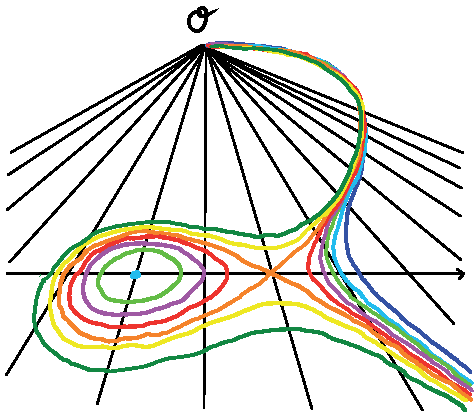
\includegraphics[scale=1]{img/bem_11_7.pdf}
		\caption{$y^2 = x^3 - 3x + s$ für \textcolor{Green4}{$s = 5$}, \ \textcolor{yellow}{$s=3$}, \ \textcolor{Orange2}{$s=2$}, \ \textcolor{red}{$s=1$}, \ \textcolor{Magenta1}{$s=0$}, \ \textcolor{green}{$s=-1$}, \ \textcolor{cyan}{$s=-1.999$}, \ \textcolor{RoyalBlue3}{$s=-5$}}
	\end{figure}
	Das Bild ist perspektivisch so verzerrt, dass der unendlich ferne Punkt $\oh$, der für die Richtung der $y$-Achse steht, am Horizont erscheint.
\end{bem}

\begin{satz}[Vereinfachte Weierstraßgleichungen]
\label{satz_11.8}
	Sei $E_F(k)$ eine elliptische Kurve mit $F$ in der langen Weierstraßform \eqref{eq_lang-weier}. \begin{enumerate}[(i)]
		\item Falls $\Char(k) \neq 2$, ist die Abbildung
		\begin{equation}
		\begin{aligned}
			\Phi \colon \PP^2(k) &\longrightarrow 2\PP^2(k) \\
			[r:s:t] &\longmapsto \benbrace*{r : s + \frac{a_1}{2}r + \frac{a_3}{2}t : t}
		\end{aligned}
		\end{equation}
		bijektiv und es ist $\Phi(E_f(k)) = E_{H_1}(k)$ ebenfalls eine elliptische Kurve mit $H_1(X,Y,Z) = Y^2Z - X^3 - \frac{1}{4}b_2 X^2Z - \frac{1}{2} b_4 XZ^2 - \frac{1}{4} b_6 Z^3$, wobei $b_2 = a_1^2 + 4a_2, b_4 = 2a_4 + a_1 a_3, b_6 = a_3^2 + 4a_6$.
		\item Falls $\Char(k) \neq 2$ und $\Char(k) \neq 3$, ist die Abbildung
		\begin{equation}
		\begin{aligned}
			\Psi\colon \PP^2(k) &\longrightarrow \PP^2(k) \\
			[r:s:t] &\longmapsto [36r + 3b_2 t : 216s : t]
		\end{aligned}
		\end{equation}
		bijektiv und es ist $\Psi(E_{H_1}(k)) = E_{H_2}(k)$ ebenfalls eine elliptische Kurve mit $H_2(X,Y,Z) = Y^2Z - X^3 + 27c_4 XZ^2 + 54 c_6 Z^3$, wobei $c_4 = b_2^2 - 24b_4, c_6 = -b_2^3 + 36b_2b_4 - 216b_6$.
	\end{enumerate}
\end{satz}

\begin{bem}
	Wir können die lange Weierstraßgleichung im Fall $\Char(k) \neq 2$ also stets zur affinen Gleichung $y_2 = x^3 + a_2x^2 + a_4 x + a_6$ vereinfachen; falls $\Char(k) \neq 2$ und $\Char(k)= \neq 3$ gilt, sogar zu $y^2 = x^3 + a_4 x + a_6$. Wir nennen diese Gleichung die \Index{kurze Weierstraßform}, das entsprechende Polynom dann das \bet{kurze Weierstraßpolynom}.
\end{bem}

\begin{bem}
	Auch im Fall $\Char(k) = 2$ lässt sich die lange Weierstraßgleichung vereinfachen, das ist nicht schwierig, wenn $a_1 \neq 0$, aber auch für $a_1 = 0$ möglich. Wir behandeln dies hier nicht näher.
\end{bem}

\begin{bew}
	Zunächst zu (i): \begin{itemize}
		\item $\Phi$ ergibt als Abbildung nur Sinn, wenn $2$ invertierbar ist in $k$, das heißt, falls $\Char(k) \neq 2$ ist. $\Phi$ ist dann bijektiv, da $\Phi$ die Umkehrabbildung $\Phi^{-1}([r:s:t]) = \benbrace*{r : s - \frac{a_1}{2}r - \frac{a_3}{2}t : t}$ hat.
		\item Weiter bezeichnen wir mit $\Phi, \Phi^{-1}$ auch die zugehörigen (affinen) Abbildungen $\Phi, \Phi^{-1}\colon k^3 \longrightarrow k$,\linebreak $\Phi(r,s,t) = \enbrace*{r,s+ \frac{a_1}{2}r + \frac{a_3}{2}t, t}$ bzw. $\Phi^{-1}(r,s,t) = \enbrace*{r,s - \frac{a_1}{2}r - \frac{a_3}{2}t,t}$. Nun können wir mit den im Satz angegebenen Zahlen $b_2,b_4,b_6$ nachrechnen, dass $H_1(X,Y,Z) = F\enbrace*{X,Y - \frac{a_1}{2}X - \frac{a_3}{2}Z,Z}$:
		\begin{equation}
		\begin{aligned}
			& \quad \ F\enbrace*{X,Y-\frac{a_1}{2}X-\frac{a_3}{2}Z,Z} \\
			&= \enbrace*{Y- \frac{a_1}{2} X - \frac{a_3}{2}Z}^2 Z + a_1 X \enbrace*{Y - \frac{a_1}{2} X - \frac{a_3}{2}Z}Z + a_3 \enbrace*{Y - \frac{a_1}{2} X - \frac{a_3}{2} Z}Z^2 \\
			& \quad \ - X^3 - a_2X^2Z - a_4 XZ^2 - a_6Z^3 \\
			&= Z \cdot \enbrace*{Y^2 - 2Y \enbrace*{\frac{a_1}{2}X + \frac{a_3}{2} Z} + \enbrace*{\frac{a_1^2}{4} X^2 + 2 \cdot \frac{a_1 a_3}{4} XZ + \frac{a_3^2}{4} Z^2}} \\
			& \quad \ + a_1XYZ - \frac{a_1^2}{2} X^2 Z - \frac{a_1 a_3}{2} XZ^2 + a_3 YZ^2 - \frac{a_1 a_3}{2} XZ^2 - \frac{a_3^2}{2} Z^3 - X^3 - a_2 X^2 Z - a_4 XZ^2 - a_6Z^3 \\
			&= Y^2 Z - X^3 + \enbrace*{-\frac{a_1^2}{4} - a_2} X^2 Z + \enbrace*{- \frac{a_1 a_3}{2} - a_4} XZ^2 + \enbrace*{- \frac{a_3^2}{4} - a_6} Z^3 \\
			&= Y^2 Z - X^3 - \frac{1}{4} b_2 X^2 Z - \frac{1}{2} b_4 XZ^2 - \frac{1}{4} b_6 Z^3 = H_1(X,Y,Z)
		\end{aligned}
		\end{equation}
		\item Es folgt $H_1(r,s,t) = F(\Phi^{-1}(r,s,t))$, also gilt $F(r,s,t) = 0$ genau dann, wenn $H_1(\Phi(r,s,t))=0$, sodass $\Phi (E_F(k)) = \cc_{H_1}(k)$ folgt. Es bleibt zu zeigen, dass $\cc_{H_1}(k)$ nicht-singulär ist: Mit der Kettenregel rechnen wir nach:
		\begin{equation}
		\begin{aligned}
			\frac{\der H_1}{\der X}(r,s,t) &= \frac{\der F}{\der X}(\Phi^{-1}(r,s,t)) - \frac{a_1}{2} \frac{\der F}{\der Y}(\Phi^{-1}(r,s,t)) \\
			\frac{\der H_1}{\der Y}(r,s,t) &= \frac{\der F}{\der Y} (\Phi^{-1}(r,s,t)) \\
			\frac{\der H_1}{\der Z}(r,s,t) &= -\frac{a_3}{2} \frac{\der F}{\der Y} \Phi^{-1}(r,s,t) + \frac{\der F}{\der Z}(\Phi^{-1}(r,s,t))
		\end{aligned}
		\end{equation}
		\item Ist $P = [r:s:t] \in \cc_{H_1}(\overline{k})$, dann ist $\Phi^{-1}(P) = \Phi^{-1}([r:s:t])$ als Punkt der Kurve $\cc_F(\overline{k})$ nicht-singulär, da $F$ elliptische Kurve ist. Die drei Ableitungen von $F$ in $\Phi^{-1}(P)$ sind also nicht alle $= 0$, also sind auch die drei Ableitungen von $H_1$ in $(r,s,t)$ nicht alle $=0$. Also ist $P$ auf $\cc_{H_1}(\overline{k})$ nicht-singulär.
	\end{itemize}
	Zu (ii): $\Psi$ hat die Inverse $[r:s:t] \mapsto \benbrace*{\frac{1}{36} r - \frac{b_2}{12}t : \frac{1}{216} s : t}$, da wegen $\Char(k) \neq 2, \neq 3$ die Zahlen $\frac{1}{36}, \frac{1}{12}, \frac{1}{216} = \frac{1}{2^3 \cdot 3^3}$ in $k$ existieren, und leicht zu bestätigen ist, dass $\Psi(\Psi^{-1}([r:s:t])) = [r:s:t]$ gilt. Durch geduldiges Nachrechnen zeigt man $H_2(X,Y,Z) = 2^6 3^6 \cdot H_1 \enbrace*{\frac{1}{36} X - \frac{b_2}{12}Z, \frac{1}{216} Y,Z}$, daraus folgt $H_1(r,s,t) = 0$ genau dann, wenn $H_2(\Psi(r,s,t))=0$, das heißt $\Psi(E_{H_1}(k)) = \cc_{H_2}(k)$. Wieder mit der Kettenregel kann auch die Nicht-Singularität von $\cc_{H_2}$ gezeigt werden. \qed
\end{bew}

Wir definieren zwei wichtige Kennzahlen projektiver Kurven wie folgt:
\begin{defn}[Diskriminante, $j$-Invariante]
	Sei $\cc_F(k)$ die projektive ebene Kurve zum langen Weierstraßpolynom \eqref{eq_lang-weier}. Dann heißt die Zahl
	\[ \Delta = \Delta(\cc_F(k)) = -b_2^2 b_8 - 8b_4^3 - 27b_6^2 + 9b_2b_4b_6 \]
	mit $b_2 = a_1^2 + 4a_2, b_4 = 2a_4 + a_1 a_3, b_6 = a_3^2 + 4a_6$ und $b_8 = a_1^2 a_6 + 4a_2 a_6 - a_1a_3a_4 + a_2 a_6^2 - a_4^2$ die \Index{Diskriminante} der Kurve $\cc_F(k)$. Die Zahl 
	\[ j = j(\cc_F(k)) := \frac{(b_2^2 - 24b_4)^3}{\Delta} = \frac{c_4^3}{\Delta} \]
	heißt die \bet{$j$-Invariante} der Kurve $\cc_F(k)$. \index{j-Invariante@$j$-Invariante}
\end{defn}

\begin{bem}
	\begin{itemize}
		\item Die $j$-Invariante legt die Isomorphieklasse der elliptischen Kurve über $\overline{k}$ fest: Zwei elliptische Kurven sind isomorph über $\overline{k}$ genau dann, wenn sie dieselbe $j$-Invariante besitzen (ohne Beweis).
		\item $j$ ist unabhängig von der Wahl der speziellen Kurvengleichung.
	\end{itemize}
\end{bem}

\begin{bem}
	Die Diskriminante einer Kurve $\cc_F(k)$ ist ein nützliches Hilfsmittel, um zu testen, ob eine Kurve, die durch eine lange Weierstraßgleichung gegeben ist, nicht-singulär (und damit elliptisch) ist:
\end{bem}

\begin{satz}
	Sei die Kurve $\cc_F(k)$ gegeben durch das lange Weierstraßpolynom $F$. Dann ist $\cc_F(k)$ nicht-singulär genau dann, wenn $\Delta(\cc_F(k)) \neq 0$ ist.
\end{satz}

Mit der angegebenen Formel für $\Delta$ ist dies auch rechnerisch leicht zu testen -- wichtig, um elliptische Kurven für die Anwendungen zu konstruieren. Dieses Diskriminantenkriterium zeigen wir im nächsten Abschnitt.
\nextlecture
\subsubsection{Das Diskriminantenkriterium}
\begin{defn}[Diskriminante]
	Sei $\cc_F(k)$ die projektive ebene Kurve zum langen Weierstraßpolynom \marginnote{[12]}
	\[ F(X,Y,Z) = Y^2Z + a_1XYZ + a_3YZ^2 - X^3 - a_2X^2Z - a_4 XZ^2 - a_6Z^3. \]
	Dann heißt die Zahl
	\[ \Delta = \Delta(\cc_F(k)) = -b_2^2 b_8 - 8b_4^3 - 27b_6^2 + 9b_2b_4b_6 \]
	mit $b_2 = a_1^2 + 4a_2, b_4 = 2a_4+a_1a_3, b_6 = a_3^2+4a_6$ und $b_8 = a_1^2 a_6 + 4a_2a_6-a_1a_3a_4 + a_2a_3^2 - a_4^2$ die \Index{Diskriminante} der Kurve $\cc_F(k)$.
\end{defn}

\begin{bem}
	Im Fall einer Kurve $\cc_F(k)$ in einer kurzen Weierstraßform $f(x,y) = y^2-x^3-ax-b$ haben wir $\Delta(\cc_F(k)) = -8 \cdot (2a)^3 - 27 \cdot (4b)^2 = -16 \cdot (4a^3 + 27b^2)$, da $a_1 = 0, a_3 = 0, a_2 = 0, a_4 = a, a_6 = b$, also $b_2 = 0, b_4 = 2a, b_6 = 4b, b_8 = -a^2$. (vgl. Übungsaufgabe 3 auf Blatt 4).
\end{bem}

Wir zeigen das Diskriminantenkriterium:
\begin{satz}[Diskriminantenkriterium]
\label{satz_12.3}
	Sei die Kurve $\cc_F(k)$ gegeben durch das lange Weierstraßpolynom $F$. Dann ist $\cc_F(k)$ nicht-singulär genau dann, wenn $\Delta(\cc_F(k)) \neq 0$ ist.
\end{satz}

\begin{bem}
	\begin{itemize}
		\item Bei diesem Kriterium, wenn $\Delta \neq 0$, erhalten wir, dass $\cc_F(\overline{k})$ über dem algebraischen Abschluss $\overline{k}$ keine singulären Punkte enthält (insbesondere auch über $k$, aber über $\overline{k}$ ist eben noch stärker). Deswegen haben wir uns bei unserer Definition von "nicht-singuläre Kurve" auf $\overline{k}$ bezogen, was wegen Satz~\ref{satz_12.3} also mathematisch leichter wird. Für $\Char(k) \neq 2$ kann es aber nicht sein, dass $\cc_F$ über $k$ keine singulären Punkte hat und über $\overline{k}$ hingegen schon.
		\item Das Kriterium ist in der Praxis nützlich, da eine Kurve in Weierstraßform (die vielleicht per Zufallsgenerator für die Koeffizienten erzeugt worden ist), damit leicht auf Nicht-Singularität durch Berechnung der einfachen Formel für $\Delta$ getestet/überprüft werden kann.
		\item Der Beweis unterscheidet wesentlich die Fälle $\Char(k) = 2, \Char(k) = 3$ und sonst.
	\end{itemize}
\end{bem}

\begin{bew}
	Die Kurve $\cc_F(k)$ ist nicht-singulär genau dann, wenn ihre affine Kurve $\cc_F(k)$ mit $f(x,y) = y^2 + a_1xy + a_3y - x^3 - a_2x^2 - a_4 x - a_6$ nicht-singulär ist. Wir zeigen den Satz deswegen im Affinen (der einzige nicht-affine Punkt $\oh = [0:1:0]$ der Kurve ist immer regulär, vgl. Bemerkung~\ref{bem_11.5}). Nun enthält $\cc_F(\overline{k})$ einen singulären Punkt $(r,s)$ genau dann, wenn
	\[ f(r,s) = 0 \qquad \underbrace{\frac{\der f}{\der x} (r,s)}_{a_1 s - 3r^2 - 2a_2r - a_4} = 0 \qquad \underbrace{\frac{\der f}{\der y} (r,s)}_{=2s + a_1 r + a_3} = 0 \]
	gilt. Wir unterscheiden weiter mehrere Fälle nach dem Wert der Charakteristik von $k$.
\end{bew}

\begin{bew}[1. Fall: $\Char(k)= 2$ und $a_1 = 0$]
	\begin{description}
		\item["$\Leftarrow$":] Dann ist hier $b_2 = b_4 = 0, b_6 = a_3^2, \Delta = -27a_3^4 = a_3^4$. Weiter gilt $\frac{\der f}{\der y} = a_3$, sodass, falls ein singulärer Punkt existiert, dann $a_3 = 0$ und $\Delta = 0$ folgt.
		\item["$\Rightarrow$":] Ist $\Delta = 0$, folgt $\frac{\der f}{\der y} = 0$. Nun existieren $r,s \in \overline{k}$ mit $r^2 + a_4=0, s^2 + a_3s = r^3 + a_2r^2 + a_4r + a_6$, also ist $(r,s) \in \aff^2(\overline{k})$ singulärer Punkt auf $\cc_f(\overline{k})$.
	\end{description}
\end{bew}

\begin{bew}[2. Fall: $\Char(k) = 2$ und $a_1 \neq 0$]
	In Charakteristik $2$ gilt:
	\begin{equation}
	\begin{aligned}
		\Delta &= -a_4^4 (a_1^2 a_6 - a_1 a_3 a_4 + a_2 a_3^2 - a_4^2) - 27a_3^4 + a_1^3 a_3^3 \\
		&= a_1^6 a_6 + a_1^5 a_3a_4 + a_1^4a_2a_3^2 + a_1^4a_4^2 + a_1^3 a_3^3 +a_3^4.
	\end{aligned}
	\end{equation}
	\begin{description}
		\item["$\Leftarrow$":] Hat $\cc_f(\overline{k})$ einen singulären Punkt $(r,s)$, so ist $f(r,s) = 0$, das heißt $a_1 s + r^2 + a_4 = 0$ und $a_1 r + a_3 = 0$. Da $a_1 \neq 0$, folgt $r = \frac{a_3}{a_1}$ und $s = \frac{a_3^2+a_1^2a_4}{a_1^3}$. Durch einsetzen in $f(r,s)$ folgt $0 = f(r,s) = \Delta a_1^{-6}$, also $\Delta = 0$.		
		\item["$\Rightarrow$":] Ist $\Delta = 0$, definieren wir $r,s$ wie oben, dann ist $f(r,s) = \Delta a_1^{-6}$, also $f(r,s) = 0$, womit ein singulärer Punkt konstruiert ist.
	\end{description}
\end{bew}

\begin{bew}[3. Fall: $\Char(k)=3$]
	Via Rechnen in Charakteristik $3$ folgt $\Delta = -b_2^2 b_8 - 8b_4^3$. Betrachte die Abbildung $\Phi\colon \cc_F(k) \rightarrow \cc_{H_1}(k)$ aus Satz~\ref{satz_11.8}(i), die die lange Weierstraßform $F$ auf die kurze Form $H_1$ bringt. Es ist $\Delta(\cc_{H_1}(k)) = \Delta(\cc_F(k))$ durch Nachrechnen, somit genügt es ohne Einschränkung, das Diskriminantenkriterium für die kurze Form $H_1$ zu zeigen.
\end{bew}

\begin{bew}[Fortsetzung 3. Fall]
	Die Kurve $\cc_{H_1}(\overline{k})$ enthält genau dann einen singulären Punkt, wenn es $r,s \in \overline{k}$ gibt mit
	\[ s^2 - r^3 - \frac{1}{4} b_2 r^2 - \frac{1}{2}b_4 r - \frac{1}{4} b_6 = 0, \qquad 3r^2 + \frac{1}{2} b_2r + \frac{1}{2} b_4 = 0,  \qquad 2s = 0, \]
	das heißt falls $r$ eine doppelte Nullstelle des Polynoms $\sigma(x) := x^3 + \frac{1}{4} b_2 x^2 + \frac{1}{2} b_4x \frac{1}{4} b_6$ ist, sprich $\sigma(r) = 0 = \sigma'(r)$ ist. \\
	Über $\overline{k}$ zerfällt $\sigma$ in drei Linearfaktoren $\sigma(x) = (x-\alpha_1)(x-\alpha_2)(x-\alpha_3)$ mit $\alpha_i \in \overline{k}$. Nun hat ein Polynom $\sigma$ genau dann eine doppelte Nullstelle, falls seine Diskriminante $\disc(\sigma) := (\alpha_1 - \alpha_2)^2 (\alpha_1 - \alpha_3)^2 (\alpha_2 - \alpha_3)^2$ verschwindet, vgl. Bemerkung~\ref{bem_12.14}.
\end{bew}

\begin{bew}[Fortsetzung]
	Somit ist im dritten Fall zu zeigen: $\Delta = 0 \Leftrightarrow \disc(\sigma)=0$. \\
	Wegen $\disc(x^3 + ux^2 + vx + w) = u^2v^2 - 4u^3w - 4v^3 - 27w^2 + 18uvw$, vgl. Korollar~\ref{kor_12.16}, erhalten wir mit $u = \frac{b_2}{4}, v = \frac{b_4}{2}, w= \frac{b_6}{4}$ dann in Charakteristik $3$, dass $\disc(\sigma) = \frac{1}{64} b_2^2 b_4^2 - \frac{1}{64} b_2^3 b_6 - \frac{1}{2} b_4^3$. Wegen $4 b_8 = b_2 b_6 - b_4^2$ erhalten wir $\disc(\sigma) = \frac{1}{16} (-b_2^2b_8 - 8b_4^3) = \frac{1}{16} \Delta$. Aus dieser Formel folgt die Behauptung im dritten Fall.
\end{bew}

\begin{bew}[4. Fall: $\Char(k) > 3$ oder $\Char(k) = 0$]
	Mit der Bijektion $\Psi \circ \Phi \colon \cc_F(k) \rightarrow \cc_{H_2}(k)$ zum kurzen Weierstraßpolynom $H_2$ (Satz~\ref{satz_11.8}(ii)) bzw. $h_2(x,y) = y^2 - x^3 + 27c_4x + 54c_6$ mit $c_4 = b_2^2 - 24b_4, c_6 = -b_2^3 + 36b_2 b_4 - 216 b_6$, folgt durch Untersuchung der Ableitungen wieder $\cc_F(k)$ nicht-singulär genau dann, wenn $\cc_{H_2}(k)$ nicht-singulär. Wir berechnen $\Delta(\cc_{H_2}(k)) = 2^6 3^9 \cdot (c_4^3-c_6^2) = \dots = 2^{12} 3^{12} \Delta(\cc_F(k))$, also genügt es, die Behauptung für $\cc_{H_2}(k)$ zu zeigen. Wie im dritten Fall haben wir:
	\[ \cc_{H_2}(\overline{k}) \text{ enthält singulären Punkt } \quad \Leftrightarrow \quad \sigma(x) = x^3 \underbrace{- 27c_4}_{v} x \underbrace{- 54 c_6}_{w} \text{ hat doppelte Nullstelle } \quad \Leftrightarrow \quad \disc(\sigma)=0 \]
	Wegen der Formel in Korollar~\ref{kor_12.16} für $\disc(\sigma)$ folgt mit $u = 0, v = -27c_4, w= - 54c_6$:
	\[ \disc(\sigma) = 0 \quad \Leftrightarrow \quad 4 \cdot 27^3 c_4^3 - 27 \cdot 54^2 c_6^2 = 0 \quad \Leftrightarrow \quad c_4^3 - c_6^2 = 0. \]
	Daraus folgt die Behauptung. \qed
\end{bew}

Theoretische Ergänzungen zu unserer Definition von $\Delta(\cc_F(k))$:
\begin{defn}[Diskriminante eines Polynoms]
	Die \bet{Diskriminante eines Polynoms} $\sigma \in k[x], n := \deg(\sigma) \geq 1$, ist \index{Diskriminante!eines Polynoms}
	\[ \disc(\sigma) := \prod_{1 \leq i < j \leq n} (\alpha_i - \alpha_j)^2 = (-1)^{\frac{n(n-1)}{2}} \prod_{i \neq j} (\alpha_i - \alpha_j) \in \overline{k},\]
	falls $\alpha_1, \dots, \alpha_n \in \overline{k}$ die Nullstellen von $\sigma \in \overline{k}$ bezeichnen.
\end{defn}

\begin{bem}
	Man vergleiche dies mit der Diskriminante $\disc(\sigma) = p^2-4q$ eines quadratischen Polynoms $\sigma(x) = x^2+px+q \in k[x]$, wir haben $\alpha_{1,2} = -\frac{p}{2} \pm \sqrt{\frac{p^2}{4} - q} = -\frac{p}{2} \pm \frac{1}{2} \sqrt{p^2 -4q}$, also genau $(\alpha_1 - \alpha_2)^2 = \disc(\sigma)$. Ist dies $=0$, ist $\alpha_1 = \alpha_2$ eine doppelte Nullstelle von $\sigma$.
\end{bem}

\begin{bem}
\label{bem_12.14}
	$\disc(\sigma)$ verschwindet genau dann, wenn $\sigma$ über $\overline{k}$ eine doppelte Nullstelle hat. Dies folgt unmittelbar aus der Definition von $\sigma$.
\end{bem}

\begin{bem}
\label{bem_12.15}
	\begin{itemize}
		\item Ist $\sigma \in k[x], n = \deg(\sigma) \geq 1$, ein normiertes Polynom, kann die Beziehung $\disc(\sigma) = (-1)^{n(n-1)/2} \cdot \Res(\sigma, \sigma')$ mit der in Definition~\ref{def_10.5} behandelten Resultante gezeigt werden.
		\item Aus dieser wichtigen Formel folgt wegen unserer Definition für die Resultante, dass stets $\disc(\sigma) = k$ gilt.
	\end{itemize}
\end{bem}

\begin{kor}
\label{kor_12.16}
	Es gilt $\disc(x^3+ux^2+vx+w) = u^2v^2 - 4wu^3 - 4v^3 - 27w^2 + 18uvw$. 
\end{kor}

\minisec{Beweis}
	Für $\sigma(x) = x^3 + ux^2 + vx + w$ und $\sigma'(x) = 3x^2+2ux+v$ ist nach Defintion~\ref{def_10.5}: \marginnote{Genaue Rechnung im Skript!}
	\[ M(\sigma,\sigma') = \begin{pmatrix}
	w & 0 & v & 0 & 0 \\ 
	v & w & 2u & v & 0 \\ 
	u & v & 3 & 2u & v \\ 
	1 & u & 0 & 3 & 2u \\ 
	0 & 1 & 0 & 0 & 3
	\end{pmatrix} \]
	Durch Berechnung von $\Res(\sigma) = \det(M(\sigma,\sigma'))$ und $(-1)^{3 \cdot (3-1)/2} = -1$ folgt die Behauptung. \qed
	
\nextlecture
\subsubsection{Die Gruppenstruktur elliptischer Kurven}
	Sei $E(k)$ eine elliptische Kurve über einem Körper $k$. \marginnote{[13]}
	
\begin{satz}
\label{satz_13.1}
	\begin{enumerate}[(a)]
		\item Seien $P,Q \in E(k), P \neq Q$, und $G=G(P,Q) \subseteq \PP^2(k)$ die projektive Gerade, die $P$ und $Q$ verbindet. Dann hat $G$ noch einen dritten Schnittpunkt mit $E(k)$ gemäß Vielfachheiten gezählt (das heißt, eventuell $P$ bzw. $Q$ selbst, falls $m(P;G,E(k)) = 2$ bzw. $m(Q;G,E(k)) = 2$).
		\item Sei $G$ die Tangente an $E(k)$ im Punkt $P \in E(k)$. Dann hat $G$ noch einen dritten Schnittpunkt mit $E(k)$ gemäß der Vielfachheiten gezählt (das heißt, eventuell $P$ selbst, falls $m(P;G,E(k)) = 3$).
	\end{enumerate}
\end{satz}

\begin{bew}
	Als Ergänzung zum Satz von Bézout haben wir Satz~\ref{satz_10.15} kennen gelernt, der im Spezialfall $\deg(F_1) = 1,\linebreak \deg(F_2) = 3$ dann $\sum_{P \in \cc_{F_1} \cap \cc_{F_2}} m(P;\cc_{F_1},\cc_{F_2}) \in \{0,1,3\}$ liefert (siehe Beispiel~\ref{bsp_10.16}). Also gilt auch hier: \linebreak $\sum_{R \in G \cap E(k)} m(R;G,E(k)) \in \{0,1,3\}$.
	\begin{description}
		\item[zu (a):] Ist $G = G(P,Q)$, folgt $2 \leq  \#(G \cap E(k)) \leq \sum_{R \in G \cap E(k)} m(R;G,E(k)) \in \{0,1,3\}$. Das geht nur, wenn die Vielfachensumme $3$ ist, also existiert ein $R \in G \cap E(k)$ \begin{itemize}
			\item mit $R \notin \{P,Q\}$, falls $m(P;G,E(k)) = 1 = m(Q;G,E(k))$,
			\item oder mit $R = P$, falls $m(P;G,E(k)) = 2$
			\item oder mit $R = Q$, falls $m(Q;G,E(k)) = 2$.
		\end{itemize} 
		\item[zu (b):] Ist $G$ die Tangente an $E(k)$ in $P \in E(k)$, ist $m(P;G,E(k)) \geq 2$ nach Satz~\ref{satz_9.22}. Es folgt wie im Beweis zu (a) wieder, dass die Vielfachensumme $3$ ist, also die Existenz eines $R \in G \cap E(k)$ mit $R \neq P$, falls $m(P;G,E(k)) = 2$ und $R = P$, falls $m(P;G,E(k)) = 3$ gilt. \qed
	\end{description}
\end{bew}

\begin{bsp}
	Betrachte die elliptische Kurve $E(k)$ zur (kurzen) Weierstraßgleichung $y^2 = x^3 - 3x + 3$. Jede Gerade, die $E(k)$ in zwei Punkten schneidet, schneidet $E(k)$ in einem dritten Punkt, gemäß Vielfachheit gezählt. Der dritte Schnittpunkt kann auch $\oh \in g_\infty$ sein. \todo{Bild texen!}
	\newpage
	\begin{figure}[h]
		\centering
		\begin{tikzpicture}[scale=1]
			\draw [thick,samples=500,smooth,domain=-2.10378:2.4,variable=\x,blue] plot ({\x},{(\x*\x*\x-3*\x+3)^(0.5)});
			\draw [thick,smooth,domain=-2.10378:2.4,variable=\x,blue] plot ({\x},{-(\x*\x*\x-3*\x+3)^(0.5)});
			
			\draw (-2.1038,0) node[fill,circle,inner sep=2pt,red]{};
			\draw (-2.2,0) node[align=right,anchor=east]{$S$};
			\draw [very thick](-2.1038,-2.5) -- (-2.1038,2.5);
			
			\draw (.292037,-1.46588) node[fill,circle,inner sep=2pt,red]{};
			\draw (.292037,-1.46588) node[align=left,anchor=north west]{$W$};
			\draw [very thick,smooth,domain=-.7:1.3,variable=\x] plot ({\x},{.936007*\x-1.73923});
			
			\draw (1.8,-1.85257) node[fill,circle,inner sep=2pt,red]{};
			\draw (1.8,-1.85257) node[align=left,anchor=south west]{$U$};
			\draw (-.31049,1.97523) node[fill,circle,inner sep=2pt,red]{};
			\draw (-.31049,1.97523) node[align=left,anchor=south west]{$U*U$};
			\draw [very thick,smooth,domain=-.7:2.2,variable=\x] plot ({\x},{-1.8137*\x+1.4121});
			
			\draw (-1.8,-1.6025) node[fill,circle,inner sep=2pt,red]{};
			\draw (-1.8,-1.6025) node[align=left,anchor=north,yshift=-.2cm]{$P$};
			\draw (.8,1.05451) node[fill,circle,inner sep=2pt,red]{};
			\draw (.8,1.05451) node[align=left,anchor=north west]{$Q$};
			\draw (2.044337,2.32614) node[fill,circle,inner sep=2pt,red]{};
			\draw (2.044337,2.32614) node[align=left,anchor=north west]{$P*Q$};	
			\draw [very thick,smooth,domain=-2.5:2.5,variable=\x] plot ({\x},{1.02193*\x+0.236968});
		\end{tikzpicture}
		\caption{Veranschaulichung der Definition~\ref{def_13.4} an dem Beispiel $y^2=x^3-3x+3$: Für zwei verschiedene Punkte $P,Q$ definieren wir $P*Q$ als den dritten Schnittpunkt der Gerade durch $P$ und $Q$. Das kann wieder $P$ oder $Q$ sein, falls die Gerade eine Tangente durch $P$ oder $Q$ ist. Für einen Punkt $U$ setzen wir $U * U$ als den weiteren Schnittpunkt der Tangente durch $U$; dieser kann auch $\oh$ sein (z.B. im Fall von $S$). Ein Wendepunkt $W$ ist bereits dreifacher Schnittpunkt, daher definieren wir hier $W * W = W$.}
	\end{figure}
\end{bsp}

Wir möchten auf $E(k)$ eine Verknüpfung "$+$" erklären, also eine Punkteaddition $P + Q$, bei der wiederum ein Punkt auf der elliptischen Kurve herauskommt. Den dritten Schnittpunkt, den die Gerade $G(P,Q)$ durch zwei Punkte $P$ und $Q$ auf $E(k)$ mit $E(k)$ hat laut Satz~\ref{satz_13.1}, bezeichnen wir mit $P * Q$.

\begin{defn}[dritter Schnittpunkt]
\label{def_13.4}
	Für $P,Q \in E(k)$, $P \neq Q$ definieren wir also:
	\[ P * Q := \begin{cases}
		R \in (G(P,Q) \cap E(k)) \setminus \{P,Q\}, & \text{falls } m(P;G,E(k)) = 1 = m(Q;G,E(k)) \\
		P, & \text{falls } m(P;G,E(k)) = 2 \\
		Q, & \text{falls } m(Q;G,E(k)) = 2,
	\end{cases} \]
	sowie
	\[ P * P := \begin{cases}
		R \in (T_P(E(k)) \cap E(k)) \setminus \{P\}, & \text{falls } m(P;T_p(E(k)),E(k)) = 2 \\
		P, & \text{falls } m(P;T_P(E(k)),E(k)) = 3 \text{ (d.h. falls } P \text{ Wendepunkt)}
	\end{cases} \]
\end{defn}

\begin{bem}
	\begin{itemize}
		\item Der unendlich ferne Punkt $\oh \in E(k)$ erfüllt $\oh * \oh = \oh$, da er ein Wendepunkt ist.
		\item Weiter ist offensichtlich $P * Q = Q * P$ aufgrund der Definition.
		\item Es gilt: $R = P * Q \Rightarrow P = Q * R \Rightarrow Q = R * P$, das heißt $P * (P * Q) = Q$ für alle $P,Q \in E(k)$. \hfill [\#]
		\item Damit gilt auch $P * Q = P * R \Leftrightarrow Q = R$, denn $P * Q = P * R \Rightarrow P*(P*Q)=P*(P*R) \Rightarrow Q=R$.
	\end{itemize}
\end{bem}

\begin{bem}
	Man beachte, dass für $P = [a:b:1] \in \PP^2(k) \cap \iota(\aff^2(k))$ die Gerade $G(P,Q) = G(c,0,-a) = \{ [x:y:z] \in \PP^2(k) : x - az = 0\}$ im Affinen eine Parallele zur $y$-Achse darstellt (Gleichung $x = a$). Für eine elliptische Kurve, die durch eine kurze Weierstraßform gegeben und (für $\Char(k) \neq 2$) symmetrisch zur $x$-Achse ist, wird typischerweise $P * \oh \neq P$ sein. Wegen $(\oh * \oh) * P = \oh * P$ einerseits, da $\oh * \oh = \oh$, und $\oh * (\oh * P) = P$ andererseits wegen [\#], kann die Verknüpfung $*$ also nicht assoziativ sein. Stattdessen setzen wir unsere Verknüpfung "$+$" wie folgt:
\end{bem}

\begin{defn}[Punkteaddition auf elliptischen Kurven]
	Für $P,Q \in E(k)$ definieren wir
	\[P + Q := \oh *(P * Q). \]
	Ist $E(k)$ in kurzer Weierstraßform und (für $\Char(k) \neq 2$) symmetrisch zur $x$-Achse, erhält man $P+Q$, indem man den dritten Schnittpunkt $P*Q$ von $G(P,Q)$ mit $E(k)$ dann noch an der $x$-Achse spiegelt, das heißt das Negative des $y$-Wertes nimmt.
\end{defn}

\begin{bem}
\label{bem_13.8}
	\begin{itemize}
		\item Es gilt $\oh + P = \oh * (\oh * P) = P$ nach [\#], das heißt $\oh$ ist neutrales Element bezüglich $+$.
		\item Es gilt $-P = \oh * P$, da $P + (\oh * P) = \oh * (P * (\oh * P)) = (P * (\oh * P)) * \oh = (P * (P * \oh)) * \oh = \oh$ nach [\#].
	\end{itemize}
\end{bem}
Es ist nicht auf Anhieb zu sehen, dass hier mit "$+$" eine elliptische Kurve $E(k)$ zu einer Gruppe $(E(k),+)$ wird, sprich, ob das Assoziativgesetz gilt.

\begin{lemma}
\label{lemma_13.9}
	Liegen drei Punkte $P,Q,R \in E(k)$ einer elliptischen Kurve auf einer projektiven Gerade $G$, so gilt $(P+Q) + R = \oh$ und umgekehrt. Dabei müssen $P,Q,R$ nicht notwendig verschieden sein.
\end{lemma}

\minisec{Beweis}
	Da $R = P *Q$ nach Voraussetzung, folgt $-R = \oh * R = \oh * (P * Q) = P+Q$. Umgekehrt gilt das ebenso. \qed
	
\begin{satz}[Elliptische Kurve mit Punktaddition ist abelsche Gruppe, Poincaré, 1901]
	Sei $k$ ein beliebiger Körper und $E(k)$ eine elliptische Kurve. Die Verknüpfung $+ \colon (P,Q) \mapsto P +Q$ macht $E(k)$ zu einer abelschen Gruppe $(E(k),+)$ mit neutralem Element $\oh$, das heißt:
	\begin{enumerate}[(i)]
		\item $P+\oh = P$ für alle $P \in E(k)$.
		\item Für alle $P \in E(k)$ existiert ein $Q \in E(k)$ mit $P+Q = \oh$; setze $-P := Q$.
		\item $P + Q = Q + P$ für alle $P,Q \in E(k)$.
		\item $(P+Q) + R = P+(Q+R)$ für alle $P,Q,R \in E(k)$.
	\end{enumerate}
\end{satz}

\minisec{Beweis}
	\begin{enumerate}[(i)]
		\item Siehe Bemerkung~\ref{bem_13.8}.
		\item Für $P \in E(k)$ setze $Q := \oh * P$, siehe Bemerkung~\ref{bem_13.8}.
		\item Klar aufgrund der Definition von $P+Q$.
		\item Beweis folgt im nächsten Vorlesungsteil. \qed
	\end{enumerate}
	
\begin{bem}
	\begin{itemize}
		\item Anstelle von $\oh$ könnte man prinzipiell jeden Punkt $Q \in E(k)$ zum neutralen Element von $+$ machen, indem man $U \oplus V := U + V - Q$ setzt: Dann ist $U \oplus Q = U + Q - Q = U, U \oplus(-U+2Q) = U-U+2Q-Q = Q$ und $(U \oplus V) \oplus W = U + V + W - 2Q = U \oplus (V \oplus W)$. Die Eigenschaft von Lemma~\ref{lemma_13.9} gilt immer noch, wenn für $Q$ ein Wendepunkt genommen wird. Nun kann eine elliptische Kurve bis zu neun Wendepunkte haben, vergleiche Übungsaufgabe 4 (a) auf Blatt 5.
		\item Die Wahl von $\oh := [0:1:0]$ als Wendepunkt von $E(k)$, das heißt mit $\oh * \oh = \oh$, hat den Vorteil, dass die explizite Formel für $+$ rechnerisch einfacher wird, weil dann die Gleichung von $E(k)$ in einfacher (langer oder kurzer) Weierstraßform vorliegt. Diese Formel wird in Satz~\ref{satz_13.13} bzw. Satz~\ref{satz_13.14} angegeben.
		\item Invertieren, das heißt Berechnen von $-P = P * \oh$, ist dann bei kurzer Weierstraßform in $\Char(k) \neq 2$ und $\Char(k) \neq 3$ besonders leicht: Man spiegelt $P$ an der $x$-Achse und erhält $-P$, das heißt ist $P = [a:b:c]$, gilt $-P = [a:-b:c]$. Schnittpunkte von $E(k)$ mit der $x$-Achse sind dann selbstinvers, das heißt für $P = [a:0:c] \in E(k)$ gilt $-P = P$.
	\end{itemize}
\end{bem}

\begin{bsp}
	Betrachte $E(\RR)$ mit der Gleichung $y^2 = x^3 + 17$ bzw. $Y^2Z = X^3 + 17Z^3$. Dann liegen $P = [-1:4:1]$ und $Q = [-2:3:1]$ auf der Kurve. Ihre Verbindungsgerade ist $G(P,Q) = \{ [x:y:z] \in \PP^2(\RR) : x-y+5z = 0\}$. Um $P+Q$ zu berechnen, bestimmen wir den dritten Schnittpunkt $P*Q$ von $G(P,Q)$ und $E(\RR)$ wie folgt: Setze $y = x + 5$ ein und erhalte $(x+5)^2 = x^3 + 17 \Leftrightarrow x^3 - x^2 - 10x - 8 = 0$. Da $x = -1, x = -2$ Nullstelle der linken Seite sind, führt Polynomdivision durch $(x+1)(x+2)$ zu $x^3-x^2-10x-8 = (x+1)(x+2)(x-4)$. Der Punkt $P * Q$ hat also die $x$-Koordinate $4$; da er auf $G$ liegt, folgt $P*Q = [4:9:1]$. Es folgt $P + Q = [4:-9:1]$.
\end{bsp}

Ist $E(k)$ gegeben durch das lange Weierstraßpolynom
\[ F(X,Y,Z) = Y^2Z + a_1 XYZ + a_3 YZ^2 - X^3 - a_2X^2Z - a_4 XZ^2 - a_6 Z^3 \]
bzw. $f(x,y) = y^2 + a_1xy + a_3y - x^3 - a_2x^2 - a_4x - a_6$, so möchten wir die Addition "$+$" für die Krypto-Anwendungen in einer expliziten Formel beschreiben:

\begin{satz}[Punkteaddition bei langer Weierstraßform]
\label{satz_13.13}
	Sei $E(k)$ gegeben durch das lange Weierstraßpolynom $F$. Dann gilt: \begin{enumerate}[(a)]
		\item $P = (u,v) \in E(k) \cap \aff^2(k) \Rightarrow -P = (u,-v-a_1u-a_3)$
		\item Sei $P = (u,v), Q = (r,s) \in E(k) \cap \aff^2(k)$. \begin{itemize}
			\item Ist $u = r$ und $v + s + a_1 u + a_3 = 0$, gilt $P + Q = \oh$.
			\item Sonst ist \marginnote{Beweis wäre langweiliges Nachrechnen\dots}
			\[ P + Q = (\underbrace{\lambda^2 + a_1 \lambda - a_2 - u - r}_{=:x_3}, -(\lambda + a_1) x_3 - \mu - a_3), \] wobei
			\[ \lambda = \frac{s-v}{r-u}, \quad \mu = \frac{vr - su}{r-u}, \quad \text{ falls } r \neq u, \]
			und
			\[ \lambda = \frac{3u^2 + 2a_2 u +a_4 - a_1 v}{2v + a_1u + a_3}, \quad  \mu = \frac{-u^3 + a_4 u + 2a_6 - a_3v}{2v + a_1u + a_3}, \quad \text{ falls } r = u. \]
		\end{itemize}
	\end{enumerate}
\end{satz}

Wir geben den Beweis für die Formel bei kurzer Weierstraßform, wo er leicht zu machen ist:
\begin{satz}[Punkteaddition bei kurzer Weierstraßform]
\label{satz_13.14}
	Ist $E(k)$ gegeben durch $f(x,y) = y^2 - x^3 - ax - b$, so gilt:
	\begin{enumerate}[(a)]
		\item Für $P = (u,v) \in E(k)$ gilt $-P = (u,-v)$.
		\item Für $P = (u,v), Q = (r,s)$ mit $P \neq -Q$ ist
		\[ P + Q = (\underbrace{\lambda^2 - u - r}_{=:x}, \lambda(u-x) - v), \]
		wobei
		\[ \lambda = \begin{cases}
			\frac{s-v}{r-u}, & \text{falls } P \neq Q \\
			\frac{3u^2+a}{2v}, & \text{falls } P = Q.
		\end{cases} \]
	\end{enumerate}
\end{satz}

\minisec{Beweis}
	(a) ist klar. Zu (b): Sei $P \neq \pm Q$. Haben $g(P,Q) = \{ (u+t,v + \lambda t) : t \in \RR\}$ mit $\lambda := \frac{s-v}{r-u}$, sowie $f(u+t, v+ \lambda t) = (v + \lambda t)^2 - (u+t)^3 - a(u+t) - b$ mit den Nullstellen $t = 0, t = r-u$. Eine weitere Nullstelle ist $t = x-u$. Die Nullstellensumme $0 + r-u + x - u = r + x - 2u$ ergibt den Koeffizienten vor $t^2$ des Polynoms, nämlich $\lambda^2 - 3u$; es folgt $x = \lambda^2 - u - r$. Die $y$-Koordinate des Punkts auf $g(P,Q)$ ist dann $v + \lambda(x - u)$, für $P+Q$ dann das Negative. \\
	Ist $Q = P, P \neq -P$ (das heißt $v \neq 0$), nimmt man die Tangente an $E(k)$ im Punkt $P$, also
	\begin{equation}
	\begin{aligned}
		t_P(E(k)) &= \{(x,y) : (-3u^2 - a)x + 2vy + v^2 - 2au - 3b = 0\} \\
		&= \{ (u+t, v+ \lambda t) : t \in \RR\}
	\end{aligned}
	\end{equation}
	mit der Steigung $\lambda := \frac{3u^2 + a}{2v}$. Der Rest der Rechnung geht wie eben; es folgt $x = \lambda^2$ (da $u=r$) und der angegebene $y$-Wert für $P+P$. \qed
\chapter{Gruppenwirkungen auf kubischen Komplexen} % (fold)
\label{cha:3}

\subsection*{Motivation}
\begin{enumerate}[(i)]
	\item Spezieller Fall des Satzes von \textsc{Cartan-Hadamard}: \marginnote{15.01. \\ \ [16]}
	
	Sei $X$ ein vollständiger einfach-zusammenhängender lokaler $\CAT$-Raum.
	Dann ist $X$ $\CAT$. Also:
	
	\[
		\left. \begin{array}{l}
			\text{lokale Eigenschaft: lokal } \CAT \\
			\text{globale Eigenschaft: einfach zusammenhängend}
		\end{array} \right\} \quad \Rightarrow \quad \text{global } \CAT
	\]
	Frage: Wie kann man die lokale $\CAT$-Eigenschaft testen?
	
	Für eine spezielle Klasse von Räumen -- kubische Komplexe -- kann man diese lokale Eigenschaft in eine kombinatorische Eigenschaft übersetzen und somit leichter testen ($\Rightarrow$ \textsc{Gromov}'s Link Condition).
	\item Fragestellung: Wann besitzt die simpliziale Wirkung einer endlich erzeugten Gruppe $G$ auf einen $\CAT$ kubischen Komplex einen Fixpunkt?
	
	Für $\CAT$ kubische Komplexe werden wir eine Methode sehen, um diese Fragestellung anzugehen.
\end{enumerate}

\section{Kubische Komplexe}
\label{sec:3.1}
	Grobe Idee: Wir bauen einen topologischen Raum aus Würfeln.\\
	Als Konvention legen wir fest: $[0,1]^0 = \{0\}$.
	
\begin{definition}[Würfel, Seite]
\label{def:3.1}
	Sei $W:= [0,1]^n \subseteq (\RR^n,d_2)$ ein \Index{Würfel}.
	Eine \Index{Seite} $S \subseteq W$ ist gegeben durch
	\[
		S = S_1 \times \dots \times S_n \text{ mit } S_i \in \{ \{0\}, \{1\}, [0,1]\}.
	\]
	Die eingeschränkte euklidische Metrik auf $W$ bezeichnen wir mit $d_W$.
	Weiter definieren wir die \Index{Dimension} von $W$ wie folgt:
	\[
		\dim(W) := \dim(\sprod{W}) \text{ mit } \sprod{W} \text{ als } \RR-\text{Vektorraum}.
	\]
\end{definition}	
\newpage
\begin{beispiel}
\label{bsp:3.2}
	\mbox{} \\[-1.2cm]
	\begin{figure}[h]
		\centering
		\begin{tikzpicture}[scale=1.5,>=Latex]
			\draw [gray,thick,->] (-.1,0) -- (1.2,0);
			\draw [gray,thick,->] (0,-.1) -- (0,1.2);
			\draw [schraffiert=teal,thick] (0,0) -- (1,0) -- (1,1) -- (0,1) -- cycle;
			
			\draw [color=red,very thick] (0,1) -- (1,1);
			\draw [color=red] (1,0) node[fill,circle,inner sep=1.5pt]{};
			\draw [color=red] (1,1) node[right]{$[0,1] \times \{1\}$};
			\draw [color=red] (1,0) node[below]{$\{1\} \times \{0\}$};
		\end{tikzpicture}
		\caption{Zwei Seiten des Würfels $W = [0,1]^2$.}
	\end{figure}
\end{beispiel}

\begin{definition}[Verklebung, kubischer Komplex]
\label{def:3.3}
	Seien $W_1,W_2$ zwei Würfel und $S_1 \subseteq W_1$ und $S_2 \subseteq W_2$ Seiten.
	Eine Isometrie $\varphi \colon S_1 \rightarrow S_2$ heißt \Index{Verklebung} von $W_1$ und $W_2$.
	Sei nun $\mathcal{W}$ eine Familie von Würfeln und $\mathcal{V}$ eine Familie von Verklebungen von Würfeln aus $\mathcal{W}$ mit folgenden Eigenschaften:
	\begin{enumerate}[(i)]
		\item Kein Würfel ist mit sich selbst verklebt.
		\item Je zwei Würfel aus $\mathcal{W}$ sind höchstens einmal miteinander verklebt.
	\end{enumerate}
	Sei $\sim$ die durch
	\[
		x \sim y \quad :\Leftrightarrow \quad \text{es existiert ein } \varphi \in \mathcal{V} \text{ mit } x \in \dom(\varphi) \text{ und } \varphi(x) = y
	\]
	erzeugte Äquivalenzrelation auf $\bigcup_{W \in \mathcal{W}} W$. Die Menge
	\[
		X := \faktor{\enbrace*{ \bigcup_{W \in \mathcal{W}} W}}{\sim}
	\]
	heißt kubischer Komplex definiert durch $(\mathcal{W},\mathcal{V})$.
	Die Dimension von $X$ ist definiert durch
	\[
		\dim(X) := \sup\{ \dim(W) : W \in \mathcal{W}\}.
	\]
\end{definition}

\begin{beispiel}
\label{bsp:3.4}
	\mbox{} \\[-1.4cm]
	\begin{align*}
		\mathcal{W} := \ &\{W_1 = [0,1]^2, W_2 = [0,1]^2, W_3 = [0,1]\} \\
		\mathcal{V} := \ &\{\varphi_1 \colon \{0\} \times \{0\} \subseteq W_1 \rightarrow \{1\} \times \{1\} \subseteq W_2, \varphi_2 \colon [0,1] \times \{1\} \subseteq W_2 \rightarrow [0,1] = W_3\}
	\end{align*}
\end{beispiel}

\begin{figure}[h]
	\centering
	\begin{tikzpicture}[scale=1,>=Latex]
		\draw [thick,schraffiert=teal] (0,0) -- (1,0) -- (1,1) -- (0,1) -- cycle;
		\draw [thick,schraffiert=teal] (2,0) -- (3,0) -- (3,1) -- (2,1) -- cycle;
		\draw [very thick,color=red] (4,0) -- (5,0);
		\draw [very thick,color=red] (2,1) -- (3,1);
		
		\draw (.5,0) node[below]{$W_1$};
		\draw (2.5,0) node[below]{$W_2$};
		\draw (4.5,0) node[below]{$W_3$};
		
		\draw [color=Green4,->] (0,0) .. controls (-1,1) and (1,2.5) ..   (3,1);
		\draw [color=Green4,->] (2.5,1) to[out=90,in=90] (4.5,0);
		
		\draw [color=RoyalBlue2] (0,0) node[fill,circle,inner sep=2pt]{};
		\draw [color=RoyalBlue2] (3,1) node[fill,circle,inner sep=2pt]{};
		\draw [color=Green4] (4,1) node[right]{$\varphi_2$};
		\draw [color=Green4] (1,1.6) node[above]{$\varphi_1$};
	\end{tikzpicture} \hspace{1.5cm}
	\begin{tikzpicture}[scale=1,>=Latex]
		\draw (0,1.8) node[right]{$\mathbf{X}$};
		\draw [thick,schraffiert=teal] (0,0) -- (1,0) -- (1,1) -- (0,1) -- cycle;
		\draw [thick,schraffiert=teal] (1,1) -- (2,1) -- (2,2) -- (1,2) -- cycle;
		\draw [very thick,red] (0,1) -- (1,1);
		\draw [color=RoyalBlue2] (1,1) node[fill,circle,inner sep=2pt]{};
	\end{tikzpicture}
\end{figure}
\newpage
\begin{definition}
\label{def:3.5}
	Seien $x,y \in X$ beliebig.
	Ein Weg $c$ von $x$ nach $y$ in $X$ ist definiert als eine endliche Folge $c=(x_0,\dots,x_m), x_i \in X$ mit $x_0 = x$, $x_m = y$ und folgender Eigenschaft:
	Für alle $i \in \{0,\dots,m-1\}$ existiert ein Würfel $W_i \in \mathcal{W}$ mit $x_i,x_{i+1} \in W_i$.
	
	Weiter definieren wir die Länge von $c$ als
	\[
		\ell(c) = \ell((x_0,\dots,x_m)) = \sum\limits_{i=0}^{m-1} d_{W_i} (x_i,x_{i+1}).
	\]
	$X$ heißt \textbf{wegzusammenhängend}, wenn es für je zwei Elemente aus $X$ ein solcher Weg existiert. \index{zusammenhängend!wegzusammenhängend}
	
	Nun definieren wir auf $X$ wegzusammenhängend eine Metrik:
	\begin{align*}
		d_X \colon X \times X &\longrightarrow \RR_{\geq 0} \\
		(x,y) &\longmapsto \inf\{ \ell(c) : c \text{ ist ein Weg von } x \text{ nach } y\}
	\end{align*}
\end{definition}

Ab jetzt betrachten wir eine wegzusammenhängenden kubischen Komplex immer mit der Metrik $d_X$.

\begin{beispiel}
\label{bsp:3.6}
	$c=(x,x_1,x_2,y)$ ist ein Weg von $x$ nach $y$.
	\begin{figure}[h]
		\centering
		\begin{tikzpicture}[scale=1,>=Latex]
			\draw [thick] (.5,3) node[fill,circle,inner sep=1.5pt]{}
			-- (1.5,2.5) node[fill,circle,inner sep=1.5pt]{}
			-- (2.4,3.5) node[fill,circle,inner sep=1.5pt]{}
			-- (1.5,2.5)
			to[pos=.6] coordinate (X) (2,1.5) node[fill,circle,inner sep=1.5pt,color=RoyalBlue2]{}
			-- (1,1) node[fill,circle,inner sep=1.5pt]{}
			-- (2,1.5)
			-- (3.5,1) node[fill,circle,inner sep=1.5pt,color=RoyalBlue2]{}
			-- (3,0) node[fill,circle,inner sep=1.5pt]{}
			-- (3.5,1)
			to[pos=.6] coordinate (Y) (4.5,.25) node[fill,circle,inner sep=1.5pt]{};
			
			\draw [very thick,color=RoyalBlue2] (X) -- (2,1.5) -- (3.5,1) -- (Y);
			\draw [color=RoyalBlue2] (X) node[left]{$x$};
			\draw [color=RoyalBlue2] (2,1.5) node[anchor=south west]{$x_1$};
			\draw [color=RoyalBlue2] (3.5,1) node[above]{$x_2$};
			\draw [color=RoyalBlue2] (Y) node[anchor=south west]{$y$};
			\draw (X) node[fill,circle,inner sep=1.5pt,color=RoyalBlue2]{};
			\draw (Y) node[fill,circle,inner sep=1.5pt,color=RoyalBlue2]{};
		\end{tikzpicture}
	\end{figure}
\end{beispiel}

\subsection{Simpliziale Bäume}
\label{subsec:3.1.1}

Erinnerung:
Sei $\Gamma = (V,E)$ ein ungerichteter Graph.
$\Gamma$ heißt \textbf{(simplizialer) Baum}, wenn $\Gamma$ wegzusammenhängend ist und $\Gamma$ keine Kreise hat. \index{Baum}

Bäume haben eine natürliche Struktur als $1$-dimensionale kubische Komplexe.
Wir betrachten nun Bäume mit dieser kubischen Struktur.

\begin{satz}
\label{satz:3.7}
	Bäume sind vollständige $\CAT$-Räume. (\autoref{aufg:7.3})
\end{satz}

Fragestellung:
Sei $G$ eine endlich erzeugte Gruppe und $\Phi\colon G \rightarrow \Isom(X)$ eine isometrische Wirkung auf einem Baum. \marginnote{20.01. \\ \ [17]}
Hat $\Phi$ einen globalen Fixpunkt, das heißt existiert ein $x \in X$, sodass für alle $g \in G$ gilt: $\Phi(g)(x)=x$?

Wir betrachten simpliziale Wirkungen, das heißt
\[
	\Phi(G) \subseteq \SIsom(X) := \{f\colon X \rightarrow X : f \text{ ist Isometrie und } f(\text{Ecke}) = \text{ Ecke' für alle Ecken in } X\}
\]
Dies ist tatsächlich eine Einschränkung: Für den Baum $X=\RR$ ist $f\colon X \rightarrow X, x \mapsto x + \frac{1}{2}$ eine Isometrie, aber keine simpliziale Isometrie.

Wir schränken das Bild von $\Phi$ noch ein wenig ein:
Wir betrachten nur simpliziale Isometrien ohne Inversionen.
Eine simpliziale Isometrie $f \colon X \rightarrow X$ hat eine Inversion, wenn folgendes passiert: \begin{figure}[h]
	\centering
	\begin{tikzpicture}[scale=1.5,>=Latex]
		\draw [ultra thick] (0,0) node[below]{$v_1$} -- (1.7,0) node[below]{$v_2$};
		\draw (0,0) node[fill,circle,inner sep=2pt]{};
		\draw (1.7,0) node[fill,circle,inner sep=2pt]{};
		
		\draw [->,thick] (2.2,0) to [bend angle=30,bend left] coordinate[pos=.5] (A) (3.8,0);
		\draw (A) node[above]{$f$};
		
		\draw [ultra thick] (4.3,0) node[below]{$v_2$} -- (6,0) node[below]{$v_1$};
		\draw (4.3,0) node[fill,circle,inner sep=2pt]{};
		\draw (6,0) node[fill,circle,inner sep=2pt]{};
	\end{tikzpicture}
\end{figure}

Eine Methode, um die Frage zu beantworten, ist das Theorem von \textsc{Helly} für simpliziale Bäume.

\begin{no-satz}[\textsc{Helly}, 1923]
	Sei $\mathcal{S} := \{S_1, \dots, S_l : S_i \subseteq \RR^d, S_i \neq \emptyset, S_i \text{ ist abgeschlossen und konvex für } i = 1, \dots, l\}$ eine endliche Familie.
	Wenn sich jeweils $(d+1)$ Elemente aus $\mathcal{S}$ nichttrivial schneiden, dann ist $\cap \mathcal{S}$ nichtleer.
\end{no-satz}

\begin{no-bem}
	$d+1$ ist eine minimale Schranke, denn zum Beispiel im $\RR^2$ ist $S_1 \cap S_2, S_2 \cap S_3, S_1 \cap S_3 \neq \emptyset$ und $S_1 \cap S_2 \cap S_3 = \emptyset$ möglich.
	
	\begin{figure}[h]
		\centering
		\begin{tikzpicture}[scale=.5,>=Latex]
			\draw [->,very thick] (-1,0) -- (4.5,0);
			\draw [->,very thick] (0,-1) -- (0,3.5);
			
			\draw (-.8,2) -- (4,2) node[right]{$S_3$};
			\draw (-1,2.5) -- (2.5,-1) node[right]{$S_2$};
			\draw (-.5,-1) -- (3.5,3) node[right]{$S_1$};
		\end{tikzpicture}
	\end{figure}
\end{no-bem}

Gibt es eine Verallgemeinerung des Theorems für $\CAT$-Räume?
Ja, zum Beispiel für Bäume:

\begin{no-satz}[\textsc{Helly}s Theorem für Bäume]
	Sei $X$ ein Baum und $\mathcal{S} = \{S_1,\dots,S_l\}$ eine endliche Familie von Teilbäumen.
	Wenn sich jeweils zwei Elemente aus $\mathcal{S}$ nichttrivial schneiden, dann ist $\cap \mathcal{S}$ nicht leer. (\autoref{aufg:7.2})
\end{no-satz}

\begin{satz}
\label{satz:3.8}
	Sei $G = \sprod{g_1,\dots,g_k}$ eine endlich erzeugte Gruppe.
	Sei $X$ ein Baum und $\Phi\colon G \rightarrow \SIsom(X)$ eine simpliziale Wirkung ohne Inversionen.
	Wenn $\Fix_\Phi(\sprod{g_i}) \neq \emptyset$ und $\Fix_\Phi(\sprod{g_i}) \cap \Fix_\Phi(\sprod{g_j}) \neq \emptyset$ für alle $i,j \in \{1,\dots,k\}$, dann gilt $\Fix_\Phi(G) \neq \emptyset$.
\end{satz}

\begin{beweis}
	$\Fix_\Phi(\sprod{g_i}) \subseteq X$ ist ein Teilbaum von $X$.
	Mit \textsc{Helly}s Theorem für Bäume folgt $\emptyset \neq \cap \Fix_\Phi(\sprod{g_i}) = \Fix_\Phi(\sprod{g_1,\dots,g_k}) = \Fix_\Phi(G)$. \qedhere
\end{beweis}

\begin{satz}[Verallgemeinerung]
\label{satz:3.9}
	Sei $G = \sprod{g_1,\dots,g_k}$ eine endlich erzeugte Gruppe und $X$ ein Baum.
	Sei $\Phi\colon G \rightarrow \Isom(X)$ eine isometrische Wirkung.
	Wenn $\Fix_\Phi(\sprod{g_i}) \neq \emptyset$ und $\Fix_\Phi(\sprod{g_i}) \cap \Fix_\Phi(\sprod{g_j}) \neq \emptyset$ für alle $i,j \in \{1,\dots,k\}$, dann ist $\Fix_\Phi(G) \neq \emptyset$. \autoref{aufg:7.2}
\end{satz}

\begin{no-bsp}
\label{bsp:3.10}
	Für $n \geq 3$ sei $F_n = \sprod{x_1, \dots, x_n}$ die freie Gruppe vom Rang $n$ und $\Aut(F_n)$ der Automorphismengruppe von $F_n$. \index{Automorphismus}
	Für zwei Automorphismen $\alpha, \beta \in \Aut(F_n)$ ist $\alpha \beta := \beta \circ \alpha$.
	Wir definieren Rechtsnielsenautomorphismen für $i,j \in \{1, \dots, n\}, i \neq j$.
	\begin{align*}
		\rho_{i,j} \colon F_n &\longrightarrow F_n \\
		x_k &\longmapsto \begin{cases}
			x_ix_j, & \text{falls } k=i \\
			x_k, & \text{falls } k \neq i
		\end{cases}
	\end{align*}
	Weiter definieren wir die Involution
	\begin{align*}
		(x_i,x_j)\colon F_n &\longrightarrow F_n \\
			s_k &\longmapsto \begin{cases}
				x_j, & \text{falls } k=i \\
				x_i, & \text{falls } k=j \\
				x_k, & \text{sonst}
			\end{cases}
	\end{align*}
	und
	\begin{align*}
		e_i \colon F_n &\longrightarrow F_n \\
		x_k &\longmapsto \begin{cases}
			x_i^{-1}, & \text{falls } k = i \\
			x_k, &\text{falls } k \neq i.
		\end{cases}
	\end{align*}
	Es gilt $\rho_{i,j}, (x_i,x_j), e_i \in \Aut(F_n)$, und es ist
	\[
		\Aut(F_n) = \sprod{\Underbrace{(x_1,x_2)e_1e_2, (x_2,x_3)e_1, (x_i,x_{i+1}), e_2\rho_{1,2},e_n : i = 3, \dots n-1}{=:Y}}
	\]
	Es ist $\ord(\alpha) = 2$ für $\alpha \in Y$ und $\abs{\sprod{\alpha,\beta}} < \infty$ für $\alpha,\beta \in Y$.
	
	Sei nun $X$ ein Baum und $\Phi\colon \Aut(F_n) \rightarrow \Isom(X)$ eine isometrische Wirkung.
	Dann ist $\Fix_\Phi(\Aut(F_n)) \neq \emptyset$, denn:
	\begin{itemize}
		\item Nach \textsc{Bruhat-Tits} (\autoref{BTFT}) ist $\Fix_\Phi(\sprod{\alpha}) \neq \emptyset$, da Bäume $\CAT$ und vollständig sind.
		\item Ebenso ist $\Fix_\Phi(\sprod{\alpha}) \cap \Fix_\Phi(\sprod{\beta}) \neq \emptyset$ für $\alpha, \beta \in Y$ beliebig.
		\item Mit \autoref{satz:3.9} folgt somit $\Fix_\Phi(\Aut(F_n)) \neq \emptyset$.
	\end{itemize}
\end{no-bsp}

\begin{definition}[Eigenschaft $\prF{X}$]
\label{def:3.10}
	Sei  $\mathcal{X}$ eine Klasse von metrischen Räumen. \index{Eigenschaft $\prF{X}$}
	Eine Gruppe $G$ hat die Eigenschaft $\prF{X}$, wenn jede isometrische Wirkung auf jedem Raum aus $\mathcal{X}$ einen globalen Fixpunkt hat.
\end{definition}

\begin{beispiel}[\textsc{Bogopolski}, 1973]
\label{bsp:3.11}
	Sei $\mathcal{A}$ die Klasse der Bäume.
	Für $n \geq 3$ hat $\Aut(F_n)$ die Eigenschaft $\prF{A}$. 
\end{beispiel}

Frage:
Sei $G \leq \Aut(F_n), n \geq 3$ eine Untergruppe mit $[\Aut(F_n) : G] < \infty$.
Hat $G$ die Eigenschaft $\text{F}\mathcal{A}$?
Für $n = 3$ lautet die Antwort nein, für $n \geq 4$ ist die Frage bislang ungeklärt.

Eine Anwendung der Eigenschaft $\prF{A}$ ist die Strukturtheorie:
Sei $G$ eine endlich erzeugte Gruppe.
Kann man $G$ in \enquote{einfache} Bestandteile zerlegen?
\begin{itemize}
	\item Zum Beispiel in ein kartesisches Produkt $G \simeq G_1 \times G_2$.
	\item Zum Beispiel in ein amalgamiertes Produkt $G \simeq G_1 *_H G_2$.
\end{itemize}

\begin{no-satz}[\textsc{Serre}]
	Sei $G$ eine endlich erzeugte Gruppe.
	Wenn $G$ die Eigenschaft $\text{F}\mathcal{A}$ hat, dann ist $G$ kein nichttriviales amalgamiertes Produkt.
\end{no-satz}

Im Seminar im Sommersemester 2016 werden wir sehen, dass $\Aut(F_n)$ für $n \geq 3$ kein nichttriviales amalgamiertes Produkt ist.

\subsection{\textsc{Helly}s Theorem für CAT(0) kubische Komplexe}
\label{subsec:3.1.2}

\begin{definition}
\label{def:3.12}
	Sei $X$ ein kubischer Komplex definiert durch $(\mathcal{W},\mathcal{V})$.
	Eine Teilmenge $Y \subseteq X$ heißt \textbf{kubischer Unterkomplex}, wenn es eine Teilfamilie $\mathcal{W'} \subseteq \mathcal{W}$ existiert, sodass
	\[
		Y = \bigsqcup_{W \in \mathcal{W}'} W \diagup \sim.
	\]
	Dabei ist $\sim$ erzeugt durch
	\[
		x \sim y \quad :\Leftrightarrow \quad \text{es existiert ein } \varphi \colon S_1 \rightarrow S_2 \in \mathcal{V} \text{ mit } S_1,S_2 \text{ sind Seiten von } W_1,W_2 \in \mathcal{W'} \text{ und } \varphi(x) = y
	\]
\end{definition}

\begin{bemerkung}
\label{bem:3.13}
	Wir setzen nicht voraus, dass kubische Unterkomplexe wegzusammenhängend sind.
	\begin{figure}[h]
		\centering
		\begin{tikzpicture}[scale=.8,>=Latex]
			\draw (0,2.5) node[right]{$\mathbf{X}$};
			\draw [very thick] (2,0) -- (1,0) -- (1,1) -- (0,1) -- (0,2) -- (1,2) -- (1,1) -- (2,1) -- (2,2) -- (1,2) -- (1.5,2.5) -- (2.5,2.5) -- (2,2);
			\draw [thick] (2.5,2.5) -- (2.5,1.5) -- (2,1) -- (2,0) -- (3,0);
			
			\draw (6,2.5) node[right]{$\mathbf{Y}$};
			\draw [very thick] (6,1) -- (7,1) -- (7,2) -- (6,2) -- cycle;
			\draw [very thick] (8,0) -- (9,0);
		\end{tikzpicture}
	\end{figure}
\end{bemerkung}
\newpage
\begin{theorem}[\textsc{Helly}s Theorem für $\CAT$ kubische Komplexe]
\label{thm:3.14}
	Sei $X$ ein $\CAT$ kubischer Komplex und $\mathcal{S}$ eine endliche Familie von nichtleeren konvexen kubischen Unterkomplexen.
	Wenn der Schnitt von jeweils zwei Elementen aus $\mathcal{S}$ nicht leer ist, dann ist $\cap \mathcal{S}$ nicht leer.
\end{theorem}

Um dies zu beweisen, müssen wir zuerst Hyperebenen einführen.

\begin{definition}[Quadratäquivalenz]
	\label{def:3.15}
	Sei $X$ ein kubischer Komplex. \marginnote{27.01. \\ \ [18]}
	Wir definieren
	\[
		\mathcal{K} := \{ k \subseteq X : k \text{ ist isometrisch zu } [0,1] \text{ und es ex. ein } W \in \mathcal{W} \text{, sodass } k \text{ eine Seite von } W \text{ ist}\}.
	\]
	$\mathcal{K}$ ist also die Menge aller Kanten von $X$.
	Wir definieren wie folgt eine Äquivalenz auf $\mathcal{K}$:
	\[
		k \approx k' \quad :\Leftrightarrow \quad k \text{ liegt gegenüber von } k' \text{ in einem zweidimensionalen Würfel von } X.
	\]
	Das ist aber noch keine Äquivalenzrelation, da $k \not\approx k.$
	
	Sei nun $\sim$ die von $\approx$ erzeugte Äquivalenzrelation.
	Wenn $k \sim k'$, dann sagen wir: $k$ und $k'$ sind \Index{quadratäquivalent}.
	
	\begin{figure}[h]
		\centering
		\begin{tikzpicture}[scale=1,>=Latex]
			\draw [ultra thick,dashed, color=red] (1.5,1.5) -- (1.5,2.5);
			\draw [dashed] (1,1) -- (1.5,1.5) -- (2.5,1.5);
			\draw (0,1) -- (1,1) -- (2,1) -- (2,0) -- (1,0);
			\draw (2,1) -- (2.5,1.5) -- (3.5,1.5);
			\draw (3.5,2.5) -- (2.5,2.5) -- (1.5,2.5) -- (1,2) -- (2,2) -- (2.5,2.5);
			
			\draw [very thick,color=red] (0,1) -- (0,2);
			\draw [very thick,color=red] (1,1) -- (1,2);
			\draw [very thick,color=red] (2,1) -- (2,2);
			\draw [very thick,color=red] (2.5,1.5) -- (2.5,2.5);
			\draw [very thick,color=red] (3.5,1.5) -- (3.5,2.5);
			\draw [color=red] (0,1.5) node[left]{$k$};
			
			\draw [very thick,color=teal] (1,0) -- (1,1);
			\draw [very thick,color=teal] (0,2) -- (1,2);
			\draw [color=teal] (1,0.5) node[left]{$e_2$};
			\draw [color=teal] (0.5,2) node[above]{$e_1$};			
		\end{tikzpicture}
		\caption{Die rot markierten Kanten sind alle zu $k$ quadratäquivalenten Kanten. $e_1$ und $e_2$ sind nicht quadratäquivalent zu $k$.}
	\end{figure}
\end{definition}

\begin{definition}[Mittelwürfel, transversal, Hyperebene]
	\label{def:3.16}
	Sei $W = [0,1]^n \in \mathcal{W}$ ein Würfel.
	Für $i = 1, \dots, n$ definieren wir den \Index{Mittelwürfel} 
	\[
		W_i := [0,1]^{i-1} \times \penbrace*{\frac{1}{2}} \times [0,1]^{n-i}
	\]
	\mbox{} \\[-1cm]
	
	\begin{figure}[h]
		\centering
		\begin{tikzpicture}[scale=1.5,>=Latex]
			\draw [->,very thick] (0,0) -- (0,1.4) node[right] {$x_3$};
			\draw [->,very thick] (0,0) -- (1.4,0) node[right] {$x_1$};
			\draw [->,very thick] (0,0) -- (-.7,-.7) node[left] {$x_2$};
			
			\draw (-.5,-.5) -- (-.5,.5) -- (0,1) -- (0,0) -- (-.5,-.5);
			\draw (.5,-.5) -- (.5, .5) -- (1,1) -- (1,0) -- (.5,-.5);
			\draw (-.5,.5) -- (.5,.5) -- (1,1) -- (0,1) -- (-.5,.5);
			\draw (-.5,-.5) -- (.5,-.5);
		
			\draw [color=teal,schraffiert=teal] (0,-.5) -- (.5,0) -- (.5,1) -- (0,.5) -- (0,-.5);
			\draw [color=teal] (0,-.5) node[below]{$W_1$};
		
			\draw [color=red,schraffiert=red] (-.25,-.25) -- (.75,-.25) -- (.75,.75) -- (-.25,.75) -- (-.25,-.25);
			\draw [color=red] (-.4,.85) node{$W_2$};
		
			\draw [color=blue,schraffiert=blue] (-.5,0) -- (.5,0) -- (1,.5) -- (0,.5) -- (-.5,0);
			\draw [color=blue] (1.0,.5) node[right]{$W_3$};
		\end{tikzpicture}
	\end{figure}
	
	Sei $k \in \mathcal{K}$ eine beliebige Kante.
	Ein Mittelwürfel $W_i$ heißt \Index{transversal} zu $k$, wenn gilt
	\[
		W_i \cap \mathcal{K} = \{ \text{Mittelpunkte von } k' : k' \in [k]\}.
	\]
	Wir schreiben $W_i \pitchfork k$.
	Die Menge aller zu $k$ transversalen Mittelwürfel bezeichnen wir mit $k^\pitchfork$.
	Die \Index{Hyperebene} zu $k$ ist dann definiert durch
	\[
		H(k) := \bigcup_{W_i \in k^\pitchfork} W_i
	\]
	
	\begin{figure}[h]
		\centering
			\begin{tikzpicture}[scale=1.25]
			\draw (2,2) -- (1,2) -- (1,1) -- (2,1) -- (2,0) -- (1,0) -- (1,1) -- (0,1) -- (0,2) -- (1,2) -- (1.5,2.5) -- (3.5,2.5) -- (3.5,1.5) -- (2.5,1.5) -- (2,1) -- (2,2) -- (2.5,2.5) -- (2.5,1.5);
			\draw [color=red,very thick] (2,2) -- (2,1);
			\draw [color=red,very thick] (1,1) -- (1,2);
			\draw [color=red,very thick] (2.5,2.5) -- (2.5,1.5);

			\draw [color=red,very thick] (0,1) -- (0,2);
			\draw [color=red,very thick] (3.5,2.5) -- (3.5,1.5);
			\draw [dashed] (1,1) -- (1.5,1.5);
			\draw [dashed] (1.5,1.5) -- (2.5,1.5);
			\draw [color=red,ultra thick,dashed] (1.5,2.5) -- (1.5,1.5);
			\draw [color=red] (2,1) node[anchor=north west] {$[k]$};
			
			\draw [color=blue,very thick] (0,1.5) -- (1,1.5);
			\draw [color=blue,schraffiert=blue,very thick] (1,1.5) -- (2,1.5) -- (2.5,2) -- (1.5,2) -- (1,1.5);
			\draw [color=blue,very thick] (2.5,2) -- (3.5,2);
			\draw [color=blue] (3,2) node[below] {$H(k)$};
			\draw [color=red] (0,1.5) node[left]{$k$};
			\end{tikzpicture}
	\end{figure}
\end{definition}

\begin{beispiel}
	\label{bsp:3.17}
	In einem Baum sind Mittelwürfel gerade die Mittelpunkte der Kanten.
	Da in einem Baum keine zweidimensionalen Würfel existieren, gibt es zu einer Kante $k$ keine weiteren quadratäquivalenten Kanten.
	Demzufolge ist der Mittelpunkt von $k$ die Hyperebene zu $k$.
	
	In kubischen Komplexen, die nicht $\CAT$ sind, können Hyperebenen sich selbst schneiden.
	
	\mbox{} \\[-4cm]
	\begin{figure}[h]
		\centering
		\begin{tikzpicture}[scale=1.7,>=Latex]
			\draw [very thick] (0,0) -- (.5,.5) -- (1,0);
			\draw [very thick,color=red] (1,0) -- (2,0);
			\draw [very thick] (0,1) -- (.5,.5) -- (1,1) -- (1,2);
			\draw [very thick] (1,1) -- (2,1);
						
			\draw [very thick] (2,0) -- (2.5,0.5);
			\draw [very thick] (2,0) -- (2.5,-0.5);
						
			\draw (0,0) node[fill,circle,inner sep=1.5pt]{};
			\draw (.5,.5) node[fill,circle,inner sep=1.5pt]{};
			\draw (0,1) node[fill,circle,inner sep=1.5pt]{};
			\draw (1,1) node[fill,circle,inner sep=1.5pt]{};
			\draw (1,2) node[fill,circle,inner sep=1.5pt]{};
			\draw (2,1) node[fill,circle,inner sep=1.5pt]{};
			\draw (1,0) node[fill,circle,inner sep=1.5pt]{};
			\draw (2,0) node[fill,circle,inner sep=1.5pt]{};
			\draw (2.5,-.5) node[fill,circle,inner sep=1.5pt]{};
			\draw (2.5,.5) node[fill,circle,inner sep=1.5pt]{};
			
			\draw [color=blue] (1.5,0) node[fill,circle,inner sep=1.5pt]{};
			\draw [color=blue] (1.5,0.1) node[above]{$H(k)$};
			\draw [color=red] (1.5,-.1) node[below]{$k$};
		\end{tikzpicture}~\hspace{5cm}~
		\begin{tikzpicture}[scale=.8]
			\draw [thick,step=1] (0,0) grid (3,3);
			
			\draw [thick] (1,3) .. controls (1.5,10) and (10,1.5) .. 
				coordinate[pos=.1] (A1)
				coordinate[pos=.2] (A2)
				coordinate[pos=.3] (A3)
				coordinate[pos=.4] (A4)
				coordinate[pos=.5] (A5)
				coordinate[pos=.6] (A6)
				coordinate[pos=.7] (A7)
				coordinate[pos=.8] (A8)
				coordinate[pos=.9] (A9)
				(3,1);
			\draw [thick] (2,3) .. controls (2.25,7) and (7,2.25) .. 
				coordinate[pos=.1] (B1)
				coordinate[pos=.2] (B2)
				coordinate[pos=.3] (B3)
				coordinate[pos=.4] (B4)
				coordinate[pos=.5] (B5)
				coordinate[pos=.6] (B6)
				coordinate[pos=.7] (B7)
				coordinate[pos=.8] (B8)
				coordinate[pos=.9] (B9)
				(3,2);
			
			\draw [ultra thick,color=blue] (1.5,3) .. controls (1.875,8.5) and (8.5,1.875) .. (3,1.5);
			
			\foreach \x in {1,...,9} {
				\draw [very thick,color=red] (A\x) -- (B\x);
			};
			
			\draw [very thick,color=red] (0,1) -- (0,2);
			\draw [very thick,color=red] (1,1) -- (1,2);
			\draw [very thick,color=red] (2,1) -- (2,2);
			\draw [very thick,color=red] (3,1) -- (3,2);
			
			\draw [very thick,color=red] (1,0) -- (2,0);
			\draw [very thick,color=red] (1,1) -- (2,1);
			\draw [very thick,color=red] (1,2) -- (2,2);
			\draw [very thick,color=red] (1,3) -- (2,3);
			
			\draw [ultra thick,color=blue] (0,1.5) -- (3,1.5);
			\draw [ultra thick,color=blue] (1.5,0) -- (1.5,3);
			
			\draw [color=red] (0,1.5) node[left]{$k$};
			\draw [color=blue] (1.5,0.5) node[right]{$H(k)$};
		\end{tikzpicture}
	\end{figure}
\end{beispiel}

\begin{satz}[{\cite{Sageev}}]
	\label{satz:3.18}
		Sei $X$ ein $\CAT$ kubischer Komplex und $H$ eine beliebige Hyperebene.
		Dann besitzt $X \setminus H$ genau zwei Zusammenhangskomponenten, also
		\[
			\# \pi_0(X \setminus H) = 2.
		\]
		Wir schreiben $X - H = H^+ \sqcup H^-$ mit $H^+, H^- \in \pi_0(X \setminus H)$ und nennen $H^+,H^-$ \textbf{Halbräume} in $X$. \index{Halbraum}
\end{satz}
\begin{figure}[h]
	\centering
	\begin{tabular}{ccc}
		\begin{tikzpicture}
		\draw [color=purple,schraffiert=purple] (0,1) -- (.5,1) -- (.5,2) -- (0,2) -- (0,1);
		\draw [color=teal,schraffiert=teal] (.5,1) -- (.5,2) -- (1,2) -- (1.5,2.5) -- (3.5,2.5) -- (3.5,1.5) -- (2.5,1.5) -- (2,1) -- (2,0) -- (1,0) -- (1,1) -- (.5,1);
		\draw [color=blue,ultra thick] (.5,1) -- (.5,2);
		
		\draw [thick] (2,2) -- (0,2) -- (0,1) -- (2,1) -- (2,0) -- (1,0) -- (1,2) -- (1.5,2.5) -- (3.5,2.5) -- (3.5,1.5) -- (2.5,1.5) -- (2,1) -- (2,2) -- (2.5,2.5) -- (2.5,1.5);
		
		\draw [color=teal] (3.55,2) node[right] {$H^+$};
		\draw [color=purple] (.25,1) node[below] {$H^-$};
		\draw [color=blue] (.5,2) node[above] {$H$};
		\end{tikzpicture}
		&
		\begin{tikzpicture}
		\draw [color=purple,schraffiert=purple] (1.5,0) -- (1,0) -- (1,1) -- (0,1) -- (0,2) -- (1,2) -- (1.5,2.5) -- (2,2.5) -- (1.5,2) -- (1.5,0);
		\draw [color=teal,schraffiert=teal] (1.5,0) -- (1.5,2) -- (2,2.5) -- (3.5,2.5) -- (3.5,1.5) -- (2.5,1.5) -- (2,1) -- (2,0) -- (1.5,0);
		\draw [color=blue,ultra thick] (2,2.5) -- (1.5,2) -- (1.5,0);
		
		\draw [thick] (2,2) -- (0,2) -- (0,1) -- (2,1) -- (2,0) -- (1,0) -- (1,2) -- (1.5,2.5) -- (3.5,2.5) -- (3.5,1.5) -- (2.5,1.5) -- (2,1) -- (2,2) -- (2.5,2.5) -- (2.5,1.5);
		
		\draw [color=teal] (2.1,1) node[right] {$H^+$};
		\draw [color=purple] (.25,1) node[below] {$H^-$};
		\draw [color=blue] (2,2.5) node[above]{$H$};
		\end{tikzpicture}
		&
		\begin{tikzpicture}
		\draw [color=purple,schraffiert=purple] (3,2.5) -- (3,1.5) -- (2.5,1.5) -- (2,1) -- (2,0) -- (1,0) -- (1,1) -- (0,1) -- (0,2) -- (1,2) -- (1.5,2.5) -- (3,2.5);
		\draw [color=teal,schraffiert=teal] (3,2.5) -- (3.5,2.5) -- (3.5,1.5) -- (3,1.5) -- (3,2.5);
		\draw [color=blue,ultra thick] (3,2.5) -- (3,1.5);
		
		\draw [thick] (2,2) -- (0,2) -- (0,1) -- (2,1) -- (2,0) -- (1,0) -- (1,2) -- (1.5,2.5) -- (3.5,2.5) -- (3.5,1.5) -- (2.5,1.5) -- (2,1) -- (2,2) -- (2.5,2.5) -- (2.5,1.5);
		
		\draw [color=teal] (3.55,2) node[right] {$H^+$};
		\draw [color=purple] (.5,1) node[below]{$H^-$};
		\draw [color=blue] (3,1.5) node[below]{$H$};
		\end{tikzpicture}
		\\
		\begin{tikzpicture}
		\draw [color=teal,schraffiert = teal] (0,1.5) -- (0,2) -- (1,2) -- (1.5,2.5) -- (3.5,2.5) -- (3.5,2) -- (2.5,2) -- (2,1.5) -- (0,1.5);
		\draw [color=purple,schraffiert = purple] (0,1) -- (1,1) -- (1,0) -- (2,0) -- (2,1) -- (2.5,1.5) -- (3.5,1.5) -- (3.5,2) -- (2.5,2) -- (2,1.5) -- (0,1.5) -- (0,1);
		\draw [color=blue, ultra thick] (0,1.5) -- (2,1.5) -- (2.5,2) -- (3.5,2);
		
		\draw [thick] (2,2) -- (0,2) -- (0,1) -- (2,1) -- (2,0) -- (1,0) -- (1,2) -- (1.5,2.5) -- (3.5,2.5) -- (3.5,1.5) -- (2.5,1.5) -- (2,1) -- (2,2) -- (2.5,2.5) -- (2.5,1.5);
		
		\draw [color=teal] (0.5,2.05) node[above] {$H^+$};
		\draw [color=purple] (2.05,.5) node[right] {$H^-$};
		\draw [color=blue] (3.55,2) node[right] {$H$};
		\end{tikzpicture}
		&
		\begin{tikzpicture}
		\draw [color=teal,schraffiert = teal] (1,.5) -- (1,1) -- (0,1) -- (0,2) -- (1,2) -- (1.5,2.5) -- (3.5,2.5) -- (3.5,1.5) -- (2.5,1.5) -- (2,1) -- (2,.5) -- (1,.5);
		\draw [color=purple,schraffiert = purple] (1,.5) -- (1,0) -- (2,0) -- (2,.5) -- (1,.5);
		\draw [color=blue, ultra thick] (1,.5) -- (2,.5);
		
		\draw [thick] (2,2) -- (0,2) -- (0,1) -- (2,1) -- (2,0) -- (1,0) -- (1,2) -- (1.5,2.5) -- (3.5,2.5) -- (3.5,1.5) -- (2.5,1.5) -- (2,1) -- (2,2) -- (2.5,2.5) -- (2.5,1.5);
		
		\draw [color=teal] (0.5,2.05) node[above] {$H^+$};
		\draw [color=purple] (2.05,.2) node[right] {$H^-$};
		\draw [color=blue] (1,.5) node[left,align=right] {$H$};
		\end{tikzpicture}
		& 
		\begin{tikzpicture}
		\draw [color=teal,schraffiert = teal] (1.25,2.25) -- (2.25,2.25) -- (2.25,1.25) -- (2,1) -- (2,0) -- (1,0) -- (1,1) -- (0,1) -- (0,2) -- (1,2) -- (1.25,2.25);
		\draw [color=purple,schraffiert = purple] (1.25,2.25) -- (2.25,2.25) -- (2.25,1.25) -- (2.5,1.5) -- (3.5,1.5) -- (3.5,2.5) -- (1.5,2.5) -- (1.25,2.25);
		\draw [color=blue, ultra thick] (1.25,2.25) -- (2.25,2.25) -- (2.25,1.25);
		
		\draw [thick] (2,2) -- (0,2) -- (0,1) -- (2,1) -- (2,0) -- (1,0) -- (1,2) -- (1.5,2.5) -- (3.5,2.5) -- (3.5,1.5) -- (2.5,1.5) -- (2,1) -- (2,2) -- (2.5,2.5) -- (2.5,1.5);
		
		\draw [color=purple] (3.55,2) node[right] {$H^-$};
		\draw [color=teal] (.5,1) node[below]{$H^+$};
		\draw [color=blue] (2.25,1.25) node[right]{$H$};
		\end{tikzpicture} \\ 
	\end{tabular} 
\end{figure}

\begin{definition}
	\label{def:3.19}
		Sei $X$ ein kubischer Komplex und $X^{(n)}$ das \textbf{n-Skelett} von $X$, das heißt \index{Skelett@n-Skelett}
		\[
			X^{(n)} = \cup \{S : S \text{ ist Seite von } W \in \mathcal{W} \text{ und isometrisch zu } [0,1]^i \text{ für ein } i \leq n\} \diagup \sim.
		\]
		Wir definieren wie folgt eine Metrik auf $X^{(0)}$:
		\begin{align*}
			D \colon X^{(0)} \times X^{(0)} &\longrightarrow \RR_{\geq 0} \\
			(x,y) &\longmapsto \inf\{ \ell(c) : c \text{ ist Weg von } x \text{ nach } y \text{ in } X^{(1)}\}
		\end{align*}
\end{definition}

\begin{beispiel}
	\label{bsp:3.20}
		\mbox{} \\[-1cm]
		\begin{figure}[h]
			\centering
			\begin{tikzpicture}[scale=1.3]
			\draw[fill,color=lightgray] (0,0) -- (1,0) -- (2,0) -- (2.5,0.5) -- (3.5,0.5) -- (3.5,1.5) -- (2.5,1.5) -- (1.5,1.5) -- (1,1) -- (0,1) -- (0,0);
			\draw (0,0) -- (1,0) -- (2,0) -- (2.5,0.5) -- (3.5,0.5) -- (3.5,1.5) -- (2.5,1.5) -- (1.5,1.5) -- (1,1) -- (0,1) -- (0,0);
			\draw (1,0) -- (1,1) -- (2,1) -- (2.5,1.5) -- (2.5,0.5);
			\draw (2,0) -- (2,1);
			\end{tikzpicture} \hspace{2cm}
			\begin{tikzpicture}[scale=1.3]
			\draw (0,0) node[fill,circle,inner sep=1pt]{} -- (1,0) node[fill,circle,inner sep=1pt]{} -- (2,0) node[fill,circle,inner sep=1pt]{} -- (2.5,0.5) node[fill,circle,inner sep=1pt]{} -- (3.5,0.5) node[fill,circle,inner sep=1pt]{} -- (3.5,1.5) node[fill,circle,inner sep=1pt]{} -- (2.5,1.5) node[fill,circle,inner sep=1pt]{} -- (1.5,1.5) node[fill,circle,inner sep=1pt]{} -- (1,1) node[fill,circle,inner sep=1pt]{} -- (0,1) node[fill,circle,inner sep=1pt]{} -- (0,0) node[fill,circle,inner sep=1pt]{};
			\draw (1,0) -- (1,1) -- (2,1) node[fill,circle,inner sep=1pt]{} -- (2.5,1.5) -- (2.5,0.5) -- (1.5,0.5) node[fill,circle,inner sep=1pt]{} -- (1,0);
			\draw (2,0) -- (2,1) ;
			\draw (1.5,0.5) -- (1.5,1.5);
			
			\draw[color=red] (1,0) node[fill,circle,inner sep=1pt]{} -- (1,1) node[fill,circle,inner sep=1pt]{} -- (2,1) node[fill,circle,inner sep=1pt]{} -- (2.5,1.5) node[fill,circle,inner sep=1pt]{} -- (3.5,1.5) node[fill,circle,inner sep=1pt]{};
			
			\draw (1,0) node[anchor=south east] {$x$};
			\draw (3.6,1.5) node[right] {$y$};
			\end{tikzpicture}
			\caption{Ein kubischer Komplex und sein $1$-Skelett. Es gilt $D(x,y) = 4$.} 
		\end{figure}
\end{beispiel}

\begin{lemma}
	\label{lemma:3.21}
		Sei $X$ ein $\CAT$ kubischer Komplex.
		Dann gilt für alle $x,y \in X^{(0)}$:
		\[
			D(x,y) = \# \{ H \subseteq X : H \text{ ist Hyperebene in } X\text{ die } x \text{ und } y \text{ trennt}\}.
		\]
		
		\begin{figure}[h]
			\centering
			\begin{tikzpicture}[scale=2,>=Latex]
			
				\draw [very thick,blue,schraffiert=blue] (1,1.5) -- (2,1.5) -- (2.5,2) -- (1.5,2) -- cycle;
				\draw [very thick,teal,schraffiert=teal] (1.25,1.25) -- (2.25,1.25) node[anchor=north west]{$H_3$} -- (2.25,2.25) -- (1.25,2.25) -- cycle;
				\draw [very thick,orange,schraffiert=orange] (1.5,1) -- (2,1.5) -- (2,2.5) -- (1.5,2) -- cycle;
				\draw [thick,dashed] (1,1) -- (1.5,1.5) -- (1.5,2.5);
				\draw [thick,dashed] (1.5,1.5) -- (2.5,1.5);
				\draw (0,1) -- (2,1) -- (2,0) -- (1,0) -- (1,2) -- (1.5,2.5) -- (3.5,2.5) -- (3.5,1.5) -- (2.5,1.5) -- (2,1) -- (2,2) -- (2.5,2.5);
				\draw (0,1) -- (0,2) -- (2,2);
				\draw (2.5,1.5) -- (2.5,2.5);
				
				\draw [color=red] (1,1) node[fill,circle,inner sep=1.5pt]{};
				\draw [color=red] (3.5,2.5) node[fill,circle,inner sep=1.5pt]{};
				\draw [color=red] (1,1) node[anchor=north east]{$x$};
				\draw [color=red] (3.5,2.5) node[right]{$y$};
				
				\draw [very thick,blue] (0,1.5) node[left]{$H_1$} -- (1,1.5);
				\draw [very thick,orange] (1.5,0) node[below]{$H_2$} -- (1.5,1);
				\draw [very thick,blue] (2.5,2) -- (3.5,2);
				\draw [very thick,red] (1,1) -- (1,2) -- (2,2) -- (2.5,2.5) -- (3.5,2.5);
				
				\draw [very thick,Magenta3] (3,1.5) node[below]{$H_4$} -- (3,2.5);
				\draw [color=red] (2.5,0.5) node[right]{$D(x,y) = 4$};
			\end{tikzpicture}
		\end{figure}
\end{lemma}
\newpage
\begin{definition}[medianer Graph]
	\label{def:3.22}
		Sei $\Gamma = (V,E)$ ein Graph.
		Das Intervall $I(u,v)$ für $u,v \in V$ ist definiert durch 
		\[
			I(u,v) = \{x \in V : d(u,v) = d(u,x) + d(x,v)\}
		\]
		Ein Graph $\Gamma$ heißt \Index{median}, falls für $u,v,w \in V$ paarweise verschieden gilt:
		\[
			\#(I(u,v) \cap I(u,w) \cap I(v,w)) = 1.
		\]
\end{definition}

\begin{beispiel}
	\label{bsp:3.23}
	\mbox{} \\[-1.3cm]
	\begin{figure}[h]
		\centering
		\begin{tikzpicture}[scale=1,>=Latex]
			\foreach \x in {2,...,5}{
				\draw (\x,1.5) -- (\x,5.5);
				\draw (1.5,\x) -- (5.5,\x);
			}
			\foreach \y in {1.96,2.96,3.96,4.96}
				\foreach \x in {1.96,2.96,3.96}
					\draw [color=red] (\x,\y) node [fill,circle,inner sep=2pt]{};
					
			\foreach \y in {3.96,4.96}
				\foreach \x in {2.04,3.04,4.04,5.04}
					\draw [color=blue] (\x,\y) node [fill,circle,inner sep=2pt]{};		

			\foreach \y in {2.04,3.04,4.04}
				\foreach \x in {4,5}
					\draw [color=Green4] (\x,\y) node [fill,circle,inner sep=2pt]{};	
					
			\draw [color=Magenta3] (1.95,5.05) node[anchor=south east]{$u$};
			\draw [color=Magenta3] (5.05,4.05) node[anchor=south west]{$w$};
			\draw [color=Magenta3] (4.05,1.95) node[anchor=north west]{$v$};
			
			\draw [thick,color=Magenta3] (4,4) circle (.35);
			
			\draw [color=red] (2,2) node[anchor=north east]{$I(u,v)$};
			\draw [color=blue] (5,5) node[anchor=south west]{$I(u,w)$};
			\draw [color=Green4] (5,2) node[anchor=north west]{$I(v,w)$};
			
			\draw [color=Magenta3] (7,3) node[right]{$I(u,v) \cap I(v,w) \cap I(u,w)$};
			\draw [very thick,dashed,Magenta3] (4.3,3.7) -- (6.8,3);
		\end{tikzpicture}

	\end{figure}
\end{beispiel}

\begin{satz}
	\label{satz:3.24}
		Sei $X$ ein $\CAT$ kubischer Komplex und $X^{(1)}$ das $1$-Skelett.
		Dann ist $(X^{(1)},D)$ median.
\end{satz}

\begin{beweis}
	Wir benötigen folgendes Hilfslemma:
	
	Seie $x,y \in X^{(0)}$ beliebig.
	Dann gilt:
	\[
		z \in I(x,y) \Leftrightarrow \text{ es ex. keine Hyperebene, die } z \text{ und } \{x,y\} \text{ trennt.}
	\]
	
	\textit{Beweis des Hilfslemmas:}
	Wir definieren
	\[
		W(x,y) := \{H \subseteq X : H \text{ ist Hyperebene, die } x \text{ und } y \text{ trennt.}\}
	\]
	Nach \autoref{lemma:3.21} gilt $D(x,y) = \#W(x,y)$.
	Wir erhalten
	\begin{align*}
		z \in I(x,y) &\stack{\text{Def.}}{\Leftrightarrow} D(x,y) = D(x,z) + D(z,y) \\
		&\stack{\ref{lemma:3.21}}{\Leftrightarrow} \#W(x,y) = \#W(x,z) + \#W(z,y) \\
		&\stack{}{\Leftrightarrow} W(x,y) = W(x,z) \sqcup W(z,y) \\
		&\stack{}{\Leftrightarrow} \text{ es existiert keine Hyperebene, die } z \text{ und } x \text{ trennt und } z \text{ und } y \text{ trennt} \\
		&\stack{}{\Leftrightarrow} \text{ es existiert keine Hyperebene, die } z \text{ und } \{x,y\} \text{ trennt}
	\end{align*}
	
	Zurück zum eigentlichen Beweis:
	Seien $x,y,z \in X^{(0)}$ paarweise verschieden.
	\begin{enumerate}[(i)]
		\item Zuerst zeigen wir $I(x,y) \cap I(x,z) \cap I(y,z) \neq \emptyset$.
		Wähle $m \in I(x,y) \cap I(x,z)$ mit $D(x,m)$ maximal.
		Zu zeigen ist $m \in I(y,z)$.
		
		\begin{minipage}{0.75\textwidth}
			Angenommen, $m \notin I(y,z)$.
			Nach dem Hilfslemma existiert eine Hyperebene $H$, die $m$ und $\{y,z\}$ trennt.
			Wähle $H$ mit minimalem Abstand zu $m$.
			
			Wähle $w \in H^+$ mit $D(m,w) = 1$.
			Es gilt $w \in I(x,y)$ und $w \in I(x,z)$.
			Weiter gilt $D(x,w) = D(x,m) + D(m,w) \geq D(x,m)$.
			Dies ist ein Widerspruch, da $m$ mit maximalem Abstand gewählt wurde.
		\end{minipage}
		~
		\begin{minipage}{0.2\textwidth}
			\begin{flushright}
				\begin{tikzpicture}[scale=1,>=Latex]
				\draw (0,.7) -- (0,3.75) node[above]{$H$};
				\draw (-.5,3.5) node[left]{$H^-$};
				\draw (.5,3.5) node[right]{$H^+$};
				
				\draw [thick] (-.5,2) node[below]{$m$} -- (.5,2) node[below]{$w$};
				\draw (-.5,2) node[fill,circle,inner sep=1.5pt]{};
				\draw (.5,2) node[fill,circle,inner sep=1.5pt]{};
				
				\draw (1,3) node[fill,circle,inner sep=1.5pt]{};
				\draw (1,3) node[right]{$y$};
				\draw (1,1) node[fill,circle,inner sep=1.5pt]{};
				\draw (1,1) node[right]{$z$};
			\end{tikzpicture}
			\end{flushright}
		\end{minipage}
		
		Es ist $w \in I(x,y)$:
		Ansonsten existiert nach Hilfslemma eine Hyperebene $J$, die $w$ und $\{x,y\}$ trennt.
		Es gilt $m \notin J^+$, denn $m \in I(x,y)$, also $m \in J^-$.
		Folglich trennt die Hyperebene $J$ $w$ und $m$.
		Es gilt $D(m,w) = 1$, das heißt $J = H$, aber $H$ trennt $m$ und $y$. Widerspruch.
		
		\item Zur Eindeutigkeit:
		Wir definieren
		\[
			\mathcal{HR} := \{\text{Halbräume, die mindestens zwei Elemente aus } x,y,z \text{ enthalten}.
		\]
		Es gilt $I(x,y) \subseteq \cap \{\text{Halbräume, die } x \text{ und } y \text{ enthalten}\}$.
		\[
			I(x,y) \cap I(x,z) \cap I(y,z) \subseteq \cap \mathcal{HR}
		\]
		Angenommen, es existieren $m_1,m_2 \in I(x,y) \cap I(x,z) \cap I(y,z)$ mit $m_1 \neq m_2$.
		Da $m_1 \neq m_2$, ist $D(m_1,m_2) = \#W(m_1,m_2) > 0$.
		Es existiert also eine Hyperebene $H$, die $m_1$ und $m_2$ trennt.
		O.B.d.A. seien $x,y \in H^-$.
		Dann folgt $H^- \in \mathcal{HR}$, aber $H^+ \notin \mathcal{HR}$.
		Da $I(x,y) \cap I(x,z) \cap I(y,z) \subseteq \cap \mathcal{HR}$, ist $m_2 \notin \cap \mathcal{HR}$, also auch $m_2 \notin I(x,y) \cap I(x,z) \cap(y,z)$.
		Widerspruch. \qedhere
	\end{enumerate}
\end{beweis}
\newpage
\begin{beweis}[\autoref{thm:3.14}]
	Wir zeigen per Induktion, dass für $k = 2, \dots, m$ die $k$-elementigen Mengen aus $\mathcal{S}$ sich nichttrivial schneiden.
	Für $k=2$ ist dies nach Voraussetzung erfüllt.
	Wir definieren $Y := X_3 \cap X_4 \cap \dots \cap X_k$.
	Wir wissen: $X_1 \cap  X_2 \neq \emptyset, X_1 \cap Y \neq \emptyset$ und $X_2 \cap Y \neq \emptyset$ nach Induktionsannahme.
	
	Nun sind $Y, X_1 \cap X_2, X_1 \cap Y$ und $X_2 \cap Y$ konvexe, also insbesondere $\CAT$ kubische Unterkomplexe.
	Wähle Ecken $p \in X_1 \cap Y$, $q \in X_2 \cap Y$ und $r \in X_1 \cap X_2$.
	Da $Y$ ein $\CAT$ kubischer Unterkomplex ist und $p,q \in Y$, liegt auch $I(p,q) \subseteq Y$.
	Ebenso ist $p,r \in X_1$, also $I(p,r) \subseteq X_1$ und $q,r \in X_2$, also $I(q,r) \subseteq X_2$.
	Weiter ist $I(p,q) \cap I(p,r) \cap I(q,r) = \{m(p,q,r)\}$ und $m(p,q,r) \in Y$.
	Folglich ist $m(p,q,r) \in X_1 \cap X_2 \cap Y$. \qedhere
\end{beweis}
\section{Sichere Kryptographie mit elliptischen Kurven}
\label{sec:para4}
\nextlecture
\subsection{Bekannte Angriffe auf das DL-Problem: Überblick}
\label{sub:4.1}
\begin{bem}
	Die Sicherheit des ElGamal- und ECDSA-Verfahrens beruht hier auf der Schwierigkeit des DL-Problems auf elliptischen Kurven. \marginnote{[19]}
	Allerdings gibt es bestimmte Arten elliptischer Kurven, bei denen das DL-Problem algorithmisch schnell lösbar ist, sodass sich diese Kurven als kryptographisch schwach bzw. ungeeignet erweisen.
	Auch die Wahl eines Punktes $P$ mit großer Ordnung ist wichtig.
\end{bem}

\subsubsection{BSGS und Silver-Pohlig-Hellman}
\label{subsub:4.1.1}
	Diese beiden Methoden eignen sich zur Lösung des DL-PRoblems in einer beliebigen abelschen Gruppe $G$.
	
\begin{defn}[DL-Problem in $G$]
	Gegeben sei $P \in G$ mit $\ord(P) = n \in \NN$, sowie $Q \in \sprod{P}$. Gesucht ist $k \in \{0,\dots,n-1\}$ mit $kP = Q$.
\end{defn}

\begin{defn}[BSGS -- Baby Steps Giant Steps]
	Dieses Verfahren kommt in Frage, wenn $P$ kleine Ordnung $n$ hat.
	Dann kann das DL-Problem wie folgt gelöst werden; der Algorithmus hat einen Zeit- und Platzbedarf der Größenordnung $\oh(\sqrt{n})$: \index{BSGS (Baby Steps Giant Steps)}
\end{defn}

\begin{bem}
	Vorüberlegung: Sei $m = \ceil*{\sqrt{n}} = \min \{ l \in \NN : l \geq \sqrt{n}\}$, schreibe $k = qm + r, r \in \{0,1,\dots,m-1\}$ (Division mit Rest). \\
	Ziel: Bestimme $q, r$. \\
	Da $Q = kP = qmP + rP$, folgt $\underbrace{Q - rP}_{\text{"Baby step"}} = \underbrace{qmP}_{\text{"Giant step"}}$.
\end{bem}

\begin{bem}
	Idee: Berechne alle möglichen Werte von "Baby step" und nach und nach die möglichen Werte von "Giant step".
	Trifft man auf eine Übereinstimmung, sind $r$ und $m$ gefunden.
\end{bem}

\begin{anw}[Schritt 1]
	Berechne die Liste der "Baby steps" $B = \{(Q-rP,r) : 0 \leq r \leq m \}$.
\end{anw}

\begin{anw}[Schritt 2]
	\begin{itemize}
		\item Ist für eines der $r$ die Gleichung $Q - rP = \oh$ erfüllt, ist $k = r$.
		\item Sonst teste für den ersten "Giant step" $R = mp$, ob $R$ in $B$ schon vorkommt.
		Falls ja: $k = m + r$.
		\item Teste so alle "Giant steps" $2R, 3R, 4R, \dots, (m-1)R$, ob diese in $B$ vorkommt.
		Wenn ja, gibt die zweite Komponente $r$ mit $k = qm+r$.
	\end{itemize}
\end{anw}

\begin{defn}[Silver-Pohlig-Hellman-Verfahren]
	Dieses Verfahren löst das DL-Problem in einer abelschen Gruppe $G$, wenn die Ordnung $n = \ord(P)$ aus nur kleinen Primfaktoren $p_i$ zusammengesetzt ist, d.h. \Index{glatt} ist. \index{Silver-Pohlig-Hellman}
\end{defn}

\begin{defn}[$B$-glatt]
	Sei $B \in \RR_{>0}$.
	Dann heißt $m \in \NN$ \bet{$B$-glatt}, falls für alle $p \mid n$ gilt: $p \leq B$.
	\index{B-glatt@$B$-glatt}
\end{defn}

\begin{bem}
	Die Bestimmung von $k$ in $\sprod{P}$ wird auf Untergruppen von $\sprod{P}$ der Ordnungen $p_i \mid n$ zurückgeführt.
	Sei $\ord(P) = n = \prod_{i=1}^{t} p_i^{\lambda_i}$ mit $p_1, \dots, p_t$ paarweise verschieden und prim, $\lambda_i \in \NN$.
	Der Algorithmus hat dann eine Laufzeit von $\oh \enbrace*{\sum_{i=1}^{t} (\lambda_i(\log n + \sqrt{p_i}))}$.
\end{bem}

\begin{bem}
	Vorüberlegung:
	\begin{itemize}
		\item Zur Bestimmung von $k$ mit $kP = Q \in \sprod{P}$ berechnen wir alle Restklassen $k \modu p_1^{\lambda_1}, k \modu p_2^{\lambda_2}, \dots, k \modu p_t^{\lambda_t}$.
		Denn laut chinesischem Restsatz ist $\ZZ/n\ZZ \simeq \ZZ/p_1^{\lambda_1} \ZZ \times \dots \times \ZZ / p_t^{\lambda_t} \ZZ$, sodass damit dann auch die Restklasse von $k \modu n$ bestimmt werden kann.
		\item Betrachte daher jedes $p = p_i, \lambda = \lambda_i$ mit $1 \leq  i \leq t$. \\
		Gesucht: $z \in \{0, \dots, p^\lambda - 1\}$ mit $z \kon k \modu p^\lambda$. \\
		Schreibe $z = z_0 + z_1 p + \dots + z_{\lambda-1} p^{\lambda-1}$, die $z_i \in \{0, \dots, p-1\}$, in der $p$-adischen Entwicklung; bestimme die $z_0, \dots, z_{\lambda-1}$.
	\end{itemize}
\end{bem}

\begin{anw}[Schritt 1]
	Sei $R := \frac{n}{p} \cdot P$, dann ist $\frac{n}{p}Q = \frac{n}{p}kP = kR$ und $pR = \oh$.
	Also ist $kR = zR = z_0 R$, d.h. $z_0 R = \frac{n}{p} \cdot Q$.
	Somit muss man in der Untergruppe $\sprod{R}$ der (kleinen) Ordnung $p$ ein DL-Problem lösen, um $z_0$ zu bestimmen -- etwa mit BSGS.
\end{anw}

\begin{anw}[Schritt 2]
	Seien $z_0, \dots, z_{j-1}$ schon (rekursiv) bestimmt, wo $j \leq \lambda-1$ ist.
	Berechne dann $Q_j := \frac{n}{p^{j+1}} (Q - (z_0 + z_1p + \dots + z_{j-1} p^{j-1}) P)$. Da $nP = \oh$, ist $\frac{n}{p^{j+1}} \cdot p^\lambda P = \oh$; da $z \kon k \modu p^\lambda$, ist $k = z + sp^\lambda, s \in \ZZ$, also $\frac{n}{p^{j+1}} Q = \frac{n}{p^{j+1}} k P = \frac{n}{p^{j+1}} zP + \underbrace{\frac{n}{p^{j+1}} \cdot sp^\lambda P}_{=\oh} = \frac{n}{p^{j+1}} zP$ und somit $Q_j = \frac{n}{p^{j+1}} (z_j p^j + \dots + z_{\lambda - 1} p^{\lambda-1}) P = \frac{n}{P} z_j P = z_j R$. \\
	Zur Berechnung von $z_j$ ist wieder ein DL-Problem in der Untergruppe $\sprod{R}$ der Ordnung $p$ zu lösen -- etwa mit BSGS.
\end{anw}

\begin{bem}
	Ist die Gruppenordnung glatt, ist der Algorithmus also sehr schnell.
\end{bem}

\subsubsection{Pollard-$\rho$ und Pollard-$\lambda$}
\label{subsub:4.1.2}
\begin{bem}
	Der \bet{Pollard-$\rho$-Algorithmus} ist von der Laufzeit her vergleichbar mit BSGS, ist aber speicherplatztechnisch günstiger und lässt sich gut parallelisieren.
	Mit $m$ Prozessoren wird der Algorithmus so um den Faktor $m$ schneller. \index{Pollard-$\rho$}
\end{bem}

\begin{bem}
	Der \bet{Pollard-$\lambda$-Algorithmus} ist ähnlich, im Allgemeinen aber eher langsamer als Pollard-$\rho$.
	Er liefert gute Ergebnisse, wenn der diskrete Logarithmus in einem hinreichend kleinen Intervall liegt.
	Auch Pollard-$\lambda$ ist gut parallelisierbar.
	(Die genauen Verfahren können in der Fachliteratur nachgeschlagen werden.) \index{Pollard-$\lambda$}
\end{bem}

\subsubsection{MOV und SSSA}
\label{subsub:4.1.3}
\begin{bem}
	Beim \Index{MOV-Verfahren} (Autoren: Menezes, Okamoto, Vanstone) wird das DL-Problem für eine elliptische Kurve $E(\FF_{p^r})$ auf das in der Gruppe $(\FF_{p^{rl}}^*,\cdot)$ für ein $l \geq 1$ zurückgeführt.
	Es ist also speziell nur für elliptische Kurven konstruiert, nicht für allgemeine abelsche Gruppen.
	Zeigt sich hier, dass $l \geq 1$ so wählbar ist, dass das DL-Problem in $(\FF_{p^{rl}}^*,\cdot)$ leicht, d.h. schnell, zu lösen ist, ist die elliptische Kurve kryptographisch ungeeignet, etwa wenn $n = \ord(P)$ Teiler von $p^{rl} - 1$ ist.
\end{bem}

\begin{bem}
	Generell lässt sich das DL-Problem in $(\FF_{p^{rl}}^*,\cdot)$ in subexponentieller Zeit schnell lösen (mit so genannten Indexkalkül-Methoden), sodass Kurven, für die das DL-Problem auf ein schnelles in einem $(\FF_{p^{rl}}^*,\cdot)$ zurückgeführt werden kann, als kryptographisch schwach bzw. ungeeignet angesehen werden.
	Das ist etwa bei supersingulären elliptischen Kurven der Fall, bei denen die Gruppenstruktur recht gut bekannt ist.
\end{bem}

\begin{defn}[supersingulär]
	Eine elliptische Kurve $E(\FF_{p^r})$ heißt \Index{supersingulär}, falls $ p =\Char(\FF_{p^r})$ die Spur des Frobenius teilt, d.h. $p \mid p^r +1 - \#E(\FF_{p^r})$.
\end{defn}

\begin{bem}
	\begin{itemize}
		\item Um zu testen, ob eine Kurve supersingulär und damit kryptographisch ungeeignet ist, muss die Gruppenordnung $\#E(\FF_{p^r})$ der elliptischen Kurve bestimmt werden -- typischerweise mit dem Schoof-Algorithmus.
		\item Der Begriff supersingulär hat nichts mit singulären Punkten zu tun:
		elliptische Kurven sind per Definition nicht-singulär.
	\end{itemize}
\end{bem}

\begin{bsp}
\label{bsp_19.21}
	Die Kurve $E(\FF_2)\colon y^2 + y = x^3 + x + 1$ ist supersingulär, da $E(\FF_2) = \{ \oh \}$.
\end{bsp}

\begin{bem}
	Supersingularität bleibt bei Übergang zu einem Erweiterungkörper erhalten:
	Ist $E(\FF_{p^r})$ supersingulär, dann auch $E(\FF_{p^{rl}})$ für alle $l \geq 1$. (ohne Beweis)
\end{bem}

\begin{satz}[Erstes Kriterium für Supersingularität]
	Sei $p \geq 3$, $E(\FF_p) \colon y^2 = x^3 + ax^2 + bx + c =: h(x)$ elliptische Kurve.
	Dann ist $E(\FF_{p})$ genau dann supersingulär, wenn der Koeffizient vor $T^{p-1}$ ind $h(T)^{\frac{p-1}{2}} \in \FF_p[T]$ gleich $0$ ist.
\end{satz}

\begin{satz}[Zweites Kriterium für Supersingularität]
	Sei $p = 2$, $E(\FF_{2^r}) \colon y^2 + a_1 xy + y = x^3 + a_2 x^2 + a_4 x + a_6$.
	Dann ist $E(\FF_{2^r})$ genau dann supersingulär, wenn $a_1 = 0$. (ohne Beweis)
\end{satz}

\begin{bsp}
	Siehe Beispiel~\ref{bsp_19.21}, und $E(\FF_p) \colon y^2 = x^3 + x$ ist für $p \kon 3 \modu 4$ supersingulär, denn: \\
	$(T^3 + T)^{(p-1)/2} = \sum_{j=1}^{(p-1)/2} \binom{(p-1)/2}{j} T^{3j} T^{(p-1)/2-j}$ mit $\frac{p-1}{2} + 2j = p-1 \Leftrightarrow 2j = \frac{p-1}{2}$, d.h. wenn $2 \mid \frac{p-1}{2} \Leftrightarrow p \kon 1 \modu 4$ \\
	$\Rightarrow$ Koeffizient vor $T^{p-1}$ ist $\binom{(p-1)/2}{(p-1)/4} \neq 0$ in $\FF_p$. Für $p \kon 3 \modu 4$ kommt $T^{p-1}$ nicht vor, also Koeffizient ist $0$.
\end{bsp}

\begin{bem}
	Der MOV-Algorithmus nutzt bei einer supersingulären Kurve $E(\FF_{p^r})$ aus, dass $t = p^r + 1 - \#E(\FF_{p^r})$ nur einen der Werte $t \in \{0, \pm \sqrt{p^r}, \pm \sqrt{2p^r}, \pm \sqrt{3p^r}, \pm 2 \sqrt{p^r}\}$ annehmen kann.
\end{bem}

\begin{bem}
	Beim \Index{SSSA-Verfahren} (Autoren: Satoh, Smart, Semaev, Araki) handelt es sich um einen schnellen Algorithmus zur Lösung des DL-Problems auf anormalen elliptischen Kurven, welche deswegen kryptographisch ungeeignet sind.
	Die Grundidee ist, die elliptische Kurve über $\FF_p$ als eine über $\QQ_p$ zu betrachten, dem Körper der $p$-adischen Zahlen, und die Logarithmen auf eine Division in $\ZZ_p$ zurückzuführen (was leicht ist).
\end{bem}

\begin{defn}[anormal]
	Eine elliptische Kurve $E(\FF_p)$ heißt \Index{anormal}, wenn $\#E(\FF_p) = p$ ist.
	Dies lässt sich wieder durch Bestimmung von $\#E(\FF_p)$ mit dem Schoof-Algorithmus leicht überprüfen.
	Der SSSA-Algorithmus kann auf Kurven über $\FF_{p^r}$ übertragen werden.
	Er hat polynomielle Laufzeit.
\end{defn}

\subsubsection{Fazit: geeignete elliptische Kurven und Vergleich mit anderen Public-Key-Verfahren}
\begin{bem}
	Eine elliptische Kurve $E(\FF_{p}): y^2 = x^3 + ax + b$ mit vorgegebener Bitzahl für $p$ ist leicht zu finden -- mit Zufallszahlengenerator und Primzahltest, was auch für große Zahlen mit mehreren hundert Dezimalstellen schnell machtbar ist; dafür kennt man ganz gute Algorithmen.
\end{bem}

\begin{bem}
	Man wählt so lange die Parameter $p,a,b$ neu, bis die Diskriminante $4a^3+27b^2$ nicht durch $p$ teilbar ist und somit eine elliptische Kurve vorliegt.
	Ziemlich sicher liegt dann eine kryptographisch geeignete Kurve vor.
	Das testet man nach Berechnen der Gruppenordnung $\#E(\FF_p)$ mit dem Schoof-Algorithmus:
\end{bem}

\begin{bem}
	\begin{itemize}
		\item Ist $\#E(\FF_p)$ glatt, d.h. hat $\#E(\FF_p)$ nur kleine Primteiler, ist die Kurve ungeeignet wegen Silver-Pohlig-Hellman.
		\item Ist $\#E(\FF_p) = p+1$, d.h. die Kurve ist supersingulär, dann ist die Kurve ungeeignet (MOV).
		\item Ist $\#E(\FF_p) = p$, d.h. die Kurve anormal, ist die Kurve ungeeignet (SSSA).
	\end{itemize}
	Ob die Kurve supersingulär oder anormal ist, kann man meist leicht daran erkennen durch Wahl von Punkten $P \in E(\FF_p)$ und dem Test, ob $(p+1)P = \oh$ bzw. $pP = \oh$ gilt.
\end{bem}

\begin{bem}
	Die Wahl eines Punktes $P$ mit nicht zu kleiner Ordnung $n$ muss dann gewährleistet werden.
	Speziell darf $n$ kein Teiler von $p^{rl} - 1$ sein, wenn das DL-Problem in $(\FF_{p^{rl}}^*,\cdot)$ leicht zu lösen ist, und $n$ darf auch kein Vielfaches von $p$ sein (wegen SSSA).
	Auch sollte $n$ nicht glatt sein; man wählt in der Praxis meist Punkte $P$, für die $n = \ord(P)$ eine hinreichend große Primzahl ist; für sie sollte etwa $n > 2^{160}$ gelten.
\end{bem}

\begin{bem}
	Die für allgemeine elliptische Kurven, die in diesem sinne als kryptographisch sicher gelten, bekannten Implementationen des DL-Problems sind alle von exponentieller Komplexität.
	Ein Kryptographieverfahren wie ElGamal bzw. DSA gilt dann als kryptographisch sicher.
\end{bem}

\begin{bem}
	Für konventionelle Kryptoverfahren (RSA und ElGamal/DSA auf $(\FF_{p^r}^*,\cdot)$) gibt es subexponentielle Verfahren zur Lösung des DL-Problems. Dieser Vergleich schlägt sich in der Wahl der Schlüssellängen ($=$ Bitzahl der Größe des endlichen Körpers) nieder:
	Die Schlüssellänge eines elliptischen Kurven-Systems wächst etwas schneller als die dritte Wurzel der Schlüssellänge eines konventionellen Krypto-Systems mit ähnlicher kryptographischer Sicherheit: \todo{Grafik einfügen!}
\end{bem}

\begin{bem}
	\begin{itemize}
		\item Man geht davon aus, dass Kurven $E(\FF_p)$ mit $p \approx 2^{173}$. wo $\#E(\FF_p)$ einen Primteiler $\geq 2^{160}$ hat, die gleiche Sicherheit wie ein RSA-System mit $1024$ Bit bietet (für $4096$ Bit beim RSA nur etwa $313$ bei EC-System!).
		\item Durch die geringere Schlüssellänge bei Verfahren mit elliptischen Kurven kann man diese leicht auf Smart-Cards ohne Koprozessor implementieren.
		Solche Smart-Cards sind wesentlich billiger als Chip-Karten mit Koprozessor.
	\end{itemize}
\end{bem}

\begin{bem}
	Bedenken der elliptischen Kurven-Kryptographie:
	Die Nichteignung supersingulärer und anormaler Kurven kam schnell und überraschend.
	Es ist unklar, ob noch weitere ungeeignete Kurvenfamilien existieren und mit einem schnellen DL-Algorithmus angreifbar sind.
\end{bem}

\nextlecture
\newpage
\subsection{ElGamal für elliptische Kurven}
\label{sub:4.2}
\begin{bem}
	Erinnerung an das allgemeine ElGamal-Verschlüsselungsverfahren für eine beliebige abelsche Gruppe $G$ aus Abschnitt~\ref{subsub:1.2.3}: \marginnote{[20]} \\
	Alice möchte eine geheime Botschaft $m \in G$ an Bob schicken. \index{ElGamal-Verschlüsselung}
\end{bem}

\begin{anw}[ElGamal-Verfahren]
	Das Verfahren geht wie folgt:
	\begin{enumerate}[(1)]
		\item Alice wählt eine Zufallszahl $\tilde{a} \in \{1,\dots,n-1\}$ und berechnet $\tilde{a}x$.
			Alice besorgt sich Bobs öffentlichen Schlüssel $bx$ und berechnet $R = \tilde{a}(bx)+m$.
		\item Alice schickt $\tilde{a} x$ und $R$ an Bob.
		\item Bob berechnet $b(\tilde{a}x) = \tilde{a}(bx)$ und die Nachricht durch $R-b(\tilde{a}x) = m$.
	\end{enumerate}
\end{anw}

\begin{anw}[ElGamal mit elliptischen Kurven]
	Ist nun $G$ die abelsche Gruppe einer kryptographisch geeigneten elliptischen Kurve, kann dieses Verfahren als sicher angesehen werden.
	Eine Umsetzung ist wie folgt möglich:
	\begin{enumerate}[(i)]
		\item Man wählt eine kryptographisch geeignete elliptische Kurve $E(\FF_p)\colon y^2 = x^3 + ax + b$, d.h. eine Primzahl $p$ und natürliche Zahlen $0 \leq a,b < p$ (und prüft die Sicherheit gemäß Abschnitt~\ref{sub:4.1}, sodass das DL-Problem schwer ist), sowie ein $P \in E(\FF_p)$ mit großer Ordnung als Basispunkt.
		\item A und B einigen sich, wie man Klartext als einen Punkt auf der elliptischen Kurve kodiert und wieder zurückerhält (etwa wie ab \ref{anw_17.18} beschrieben).
		\item Jeder Teilnehmer wählt eine Zahl $k \in \NN$ als privaten Schlüssel und gibt $Q = kP \in E(\FF_p)$ als öffentlichen Schlüssel bekannt: \\
		Alice: $a \in \NN$ (geheim) und $aP$ (öffentlich) \\
		Bob: $b \in \NN$ (geheim) und $bP$ (öffentlich) \\
		Danach kann das ElGamal-Verfahren wie oben beschrieben durchgeführt werden.
	\end{enumerate}
\end{anw}

\begin{bsp}
	Man lege das Alphabet $\Sigma = \{A,B,\dots,Z\}$ zugrunde und nehme die elliptische Kurve $E(\FF_p)\colon y^2 ? x^3 + Ax + B$ mit $p = 6833, A = 5984, B=1180$ und den Basispunkt $P = (1,2631)$.
	\begin{itemize}
		\item Teilnehmer Bob wählt den geheimen Schlüssel $b = 2465 \in \NN$ und macht $Q = 2465\cdot P = (4748,2021)$ öffentlich.
		\item Teilnehmerin Alice schickt den geheimen Text "\texttt{INSTITUT}" etwa in der folgenden Form (Streckungsfaktor $10$, $\tilde{a}$ = Zufallszahl) an Bob:
		\begin{center}
				\begin{tabular}{c|c|c|c|c}
				Text & \texttt{IN} & \texttt{ST} & \texttt{IT} & \texttt{UT} \\ 
				\hline $w$ & $(8,13)_{(26)} = 221$ & $(18,19)_{(26)} = 487 $ & $(8,19)_{(26)} = 227 $ & $(20,19)_{(26)} = 539 $ \\ 
				& $\rightsquigarrow 2210$ & $\rightsquigarrow 4870$ & $\rightsquigarrow 2270$ & $\rightsquigarrow 5390$ \\
				$M_w$ & $(2211,556)$ & $(4872,3315)$ & $(2270,2994)$ & $(5392,959)$ \\ 
				$\tilde{a}$ & $6794$ & $3035$ & $3508$ & $2765$ \\ 
				$\tilde{a}P$ & $(687,171)$ & $(1211,2731)$ & $(2714,2389)$ & $(6818,2527)$ \\ 
				$\tilde{a}Q + M_w$ & $(3327,5675)$ & $(2260,17)$ & $(357,1247)$ & $(1333,6617)$
				\end{tabular} 
		\end{center}
		Die Folge der Punktepaare $(\tilde{a}P,\tilde{a}Q + M_w)$ wird von Alice an Bob verschickt.
		Bob entschlüsselt mit $\tilde{a}Q + M_w - b \tilde{a}P = M_w$, da $Q = bP$, die $x$-Koordinate von $M_w \in E(\FF_p)$ ergibt dann mit $\floor*{\frac{x}{10}} = w$ den Textblock.
	\end{itemize}
\end{bsp}

\newpage
\subsection{ECDSA-Signaturen}
\label{sub:4.3}
\begin{bem}
	Das \Index{ECDSA-Verfahren} ist das DSA-Verfahren (elektronische Unterschrift) auf elliptischen Kurven.
	Alice möchte dabei ein Dokument $m \in \mathcal{M}$ an Bob schicken und signieren.
\end{bem}

\begin{anw}[ECDSA-Verfahren -- Schritt 1]
	Zuerst müssen sich die Teilnehmer Alice und Bob darauf einigen, auf welcher elliptischen Kurve gearbeitet werden soll.
	\begin{itemize}
		\item Gewählt werden ein Grundkörper $\FF_p$ (aber auch $\FF_{2^r}$ möglich) mit $p > 3$ prim, $A,B \in \FF_p$ für die elliptische Kurve $E(\FF_p)\colon y^2 = x^3 + Ax + B$ (im Fall $\FF_{2^r}$ nimmt man die Gleichung $y^2 + xy = x^3 + Ax^2 + B$), sodass $E(\FF_p)$ eine kryptographisch geeignete elliptische Kurve ist.
		\item Gewählt wird ein Basispunkt $P = (x,y) \in E(\FF_p)$ mit $n := \ord(P) \in \NN$. Verlangt wird außerdem, dass $n$ prim ist mit $n > 2^{160}$ und $n > 4\sqrt{p}$.
		Weiter soll $n$ kein Teiler von $p-1, p^2-1, \dots, p^{30}-1$ sein und $n \neq p$ gelten.
	\end{itemize}
\end{anw}

\begin{bem}
	\begin{itemize}
		\item Die Bedingung $n > 2^{160}$ sorgt dafür, dass das DL-Problem in $\sprod{P}$ nicht mit Pollard-$\rho$ angreifbar ist.
		Ist $n$ kein Teiler von $p^k-1, k \leq 30$, kann man den MOV-Algorithmus nicht einsetzen.
		Wegen $n \neq P$ greift auch der SSSA-Algorithmus nicht.
		\item Es reicht, die Bedingungen an $P$ zu erfüllen; die Kurve ist dann "von selbst" kryptographisch geeignet: Letztlich arbeitet man mit der Untergruppe $\sprod{P} \subseteq E(\FF_p)$.
		\item Dass die Kurve zufällig erzeugt wird per Zufallsgenerator für $p,A,B, P=(x,y)$, sorgt für zusätzliche Sicherheit; die zufällige Erzeugung sollte in der Praxis idealerweise überprüfbar sein, um auszuschließen, dass kryptographisch schwache Kurven durch Betrüger eingeschleust werden.
	\end{itemize}
\end{bem}

\begin{anw}[weitere Schritte]
	\begin{enumerate}[(1)]
		\setcounter{enumi}{1}
		\item Alice wählt eine Zufallszahl $a \in \{0,\dots,n-1\}$ als privaten Schlüssel, der Punkt $aP \in E(\FF_p)$ gibt sie als öffentlichen Schlüssel bekannt.
		Für ihr zu unterschreibendes Dokument $m \in \mathcal{M}$ berechnet sie $h(m) \in \{0,1\}^N$ für eine vorher festgelegte geeignete Hashfunktion; der Bitstring $(a_0,a_1,\dots,a_{N-1}$ wird dann als $H(m) = \sum_{i=0}^{N-1} a_i 2^{N-1-i} \leq 2^N-1$ interpretiert.
		\item Alice wählt eine Zufallszahl $\tilde{a} \in \{1,\dots,n-1\}$ ($\tilde{a} \neq 0$) und berechnet den Punkt $\tilde{a}P = (u,v)$ sowie den Rest $\Psi(\tilde{a}P) \kon u \modu n$. \\
		(Die Funktion $\Psi\colon \sprod{P} \rightarrow \{0,1,\dots,n-1\}$ ist zwar nicht bijektiv, die Urbildmenge eines $u$ ist aber klein genug, sodass unwahrscheinlich ist, dass $\Psi(R) = \Psi(kP)$ gilt, ohne dass $R = kP$ gilt.
		Das reicht in der Praxis.)
		\item Alice berechnet $\tilde{a}^{-1} \modu n$ und die Restklasse $s = \tilde{a}^{-1} (H(m) - \Psi(\tilde{a}P)a) \modu n$.
		Falls $s \kon 0 \modu n$, muss ein neues $\tilde{a}$ gewählt werden. Also zurück zu Schritt 3, da Bob bei der Prüfung der Unterschrift $s$ invertieren wird.
		\item Alice schickt das Dokument $m \in \mathcal{M}$ zusammen mit ihrer Unterschrift $(\Psi(\tilde{a}P),s)$ an Bob.
	\end{enumerate}
\end{anw}

\begin{anw}[Verifikation]
	Bob überprüft die Unterschrift wie folgt:
	\begin{enumerate}[(1)]
		\item Er testet, ob $\Psi(\tilde{a}P), s \in \{0,1,\dots,n-1\}$.
		\item Er berechnet $H(m) \in \NN, s^{-1} \modu n$ und den Punkt $R := s^{-1} (H(m)P - \Psi(\tilde{a}P) \cdot aP) \in E(\FF_p)$.
		\item Für $R = \oh$ ist die Unterschrift ungültig. Für $R = (x,y) \in E(\FF_p) \setminus \{\oh\}$ ist die Unterschrift gültig, wenn $x = \Psi(\tilde{a}P)$ ist, sonst nicht.
	\end{enumerate}
\end{anw}

\begin{bem}[Korrektheit der Verifikation]
	Denn wenn die Unterschrift von Alice stammt, ist $s = \tilde{a}^{-1}(H(m)-\Psi(\tilde{a}P)a) \modu n$, also gilt $s^{-1} \tilde{a}^{-1}(H(m) - \Psi(\tilde{a}P)a) \kon 1 \modu n$, d.h. $s^{-1}(H(m)-\Psi(\tilde{a}P)a) \kon \tilde{a} \modu n$ und somit $R = s^{-1}(H(m)P - \Psi(\tilde{a}P)aP) = s^{-1}(H(m)-\Psi(\tilde{a}P)a)P = \tilde{a} P$, sodass die $x$-Koordinaten der Punkte $R$ und $\tilde{a}P$ übereinstimmen müssen.
\end{bem}
% % % % % % % % % % % 29. Mai
\section{Einschub: Satz von Gauß}
\label{sec:para5}
Wir möchten letztendlich auch nicht-glatte Funktionen $u$ als (verallgemeinerte) \marginnote{29. Apr} Lösungen zulassen. Hierzu nutzen wir Integration, um unerwünschte Ableitungen zu eliminieren. Die Grundidee im Eindimensionalen ist folgende: Gegeben sei:
\[ u'(x) = f(x,u(x)) \text{ auf } \Omega = (a,b) \]
Multipliziere beide Seiten mit einer glatten Funktion $\psi$ und integriere partiell:
\[ u(b)\psi(b) - u(a)\psi(a) - \int\limits_{a}^{b} \psi'u dx = \int\limits_{a}^{b} f(x,u(x)) dx \]
Diese Gleichung macht auch für nicht differenzierbares $u$ Sinn. Im $\RR^n$ benötigen wir den folgenden Satz:

\begin{thm}[Satz von Gauß] \label{thm_13} \label{gauss}
	Sei $\Omega \subseteq \RR^n$ offen mit stückweise stetig differenzierbarem Rand. Ist $u$ stetig differenzierbar, gilt \marginnote{[13]}
	\[ \int_{\Omega} u_{x_i}(x) dx = \int_{\der \Omega} u(x) \nu_i(x) dx \]
	für die nach außen zeigende Einheitsnormale $\nu$ auf $\der\Omega$.
\end{thm}
	
\minisec{Beweis}
	\begin{enumerate}
		\item Lokalisierung: Überdecke $\der \Omega$ durch offene Mengen $U_1,\dots,U_l$, sodass $\der \Omega \cap U_j$ der Graph einer stückweise stetig differenzierbaren Funktion ist und $\Omega \cap U_j$ auf einer Seite des Graphen liegt. Füge $U_0$ mit $\overline{U_0} \subseteq \Omega$ hinzu, sodass $U_0, \dots, U_l$ ganz $\Omega$ überdecken. Wähle hierzu eine Partition der Eins, d.h. unendlich oft differenzierbare Funktionen $\eta_0,\dots,\eta_l$ mit Träger in $U_0, \dots, U_l$ und $\sum_{j=0}^{l} \eta_j = 1$. Es bleibt zu zeigen, dass $\sum_{j=0}^l \int_{\Omega} (\eta_j u)_{x_i} dx = \sum_{j=0}^l \int_{\der \Omega} \eta_j u \nu_i dx$ bzw.
		\[ \int_{\Omega} \nabla(\eta_j u) dx = \int_{\der \Omega} \eta_j u\nu dx \]
		\item Koordinatentransformation: Nach einer orthogonalen Koordinatentransformation dürfen wir annehmen:
		\[ U_j \cap \Omega = \{ x \in \Omega : x_n > g(\tilde{x}) \} \]
		für $\tilde{x} = (x_1,\dots,x_{n-1})$ und eine stückweise glatte Funktion $g \colon \RR^{n-1} \rightarrow \RR$. Die Normale an $\der \Omega \cap U_j$ ist dann gegeben durch
		\[ \nu(\tilde{x},g(\tilde{x})) = \frac{1}{\sqrt{1+|\nabla g(\tilde{x})|^2}} \cdot \begin{pmatrix} \nabla g(\tilde{x}) \\ -1 \end{pmatrix}. \]
		\item Partielle Integration: Mit $v(\tilde{x},h) := (\eta_j u)(\tilde{x},g(\tilde{x})+h)$ ist
		\begin{align}
			&\der_n v(\tilde{x},h) = \der_n (\eta_j u)(\tilde{x},g(\tilde{x}) + h), \notag \\
			&\der_i v(\tilde{x},h) = \der_i (\eta_j u)(\tilde{x},g(\tilde{x}) + h) + \der_i g(\tilde{x}) \der_n(\eta_j u)(\tilde{x},g(\tilde{x}) + h) \notag
		\end{align}
		und somit
		\begin{equation}
		\begin{aligned}
			\int_\Omega \nabla (\eta_j u)(x) dx &= \int_{\RR^{n-1}} \int_{0}^{\infty} \nabla(\eta_j u)(\tilde{x},g(\tilde{x}) + h) dh d\tilde{x} \\ \notag
			&= \int_{\RR^{n-1}} \int_{0}^{\infty} \left(\nabla v - \der_n v \begin{pmatrix} \nabla g \\ 0 \end{pmatrix} \right) (\tilde{x},h) dh d\tilde{x} \\
			&= \sum\limits_{i=1}^{n-1} \left( \int_{0}^{\infty} \int_{\RR^{n-1}} \der_i v(\tilde{x},h) d\tilde{x}, dh \right) e_i - \int_{\RR^{n-1}} \left( \int_{0}^{\infty} \der_n v(\tilde{x},h) dh \right)
		\end{aligned}
		\end{equation}
		Durch partielle Integration bzgl. $x_i$ für $i < n$ ergibt sich aufgrund des kompakten Trägers von $v$:
		\[ \int_{\RR^{n-1}} \der_i v d\tilde{x} = 0 \]
		und durch partielle Integration bzgl. $h$:
		\[ \int_{0}^{\infty} \der_n v(\tilde{x},h) dh = -v(\tilde{x},0) = -(\eta_j u)(\tilde{x},g(\tilde{x})) \] \qed
	\end{enumerate}
	
\begin{bem}[Varianten des Satzes von Gauß]\label{bem_14}
	Der Satz hat verschiedene Varianten: \marginnote{[14]}
	\begin{itemize}
		\item $\int_\Omega \nabla u(x) dx = \int_{\der \Omega} u(x) \nu(x) dx$
		\item $\int \diver b(x) dx = \int_{\der \Omega} b(x) \cdot \nu(x) dx$ für stetig differenzierbares $b\colon \Omega \rightarrow \RR^n$
		\item $\int_\Omega uv_{x_i} + vu_{x_i} dx = \int_{\der \Omega} uv \nu_i dx$ für $u,v$ stetig differenzierbar
		\item $\int_\Omega u \nabla v dx = \int_{\der \Omega} u v \nu dx - \int_\Omega v \nabla u dx \dots$
		\item Der Satz gilt auch für Lipschitz-Rand $\der \Omega$ und schwach differenzierbare Funktionen.
	\end{itemize}
\end{bem}
\newpage
\section{Schwache Lösungen}
\label{sec:para6}
Frage: Wie können auch nicht-glatte Funktionen $u$ als (verallgemeinerte) Lösungen aufgefasst werden? \marginnote{2. Mai} \\
Idee: Nutze partielle Integration, um Ableitungen loszuwerden.\\
Häufig kann die PDGL in \Index{Erhaltungsform} oder \Index{Divergenzform} geschrieben werden:
\begin{equation}
	\diver G(x,u(x)) = R(x,u(x)) \label{eq_0205_11}
\end{equation}
für Funktionen $G\colon \RR^n \times \RR \rightarrow \RR^n, R\colon \RR^n \times \RR \rightarrow \RR$. Wir wollen \eqref{eq_0205_11} auf einem Gebiet $\Omega$ lösen für Cauchy-Daten
\[u = g \text{ auf } \Gamma \subseteq \der \Omega \]

\subsection{Beispiel}
\label{bsp_15}
	$a(x)u_{x_1} + u u_{x_2} = c(x,u)$ ist äquivalent \marginnote{[15]} zu $(au)_{x_1} + \left( \frac{u^2}{2} \right)_{x_2} = c(x,u) + a_{x_1} u$ und kann in Erhaltungsform geschrieben werden für $G(x,u) = \begin{pmatrix} au \\ u^2/2 \end{pmatrix}, R(x,u) = c(x,u) + a_{x_1} u$. \\
	Wir multiplizieren \eqref{eq_0205_11} mit einer sogenannten \Index{Testfunktion}
	\[ \psi \colon \RR^n \rightarrow \RR, \psi \text{ ist glatt}, \psi = 0 \text{ auf } \der \Omega \setminus \Gamma \]
	und integrieren partiell:
	\begin{equation}
	\begin{aligned}
		&\int_\Omega \psi(x) (\diver G(x,u(x)) - R(x,u(x))) dx \\ \notag
		= &\int_{\der \Omega} \psi(x) G(x,u(x)) \cdot v(x) dx - \int_\Omega \nabla \psi(x) \cdot F(x,u(x)) + \psi(x) R(x,u(x)) dx \\
		= &\int_\Gamma \psi(x) G(x,g(x)) \cdot v(x) dx - \int_\Omega \nabla \psi(x) \cdot G(x,u(x)) + \psi(x) R(x,u(x)) dx
	\end{aligned}
	\end{equation}
	Die Gleichung macht auch für nicht-differenzierbares $u$ Sinn.

% % % % % % % % % % % % % 02. Mai	
\subsection{Definition: schwache Lösung}
\label{def_schwache_lsg} \label{def_16}
	Eine messbare, beschränkte Funktion $u(x)$ auf $\Omega$ heißt schwache Lösung von \eqref{eq_0205_11}, wenn sie \marginnote{[16]}
	\begin{equation}
		0 = \int_\Gamma \psi(x) G(x,g(x)) \cdot v(x) dx - \int_\Gamma \nabla \psi(x) \cdot G(x,u(x)) + \psi (x) R(x,u(x)) dx \label{eq_0205_12}
	\end{equation}
	für alle Testfunktionen $\psi$ erfüllt.

\subsection{Unstetige Lösungen und Schocks}
	Seien
	\begin{itemize}
		\item $G \subseteq \Omega$ stückweise glatte Hyperfläche, die $\Omega$ in $\Omega_1$ und $\Omega_2$ teilt.
		\item $u$ eine schwache Lösung von \eqref{eq_0205_11}, die auf $\Omega_1,\Omega_2$ stetig differenzierbar ist
		\item $\nu_i$ die äußere Einheitsnormale an $\der \Omega_i$,$i=1,2$
		\item $[f]_-^+$: Sprung einer Funktion $f$ über $C$ von $\Omega_1$ nach $\Omega_2$
	\end{itemize}
	Für alle Testfunktionen $\psi$ gilt:
	\begin{equation}
	\begin{aligned}
		0 &= \int_\Gamma \psi G(x,g(x)) \cdot \nu(x)dx - \int_{\Omega_1} \nabla \psi \cdot G(x,u(x)) + \psi R(x,u(x)) dx - \int_{\Omega_2} \nabla \psi \cdot G(x,u(x)) + \psi R(x,u(x)) dx \\ \notag
		&= \int_{\Gamma} \psi G(x,g(x)) \cdot \nu(x) dx - \int_{\der\Omega_1} \psi G(x,u(x)) \cdot \nu_1(x) dx + \int_{\Omega_1} \psi (\diver G(x,u(x)) - R(x,u(x))) dx \\
		&\quad - \int_{\der\Omega_2} \psi G(x,u(x)) \cdot \nu_2(x) dx + \int_{\Omega_2} \psi (\diver G(x,u(x)) - R(x,u(x))) dx \\
		&= \int_C \psi[G(x,u(x))]_-^+ \cdot \nu_1(x) dx,
	\end{aligned}
	\end{equation}
	da $\diver G(x,u(x)) - R(x,u(x)) = 0$ in $\Omega_1,\Omega_2$. Wir erhalten
	\begin{equation}
		[G(x,u(x))]_-^+ \cdot \nu(x) = 0 \label{eq_0205_13}
	\end{equation}
	für die Normale $\nu$ an $C$. Eine Unstetigkeit von $u$ bzw. $G$, ein sogenannter \Index{Schock}, kann also nur entlang einer Fläche $C$ normal zu $[G]_-^+$ auftreten. \\
	\mbox{} \\
	In 2D kann die Kurve $C$ lokal als Graph einer Funktion $x_2(x_1)$ (bzw. $x_1(x_2)$) geschrieben werden. Ein Tangentialvektor ist somit $\begin{pmatrix} 1 \\ dx_2/dx_1 \end{pmatrix}$, ein Normalvektor $\begin{pmatrix} dx_2/dx_1	\end{pmatrix}$, und \eqref{eq_0205_13} wird zur sogenannten \bet{Rankine-Hugoniot} \bet{-Bedingung} für einen Schock: \index{Rankine-Hugoniot-Bedingung}
	\begin{equation}
		\frac{dx_2}{dx_1} = \frac{[G_2]_-^+}{[G_1]_-^+} \label{eq_0205_14}
	\end{equation}
	
\subsection{Bemerkung: Rankine-Hugoniot-Bedingung für semilineare PDGL}
\label{bem_17}
	Für semilineare Gleichungen \marginnote{[17]} $0 = b(x) \cdot \nabla u(x) + c(u(x),x)$ wird dies zu $\frac{dx_2}{dx_1} = \frac{b_2[u]_-^+}{b_1[u]_-^+} = \frac{b_1}{b_2}$, d.h. der Schock liegt entlang einer charakteristischen Kurve.
	
\subsection{Beispiel}
\label{bsp_18}
	Betrachte das Cauchy-Problem \marginnote{[18]}
	\[ \begin{cases}
		u_t+uu_x = 0 \text{ auf } (0,\infty) \times \RR \\
		u(0,x) = g(x) := \begin{cases}
			1	& \text{ für } x \leq 0 \\
			1-x & \text{ für } 0 \leq x \leq 1 \\
			0	& \text{ für } 1 \leq x \end{cases} \end{cases} \]
	Entlang der charakteristischen Kurven $s \mapsto (s,y+g(y)s)$ für $y \in \RR$ ist $u = z(s) = g(y)$ konstant, somit
	\[ u(t,x) = \begin{cases}
		1	&	\text{ für } x \leq t \\
		\frac{1-x}{1-t} & \text{ für } t \leq x \leq 1 \\
		0	&	\text{ für } 1 \leq x \end{cases} \]
	solange $t < 1$. In $(t,x) = (1,1)$ schneiden sich die charakteristischen Kurven, und die Lösung mithilfe der Charpits Gleichungen bricht zusammen. An dieser Stelle setzen wir einen Schock entlang einer Kurve $x = X(t)$ ein und betrachten die Erhaltungsform $u_t + \left( \frac{u^2}{2} \right)_x = 0$. Sei $(0,y_\pm(t))$ der Anfangspunkt der charakteristischen Kurven, die $X(t)$ zur Zeit $t$ von links ($-$) und von rehts ($+$) schneiden. Es gilt somit
	\[ X(t) = y_-(t) + g(y_-(t))t = y_+(t) + g(y_+(t))t \]
	Weiterhin gilt die Rankine-Hugoniot-Bedingung
	\[ \frac{dX}{dt} = \frac{\frac{u_+^2}{2}-\frac{u_-^2}{2}}{u_+ - u_-} = \frac{u_+ + u_-}{2} = \frac{g(y_+(t)) + g(y_-(t))}{2} \]
	und $X(1)=1$. Eine Lösung dieser Gleichungen ist gegeben durch $X(t) = \frac{1+t}{2}, y_-(t) = \frac{1-t}{2}, y_+(t) = \frac{1+t}{2}$ (die Charakteristiken von links und rechts haben $u_-=1, u_+ = 0$), folglich ist
	\[ u(t,x) = \left. \begin{cases}
		1	&	\text{ für } x \leq t \\
		\frac{1-x}{1-t}	&	\text{ für } t \leq x \leq 1 \\
		0	&	\text{ für } 1 \leq x \end{cases} \right\} \text{ für } t<1 \text{ und } u(t,x) = \left. \begin{cases}
		1	&	\text{ für } x \leq \frac{1+t}{2} \\
		0	&	\text{ für } \frac{1+t}{2} \leq x \end{cases} \right\} \text{ für } t \geq 1 \]
	eine schwache Lösung des Problems.
	
\subsection{Bemerkung}
\label{bem_19}
	Schwache Lösungen sind im Allgemeinen nicht eindeutig. Betrachte z.B. \marginnote{[19]}
	\[ \begin{cases} 
		u_t + uu_x = 0 \text{ auf } (0,\infty) \times \RR \\
		u(0,x) = g(x) := \begin{cases}
			0 & \text{ für } x \leq 0 \\
			1 & \text{ sonst} \end{cases} \end{cases} \]
	mit den schwachen Lösungen:
	\begin{itemize}
		\item $u(t,x) = \begin{cases}
			0 & \text{ für } x \leq t/2 \\
			1 & \text{ sonst} \end{cases}$ \\
		(Schock zu Erhaltungsform $u_t + \left( \frac{u^2}{2} \right)_x = 0$; Rankine-Hugoniot: $\frac{dx}{dt} = \frac{\frac{u_+^2}{2}-\frac{u_-^2}{2}}{u_+-u_-} = \frac{u_++u_-}{2}$)
		\item $u(t,x) = \begin{cases}
			0 & \text{ für } x \leq 2t/3 \\
			1 & \text{ sonst} \end{cases}$ \\
		(Schock zu Erhaltungsform $\left( \frac{u^2}{2} \right)_t + \left( \frac{u^3}{2} \right)_x = 0$; Rankine-Hugoniot: $\frac{dx}{dt} = \frac{2}{3} \frac{u_+^3-u_-^3}{u_+^2-u_-^2} = \frac{2}{3} \frac{u_+^2+u_-u_++u_-^2}{u_++u_-}$)
		\item $u(t,x) = \begin{cases}
			0 & \text{ für } x\leq 0 \\
			x/t & \text{ für } 0 < x < t \\
			1 & \text{ sonst} \end{cases}$ \\
		(Verdünnungswelle)
	\end{itemize}
	Welche Erhaltungsform korrekt ist, hängt vom modellierten physikalischen Problem ab -- auch, ob ein Schock oder stattdessen eine Verdünnungswelle korrekt sind. Man kann für eine vorgegebene Erhaltungsform eine eindeutige Lösung selektieren durch Hinzunahme einer zusätzlichen Bedingung, zum Beispiel: \begin{enumerate}
		\item Entropiebedingung: Wir legen eine bestimmte Funnktion von $f(u)$ fest, die über den Schock zunehmen soll, d.h. $[f(u)]_-^+ \geq 0$. Die Wahl $f(u) = u$ verbietet obige Schocks.
		\item Viskosität: Wir betrachten $0 = F(\nabla u, u, x)$ als Grenzfall für $\varepsilon \rightarrow 0$ von $\varepsilon \Delta u = F(\nabla u,u,x)$, welches eine eindeutige Lösung besitzt.
		\item Kausalität: Ist eine Variable die Zeit, so fließt physikalisch Information entlang der charakteristischen Kurven in Richtung wachsender Zeit. Es soll Information in den Schock hinein und nicht aus ihm hinaus fließen (dies verbietet obige Schocks).
	\end{enumerate}

% % % % % % % % % % % % 6. Mai	
\subsection{Viskositätslösungen}
	Betrachte die nichtlineare PDGL 1. Ordnung \marginnote{6. Mai}
	\begin{equation}
		H(x,u(x),\nabla u(x)) = 0 \text{ auf } \Omega \label{eq_0605_15}
	\end{equation}
	mit Randbedingungen auf $\der \Omega$, wobei $H\colon \Omega \times \RR \times \RR^n \rightarrow R$ stetig ist und konvex in $\nabla u$. \eqref{eq_0605_15} heißt auch \Index{Hamilton-Jacobi-Gleichung}. Lösungen sind typischerweise weder eindeutig, noch überall differenzierbar.
	
\subsection{Beispiel: Eikonalgleichung}
\label{bsp_20}
	Die \Index{Eikonalgleichung} \marginnote{[20]}
		\[ 0 = H(x,u,p) = |p|-1 \]
	wird oft verwendet, um den Abstand $u(x) = \dist(x,\Gamma)$ einer Teilmenge $\Gamma \subset \RR^n$ zu berechnen. Allerdings existiert bereits für $n = 1$ und Randdaten $u = 0$ auf $\Gamma = \{0,1\}$ keine stetig differenzierbare Lösung $u$, aber viele Funktionen $u$, die \eqref{eq_0605_15} fast überall erfüllen. \\
	\mbox{} \\
	Idee, um Wohlgestelltheit zu erhalten: Füge eine \glqq Viskositätsterm\grqq \ $-\varepsilon \Delta u_\varepsilon$ hinzu und betrachte $\varepsilon \rightarrow 0$:
	\begin{equation}
		-\varepsilon \Delta u_\varepsilon + H(x,u_\varepsilon(x),\nabla u_\varepsilon (x)) = 0 \label{eq_0605_16}
	\end{equation}
	
\subsection{Lemma}
\label{lemma_21}
	Sei $\Omega \subset \RR^n$ offen, \marginnote{[21]} $\overline{x} \in \Omega$, $v, v_k \in C^1(\Omega)$ mit $v_k \rightarrow v$ lokal gleichmäßig. Hat $v$ ein striktes lokales Minimum in $\overline{x}$, dann existiert eine Folge $x_k \rightarrow \overline{x}$ derart, dass $v_k$ ein lokales Minimum in $x_k$ hat.
	
\minisec{Beweis}
	Sei o.B.d.A. $\overline{x} = 0, v(\overline{x})=0$. \begin{itemize}
		\item Definiere $\omega_\rho := \min_{\der B_\rho(0)} v > 0$ für $0 < \rho < r$.
		\item Definiere $\rho_k := \inf\{ \rho : \frac{\omega_\rho}{4} \geq \sup_{B_r(0)} |v_k-v|\}$, dann gilt $\rho_k \rightarrow 0$.
	\end{itemize}
	Angenommen, es wäre $\rho_{k_j} \geq \delta > 0$ für eine Folge $k_j \rightarrow \infty$, dann wäre $\frac{\omega_\delta}{4} < \sup_{B_r(0)} |v_{k_j} - v| \rightarrow 0$. Widerspruch! \\
	1. Fall: $\rho_k = 0$. \\
	$\Rightarrow v_k = v \Rightarrow x_k = \overline{x}$ ist lokale Minimalstelle von $v_k$. \\
	2. Fall: $\rho_k > 0$. \\
	$\Rightarrow \min_{\der B_{\rho_k}(0)} v_k \geq \min_{\der B_{\rho_k}(0)} v - \frac{\omega_{\rho_k}}{4} = \frac{3 \omega_{\rho_k}}{4} \geq \frac{\omega_{\rho_k}}{4} \geq v_k(0) \Rightarrow v_k$ hat ein $x_k \in B_{\rho_k}(0)$ als Minimalstelle. \\
	Damit folgt $x_k \rightarrow 0$. \qed

\mbox{} \\
Sei $u_\varepsilon \in C^2(\Omega)$ eine Lösung von \eqref{eq_0605_15} mit $u_\varepsilon \rightarrow u$ lokal gleichmäßig. Betrachte eine Vergleichsfunktion $\phi \in C^2(\Omega)$ mit $\phi \leq u$, sodass $u-\phi$ ein striktes Minimum in $\overline{x} \in \Omega$. \\
Lemma \ref{lemma_21} impliziert, dass eine Folge $\varepsilon_k \rightarrow 0$, $x_k \rightarrow \overline{x}$ existiert, sodass $u_{\varepsilon_k} - \phi$ ein lokales Minimum in $x_k$ besitzt, das heißt:
\[ \begin{array}{rcl}
	\nabla(u_{\varepsilon_k}(x_k) - \phi(x_k)) = 0	&	\hspace*{1cm}	&	\text{(Ableitung = 0)} \\
	D^2(u_{\varepsilon_k}(x_k) - \phi(x_k)) \geq 0	&	&	\text{(Hesse-Matrix positiv semidefinit)} \\
	\Delta u_{\varepsilon_k}(x_k) - \Delta \phi(x_k) \geq 0	&	& \text{(s.o.)}
\end{array} \]
Damit folgt
\begin{equation}
\begin{aligned}
	0 &= -\varepsilon_k \Delta u_{\varepsilon_k}(x_k) + H(x_k,u_{\varepsilon_k}(x_k)) \\ \label{eq_0605_17}
	&\leq -\varepsilon_k \Delta\phi (x_k) + H(x_k,u_{\varepsilon_k}(x_k),\nabla \phi (x_k)) \rightarrow H(\overline{x},u_{\varepsilon_k}(\overline{x}),\nabla \phi (\overline{x}))
\end{aligned}
\end{equation}
das heißt
\[ H(\overline{x},u_{\varepsilon_k}(\overline{x})) \geq 0 \text{, falls } u-\phi \text{ ein striktes lokales Minimum in } \overline{x} \text{ besitzt.} \]
Dies motiviert zu folgendem Begriff:

\subsection{Definition: Viskositätslösung}
\label{def_22}
	Sei $\Omega \subset \RR^n$ offen, $H\colon \Omega \times \RR \times \RR^n$ stetig. \marginnote{[22]}
	\begin{enumerate}
		\item $u \in C^0(\Omega)$ heißt \bet{Viskositäts-Superlösung}, falls $H(x,u(x),\nabla\phi(x)) \geq 0$ für alle $\phi \in C^1(\Omega)$ derart, dass $u-\phi$ ein Minimum in $x$ besitzt.
		\item $u \in C^0(\Omega)$ heißt \bet{Viskositäts-Sublösung}, falls $H(x,u(x),\nabla\phi(x)) \leq 0$ für alle $\phi \in C^1(\Omega)$ derart, dass $u-\phi$ ein Maximum in $x$ besitzt.
		\item $u \in C^0(\Omega)$ heißt \Index{Viskositätslösung}, falls $u$ Viskositäts-Superlösung und Viskositäts-Sublösung ist.
	\end{enumerate}

\subsection{Lemma und Beispiel: Abstandsfunktion}
\label{lemma_23}
	Für $\Gamma \subset \RR^n$ abgeschlossen ist $u(x) = \dist(x,\Gamma)$ eine Viskositätslösung von $|\nabla u| - 1 = 0$ auf $\RR^n \setminus \Gamma$. \marginnote{[23]}
	
\minisec{Beweis}
	\begin{enumerate}
		\item zur Sublösung: Sei $x$ ein lokales Maximum von $u - \phi$, das heißt
		\begin{equation}
		\begin{aligned}
			&(u-\phi)(x+z)-(u-\phi)(x) \leq 0 \\ \notag
			\Leftrightarrow \quad &\phi(x+z) - \phi(x) \geq u(x+z) - u(x) \geq -|z| \\
			\Rightarrow \quad &\frac{\phi(x+s\zeta) - \phi(x)}{s} \geq -|\zeta| \text{ und somit } \nabla\phi(x) \cdot \zeta \geq -|\zeta| \ \forall \zeta \in \RR^n 
		\end{aligned}
		\end{equation}
		Wähle $\zeta = - \frac{\nabla \phi(x)}{|\nabla \phi(x)|}$ und erhalte $|\nabla \phi(x)| \leq 1$ oder $|\nabla \phi(x)| - 1 \leq 0$.
		\item zur Superlösung:  Sei $x$ ein lokales Minimum von $u - \phi$, das heißt
		\begin{equation}
		\begin{aligned}
			&(u-\phi)(x+z)-(u-\phi)(x) \geq 0 \\ \notag
			\Leftrightarrow \quad &\phi(x+z) - \phi(x) \leq u(x+z) - u(x) \\
		\end{aligned}
		\end{equation}
		Sei $\overline{x} \in \Gamma$ mit $u(x) = |x-\overline{x}|$ und wähle $z = -s \frac{x-\overline{x}}{|x-\overline{x}}$.
		\begin{equation}
		\begin{aligned}
			&\Rightarrow \quad \frac{ \phi \left(x+s\frac{\overline{x}-x}{|\overline{x}-x|} \right) - \phi(x)}{s} \leq \frac{|\overline{x} - x| - s - |\overline{x}-x|}{s} = -1 \\ \notag
			&\Rightarrow \quad -\nabla \phi(x) \cdot \frac{\overline{x}-x}{|\overline{x}-x|} \geq 1
			\quad \Rightarrow \quad |\nabla\phi(x)| \geq 1 \text{ oder } |\nabla \phi(x)|-1 \geq 0. 
		\end{aligned}
		\end{equation}
		\qed
	\end{enumerate}
	
\subsection{Bemerkung}
\label{bem_24}
	Im Allgemeinen ist $u  = -\dist(x,\Gamma)$ \marginnote{[24]} keine Viskositätslösung von $|\nabla u|-1 = 0$: Sei $u_{\min} = u(\overline{x})$ ein lokales Minimum von $-\dist(x,\Gamma)$ und $\phi \equiv u_{\min}$, sodass $u  -\phi$ ein lokales Minimum in $\overline{x}$ hat. Dann ist $|\nabla \phi| - 1 = -1 < 0$ und $u$ damit keine Viskositäts-Superlösung. \\
	Allerdings ist $u$ eine Viskositätslösung von $1-|\nabla u| = 0$.
	
	\mbox{} \\
	Wir betrachten nun Hamilton-Jacobi-Gleichungen der Gestalt
	\begin{equation}
		H(x,\nabla u(x)) = 0 \label{eq_0605_18} 
	\end{equation}
	mit $H$ stetig, $H(x,\cdot)\colon \RR^n \rightarrow \RR$ gleichmäßig konvex, $H(x,p) \xlongrightarrow{|p| \rightarrow \infty} \infty$ gleichmäßig in $x$ (Koerzivität) und $H(x,0) \leq 0$.
	
\subsection{Definition: Stützfunktion}
\label{def_25}
	Eine Funktion \marginnote{[25]}
	\begin{equation}
	\begin{aligned}
		L_x\colon \RR^n &\longrightarrow \RR \\ \notag
		w &\longmapsto \sup_{H(x,p) \leq 0} w \cdot p
	\end{aligned}
	\end{equation}
	heißt \Index{Stützfunktion} der Menge $\{p \in \RR^n : H(x,p) \leq 0\}$.
	
\subsection{Beispiel}
\label{bsp_26}
	$H(x,p) = |p| - \frac{1}{v(x)}$ für eine Geschwindigkeit $v(x)$ hat die Stützfunktion $L_x(w) = \frac{|w|}{v(x)}$. \marginnote{[26]}
	
\subsection{Definition: optische Distanz}
\label{def_27}
	\[ \delta(x,y) = \inf \left\{ \int_{0}^{1} L_{c(t)}(\dot{c}(t)) dt : c\colon [0,1] \rightarrow \RR^n, c(0) = x, c(1) = y\right\} \]
	heißt die \Index{optische Distanz} zwischen $x$ und $y$. \marginnote{[27]}
	
\subsection{Beispiel}
\label{bsp_28}
	Die optische Distanz von $H(x,p) = |p| - \frac{1}{v(x)}$ ist gegeben durch
	\[ \delta(x,y) = \inf_{\substack{c\colon[0,1] \rightarrow \RR^n \\ c(0) = x, c(1) = y}} \int_{0}^{1} \frac{|\dot{c}(t)|}{v(c(t))} dt \]
	und beschreibt die Zeit, die eine seismische Welle mit der Ausbreitungsgeschwindigkeit $v(x)$ benötigt, um von $x$ nach $y$ zu gelangen. \marginnote{[28]}

% % % % % % % 09.05.
\subsection{Theorem: Hopf-Lax-Formel}
\label{thm_29}
	Sei $\Omega \subset \RR^n$ offen und beschränkt \marginnote{9. Mai \\ \ [29]} und $g\colon \der \Omega \rightarrow \RR$ mit der Eigenschaft $g(x)-g(y) \leq \delta(y,x)$ für alle $x,y \in \der \Omega$. Dann ist
	\[ u(x) = \inf_{y \in \der \Omega} \{g(y) + \delta(y,x) \} \]
	eine lipschitzstetige Viskositätslösung von $H(x,\nabla u(x)) = 0$ auf $\Omega$ mit $u = g$ auf $\der \Omega$.
	
\subsection{Bemerkung}
\label{bem_30}
	\begin{itemize}
		\item Dieser Satz impliziert die Existenz einer Viskositätslösung. \marginnote{[30]}
		\item Für $H(x,p) = |p| - \frac{1}{v(x)}$ und $g \equiv 0$ ist $u(x)$ die Ankunftszeit einer seismischen Welle, die auf $\der \Omega$ startet.
		\item $g(x) - g(y) \leq \delta(y,x)$ bedeutet, dass die Wellenfront zum Erreichen von $x$ nicht länger braucht als um von $y$ nach $x$ zu gelangen.
	\end{itemize}
	
\subsection{Lemma}
\label{bem_31}
	\begin{enumerate}[(i)]
		\item $L_x$ ist konvex. \marginnote{[31]}
		\item $L_x(w) \leq C|w|$ für eine Konstante $C$ unabhängig von $w$.
		\item $L_x(\lambda w) = \lambda L_x(w)$ für alle $\lambda > 0$.
	\end{enumerate}
	
\minisec{Beweis}
	\begin{enumerate}[(i)]
		\item $L_x(tq+(1-t)w) = \sup_{H(x,p) \leq 0} [tq + (1-t)w] \cdot p = \sup_{H(x,p) \leq 0} tq \cdot p + (1-t)w \cdot p$ \\
		$\leq t \sup_{H(x,p) \leq 0} q \cdot p + (1-t) \sup_{H(x,p) \leq 0} w \cdot p = tL_x(q) + (1-t)L_x(w)$ für alle $t \in [0,1]$.
		\item $L_x(w) = \sup_{H(x,p) \leq 0} w \cdot p \leq \sup_{H(x,p) \leq 0} |w| \cdot |p| \leq (\sup_{H(x,p) \leq 0} |p|) |w|$
		\item $L_x(\lambda w) = \sup_{H(x,p) \leq 0} \lambda w \cdot p = \lambda \sup_{H(x,p) \leq 0} w \cdot p$ \qed
	\end{enumerate}
	
\subsection{Bemerkung}
\label{bem_32}
	Das obige Lemma impliziert, dass $\delta$ eine Pseudometrik ist, falls $H(x,p) = H(x,-p)$. \marginnote{[32]}
	
\minisec{Beweis von Theorem \ref{thm_29}}
	Wir betrachten den Fall, dass $H(x,P) \equiv H(p)$ und $H(p) = H(-p)$. In diesem Fall gilt $\delta(x,y) = L(y-x)$, da $L$ nicht von $x$ abhängig ist. \begin{enumerate}[a)]
		\item $u$ ist lipschitzstetig und $u(x) \leq u(y) + \delta(x,y)$ für alle $x,y \in \overline{\Omega}$:
		\begin{equation}
		\begin{aligned}
			u(x) - u(y) &= \inf_{z_1 \in \der\Omega} (g(z_1) + \delta(x,z_1)) - \inf_{z_2 \in \der \Omega} (g(z_2) + \delta(y,z_2)) \\ \notag
			&\leq \sup_{z_2 \in \der \Omega} g(z_2) + \der(x,z_2) - g(z_2) - \der(y,z_2) \\
			&\leq \der(x,y) = L(y-x) \overset{(ii)}{\leq} C|y-x|
		\end{aligned}
		\end{equation}
		\item Sublösung: \\
		$u-\phi$ habe ein lokales Maximum in $x$, d.h. $u(x')-\phi(x') \leq u(x) - \phi(x)$, bzw.
		\[ \phi(x') - \phi(x) \geq u(x') - u(x) \geq -\delta(x,x') \]
		Mit $\zeta$ beliebig und $x' = x + s \zeta$ folgt
		\[ \frac{\phi(x+s\zeta)-\phi(x)}{s} \geq \frac{-\delta(x,x+s\zeta)}{s} \overset{\substack{L \text{ unabh.} \\ \text{von } x}}{=} \frac{-L(s\zeta)}{s} \overset{(iii)}{=} -L(\zeta) \quad \Rightarrow \quad \nabla \phi \cdot \zeta \geq -L(\zeta) \]
		Analog folgt $\nabla \phi \cdot \zeta \leq L(\zeta) = \sup_{H(p) \leq 0} \zeta \cdot p$, also $|\nabla \phi \cdot \zeta| \leq L(\zeta)$ für alle $\zeta \in \RR^n$. Angenommen, $H(\nabla \phi) > 0$. Da $H$ konvex und stetig ist, existiert eine Hyperfläche mit Normale $\nu$, die $\{p : H(p) \leq 0\}$ und $\nabla \phi$ trennt. Damit wäre $|\nabla \phi \cdot \nu| > \sup_{H(p) \leq 0} p \cdot \nu = L(\nu)$. Widerspruch.
		\item Superlösung: \\
		Sei $u(x) = g(\overline{y}) + \delta(x,\overline{y}) = g(\overline{y}) + L(x-\overline{y})$ für ein $\overline{y} \in \der \Omega$ und definiere $c(t) = \overline{y} + t(x-\overline{y})$. Wir haben
		\begin{equation}
		\begin{aligned}
			g(\overline{y}) + L(x-\overline{y}) &= u(x) \leq u(c(t)) + \delta(c(t),x) ) u(c(t)) + (1-t)L(x-\overline{y}) \\ \notag
			&\leq g(\overline{y} + \delta(\overline{y},c(t)) + (1-t)L(x-\overline{y}) = g(\overline{y}) + L(x-\overline{y})
		\end{aligned}
		\end{equation}
		sodass $u(c(t)) = g(\overline{y}) + tL(x-\overline{y}) = g(\overline{y}) + L(c(t)-\overline{y})$. Nun besitze $u-\phi$ ein lokales Minimum in $x$, d.h. $\phi(x) - \phi(x') \geq u(x) - u(x')$, und setze $x=c(1), x'=c(1-s)$. Wir erhalten:
		\begin{equation}
		\begin{aligned}
			&\frac{\phi(x)-\phi(c(1-s))}{s} \geq \frac{u(x) - u(c(1-s))}{s} \\ \notag
			\Rightarrow \quad &\nabla \phi(x) \cdot (x-\overline{y}) = \nabla \phi(x) \cdot \dot{c}(1) \geq \nabla(u) \cdot \dot{c}(1) = L(x-\overline{y}) = \sup_{H(p) \leq 0} (x-\overline{y}) \cdot p
		\end{aligned}
		\end{equation}
		Daher folgt $(\nabla \phi(x) + \alpha(x-\overline{y})) \cdot (x-\overline{y}) > \sup_{H(p) \leq 0} (x-\overline{y})\cdot p$ für alle $\alpha > 0$ und somit $H(\nabla \phi(x) + \alpha(x- \overline{y})) > 0$ und $H(\nabla \phi) \geq 0$ wegen Stetigkeit.
		\item Randdaten: \\
		Sei $x \in \der\Omega$, dann folgt aus $g(x)-g(y) \leq \delta(y,x)$, dass $g(x) \leq g(y) + \delta(y,x)$ für alle $y \in \der\Omega$ und somit $g(x) \leq u(x)$. Des Weiteren ist $u(x) \leq g(x) + \delta(x,x) = g(x)$ und damit $u(x) = g(x)$. \qed
	\end{enumerate}

\mbox{} \\
Für Eindeutigkeit müssen wir zusätzliche Bedingungen an $H$ stellen, wie das folgende Beispiel zeigt. Anschließend formulieren wir zwei mögliche Resultate für die Eindeutigkeit.

\subsection{Beispiel}
\label{bsp_33}
	Sei $\Psi \in C^1(\Omega)$, $\Psi = 0$ auf $\der\Omega$,\marginnote{[33]} und betrachte $H(x,p) = |p|^2 - |\nabla \Psi(x)|^2$. Dann ist sowohl $u = \Psi$ als auch $u = -\Psi$ eine (Viskositäts-)Lösung von $0 = H(x,\nabla u (x))$.
	
\subsection{Theorem: Eindeutigkeit durch Vergleich}
\label{thm_34}
	Sei $\Omega \subset \RR^n$ beschränkt \marginnote{[34]} und offen sowie $H\colon \overline{\Omega} \times \RR \times \RR^n$ stetig mit \begin{itemize}
		\item $H(x,u,p) - H(x,v,p) > \gamma(u-v)$ für ein $\gamma > 0$.
		\item $|H(x,u,p) - H(y,u,p)| \leq C|y-x|(1+|p|)$ für ein $C > 0$.
	\end{itemize}
	Falls $u$ eine Viskositäts-Sublösung und $v$ eine Viskositäts-Superlösung von $0 = H(x,u(x),\nabla u(x))$ ist mit $u \leq v$ auf $\der \Omega$, dann ist auch $u \leq v$ auf $\Omega$. Damit folgt, dass die Viskositätslösung eindeutig ist.
	
\minisec{Beweisidee}
	Angenommen, $u$ und $v$ seien glatt und $u-v$ habe ein Maximum in $x_0 \in \overline{\Omega}$ mit $u(x_0) - v(x_0) > 0$. Nach Definition \ref{def_22} haben wir
	\[ \begin{array}{c}
		H(x_0,u(x_0),\nabla v(x_0)) \leq 0 \\
		H(x_0,v(x_0),\nabla u(x_0)) \geq 0
	\end{array}\]
	Wegen $\nabla(u-v)(x_0) = 0$ gilt $\nabla u(x_0) = \nabla v(x_0)$, und damit den Widerspruch
	\[ 0 \geq H(x_0,u(x_0),\nabla v(x_0)) = H(x_0,u(x_0),\nabla(u(x_0)) > H(x_0,v(x_0),\nabla u(x_0)) \geq 0 \]
	Für nichtglatte $u,v$ ist der Beweis aufwändiger. \qed
	
\subsection{Theorem: Eindeutigkeit für Hamilton-Jacobi-Bellman-Gleichung}
\label{thm_35}
	Sei \marginnote{[35]}
	\begin{equation}
	\begin{aligned}
		H\colon (\RR \times \RR^{n-1}) \times \RR^n &\longrightarrow \RR \\ \notag
		((t,x),(p^t,p^x)) &\longmapsto p^t + \tilde{H}(x,p^x)
	\end{aligned}
	\end{equation}
	mit $\tilde{H}$ stetig und \begin{itemize}
		\item $|\tilde{H}(x,p) - \tilde{H}(x-q)| \leq C|p-q|$ für ein $C > 0$
		\item $|\tilde{H}(x,p) - \tilde{H}(y,p)| \leq C|y-x|(1+|p|)$
	\end{itemize}
	Dann existiert höchstens eine Viskositätslösung von $0 = H((t,x),(u_t(t,x),\nabla u(t,x))) = u_t + \tilde{H}(x,\nabla u)$ mit gegebenen Randdaten auf $t = 0$.
	
\minisec{Beweis}
	siehe z.B. Evans, \glqq PDEs\grqq, S. 587 
\newpage
% % % % % % % % % % % 13. Mai
\section{Partielle Differentialgleichungen zweiter Ordnung -- Elliptische PDGL}
\label{sec:para7}
	In diesem Abschnitt betrachten wir semilineare Gleichungen der Gestalt \marginnote{13. Mai}
	\begin{equation}
		\sum\limits_{i,j=1}^{n} a_{ij}(x) u_{x_ix_j}(x) + c(\nabla u(x),u(x),x) = 0 \label{eq_0905_19}
	\end{equation}
	mit einer symmetrischen Matrix $A := (a_{ij})_{ij}$.
	
\subsection{Definition: Klassifikation einer PDGL zweiter Ordnung}
\label{def_36}
	Die Gleichung \eqref{eq_0905_19} heißt \marginnote{[36]} \begin{itemize}
		\item \Index{elliptisch}, falls $A$ genau $n$ positive Eigenwerte besitzt
		\item \Index{parabolisch}, falls $A$ den Eigenwert $0$ besitzt
		\item \Index{hyperbolisch}, falls $A$ einen positiven und $n-1$ negative Eigenwerte besitzt.
	\end{itemize}
	
\mbox{} \\
Da eine Multiplikation mit $-1$ die PDGL nicht verändert, lassen sich in der obigen Definition die Begriffe positiv und negativ vertauschen. Nichtlineare PDGL können durch Linearisierung und Betrachtung der zweiten Ableitungen lokal klassifiziert werden. Kleine Änderungen in $A$ können dazu führen, dass die PDGL ihren Typ ändert.

\subsection{Definition: Laplace-Gleichung und Harmonische Funktion}
\label{sub:def_37} \label{sub:def_harmonische_fkt}
	Eine zweimal stetig differenzierbare Funktion, die die \Index{Laplace-Gleichung}
	\begin{equation}
		\Delta u = 0 \label{eq_1305_20}
	\end{equation}
	erfüllt, heißt \Index{harmonische Funktion}.
	
\mbox{} \\
Harmonische Funktionen besitzen einige praktische Eigenschaften, die alle mehr oder weniger mit der Glattheit der Laplace-Gleichung zusammenhängen.

\subsection{Theorem: Mittelwertformel}
\label{thm:mittelwertformel} \label{thm_38}
	$u$ ist genau dann harmonisch auf $\Omega$, falls $u \in C^2$ und \marginnote{[38]}
	\begin{equation}
		u(x) = \int_{\der B_r(x)} u(\tilde{x})d\tilde{x} \label{eq_1305_21}
	\end{equation}
	für jede Kugel $B_r(x) \subseteq \Omega$.
	
\minisec{Beweis}
	\begin{itemize}
		\item[\glqq$\Rightarrow$\grqq:] Definiere $f(\tau) = \int_{\der B_r(x)} u(\tilde{x}) d\tilde{x} = \int_{B_1(0)} u(x+rz) dz.$ \\
		$f(0) = u(x)$ und $f'(\tau) = \int_{\der B_1(0)} \nabla u(x+rz)\cdot z dz = \int_{\der B_r(x)} \nabla u(\tilde{x}) \cdot \nu(\tilde{x}) d \tilde{x} = \frac{1}{|\der B_1(x)|} \int_{B_r(x)} \underbrace{\Delta u}_{=0} d \tilde{x}$
		\item[\glqq$\Leftarrow$\grqq:] Angenommen, $\Delta u(x) > 0$, d.h. es existiert $B_r(x)$ mit $0 < \int_{B_r(x)} \delta u d \tilde{x}$, aber \\ $0 = f'(r) = \frac{1}{|\der B_1(x)|} \int_{B_r(x)} \Delta u d \tilde{x} > 0$ $\lightning$ \qed
	\end{itemize}

\subsection{Bemerkung}
\label{bem_39}
	Benutzung \marginnote{[39]} von $\int_{B_r(x)} u(\tilde{x})d\tilde{x} = \int_{0}^{r} \left( \int_{\der B_s(x)} u(\tilde{x}) d \tilde{x} \right) ds = u(x) \int_0^r \left( \int_{\der B_s(x)} d \tilde{x} \right) ds = u(x)$ liefert eine zweite Mittelwertformel.
	
\subsection{Theorem: Starkes Maximumprinzip}
\label{thm:starkes_maximum} \label{thm_40}
	Eine nichtkonstante harmonische Funktion $u \in C^2(\Omega) \cap C^0(\overline{\Omega})$ hat kein lokales Maximum auf $\Omega$.\marginnote{[40]} Insbesondere gilt:
	\[ \max_{\overline{\Omega}} u = \max_{\der \Omega} u \]
	(Analoges gilt für Minima: ersetze $u$ durch $-u$)
	
\minisec{Beweis}
	Sei $u(x_0) = M := \max_{\overline{\Omega}} u$ für ein $x_0 \in \Omega$. Nach Theorem \ref{thm_38} bzw. Bemerkung \ref{bem_39} gilt jedoch $M = u(x_0) = \int_{B_r(x_0)} u dx < M$, sofern nicht $u = M$ auf ganz $B_r(x_0)$. Benutze dieses Argument für jeden Punkt in $\der B_r(x_0)$, anschließend für die neuen Randpunkte usw. und erhalte $u = M$ auf ganz $\Omega$. \qed

\subsection{Theorem: Harnack-Ungleichung}
\label{thm:harnack-ungl} \label{thm_41}
	Für jede zusammenhängende offene Menge $U \subset \Omega$ existiert eine Konstante $C = C(U)$, sodass \marginnote{[41]}
	\[ \sup_u u \leq C \inf_u u \]
	für jede nichtnegative harmonische Funktion $u$ auf $\Omega$.
	
\minisec{Beweis}
	Sei $r := \frac{1}{4} \dist(u,\der \Omega)$ und $x,y \in U$ beliebig mit $|x-y| \leq r$. Dann:
	\[ u(x) = \int_{B_{2r}(x)} ud \tilde{x} \geq \frac{1}{2^n} \int_{B_r(y)} ud\tilde{x} = \frac{1}{2^n} u(y)\]
	Da $U$ zusammenhängend und $\overline{U}$ kompakt, können wir $\overline{U}$ überdecken durch eine endlich viele Umgebungen $\{B_i\}_{i = 0}^N$ mit Radius $\frac{r}{2}$ und $B_i \cap B_{i-1} \neq \emptyset$. Damit folgt $u(x) \geq \left( \frac{1}{2^n} \right)^{N+1} u(y)$ für alle $x,y \in U$. \qed
	
\subsection{Theorem: Glattheit harmonischer Funktionen}
\label{thm:glattheit_harm_fkt} \label{thm_42}
	Eine harmonische Funktion $u \in C^0(\overline{\Omega})$ ist unendlich oft differenzierbar auf $\Omega$. \marginnote{[42]}
	
\minisec{Beweis}
	Definiere 
	\[\eta_\varepsilon(x) = \widetilde{\eta_\varepsilon}(|x|) = \frac{1}{\varepsilon^n} \eta \left( \frac{|x|}{\varepsilon} \right) \text{ für } \eta(|x|)= \begin{cases}
		Ce^{\frac{1}{|x|^2-1}} & \text{ für } |x| < 1 \\
		0 & \text{ sonst} \end{cases} \]
	mit $C$ derart, dass $\int_{\RR^n} \eta(|x|) dx = 1$. Dann ist $\eta_\varepsilon \in C^\infty(\RR^n)$. \\
	Setze $u_\varepsilon(x) = (u * \eta_\varepsilon)(x) = \int_\Omega u(y) \eta_\varepsilon(x-y) dy \in C^\infty(\Omega_\varepsilon)$ für $\Omega_\varepsilon = \{x \in \Omega : \dist(x,\der \Omega) > \varepsilon\}$. Dann ist $u_\varepsilon = u$ auf $\Omega_\varepsilon$:
	\begin{equation}
	\begin{aligned}
		u_\varepsilon(x) &= \int_{\Omega} u(y) \widetilde{\eta_\varepsilon}(|x-y|)dy = \int_{B_\varepsilon(x)} \widetilde{\eta_\varepsilon} (|x-y|)u(y) dy \\ \notag
		&= \int_0^\varepsilon \widetilde{\eta_\varepsilon}(r) \underbrace{\left( \int_{\der B_r(x)} u(\tilde{x}) d \tilde{x} \right)}_{u(x) |\der B_r(x)|} dr = u(x) \underbrace{\int_{B_\varepsilon(0)} \eta_\varepsilon(\tilde{x}) d\tilde{x}}_{= \int_{B_1(0)} \eta(|x|) dx = 1} = u(x) 
	\end{aligned}
	\end{equation}
	\qed
	
% % % % 16. Mai % % % %
\subsection{Definition: Dirichlet-Problem, Neumann-Problem}
\label{def:dirichlet_neumann}
	Das \Index{Dirichlet-Problem} ist gegeben durch \marginnote{16. Mai}
	\begin{equation}
		\begin{cases} -\Delta u(x) = f(x) \\
		u=g \text{ auf } \der \Omega \end{cases} \label{dirichlet_problem}
	\end{equation}
	Das \Index{Neumann-Problem} ist gegeben durch
	\begin{equation}
		\begin{cases} -\Delta u(x) = f(x) \\
		\frac{\der u}{\der \nu} \text{ auf } \der \Omega \end{cases} \label{neumann_problem}
	\end{equation}
	
\subsection{Theorem: Eindeutige Lösbarkeit des Dirichlet- und Neumann-Problems}
\label{thm_43}
	Die Lösung des Dirichlet-Problems \eqref{dirichlet_problem} ist eindeutig, \marginnote{[43]} falls existent. Das Neumann-Problem \eqref{neumann_problem} besitzt nur dann eine Lösung, falls gilt:
	\[ \int_\Omega f(x) dx = - \int_{\der \Omega} g(x) dx \]
	In diesem Fall ist sie eindeutig bis auf eine konstanten Term.
	
\minisec{Beweis}
	Seien $u, v$ zwei Lösungen, dann ist $w := u-v$ eine Lösung von $\Delta w = 0$. Nach Theorem \ref{thm_40} nimmt $w$ sein Maximum und Minimum auf $\der \Omega$ an. Im Fall von \eqref{dirichlet_problem} ist ferner $w = 0$ auf $\der \Omega$, also folgt $w \equiv 0$. Im Fall \eqref{neumann_problem} ist $\der w / \der \nu = 0$ auf $\der \Omega$, also ist $w$ konstant. \\
	Beachte: Im zweiten Fall haben wir
	\[ \int_{\Omega} f(x) dx = \int_\Omega - \Delta u(x) dx = -\int_{\der \Omega} \nabla u \cdot \nu dx = - \int_{\der \Omega} g(x) dx\]
	\qed
	
\mbox{} \\
Wir erarbeiten nun eine praktische Formel für die Lösung der \Index{Poisson-Gleichung}
\begin{equation}
	-\Delta u(x) = f(x) \label{poissongl}
\end{equation}
Dafür betrachten wir zunächst Lösungen der Laplace-Gleichung. Sei $r := |x|$ und $v(r) = u(x)$ eine Lösung der Laplace-Gleichung auf $\RR^n \setminus \setnull$. Durch Benutzung von $\frac{\der r}{\der x_i} = \frac{x_i}{r}$, also $u_{x_i} = \frac{v'(r) x_i}{r}$ und $u_{x_ix_i} = \frac{v''(r)x_i^2}{r^2} + v'(r) \left( \frac{1}{r}-\frac{x_i^2}{r^3} \right)$, erhalten wir
\[ v''(r) + \frac{n-1}{r} v'(r) = 0 \]
Diese Gleichung besitzt die Lösung $v''(r) = \frac{a}{r^{n-1}}$ für eine Konstante $a$.

\subsection{Definition: Fundamentallösung der Laplace-Gleichung}
\label{def:fundamentallsg_laplace} \label{def_44}
	Die Funktion \marginnote{[44]}
	\[ \Phi(x) = \begin{cases}
		-\frac{1}{2}|x| & (n=1) \\
		-\frac{1}{2\pi} \log |x| & (n=2) \\
		-\frac{1}{(n-2)|\der B_1(0)|}\frac{1}{|x|^{n-2}} & (n \geq 3) \end{cases} \]
	löst die Laplace-Gleichung auf $\RR^n \setminus \setnull$ und heißt \Index{Fundamentallösung} der Laplace-Gleichung.
	
\subsection{Definition: Delta-Verteilung}
\label{def:delta_vert} \label{def_45}
	Der lineare Operator $\widehat{\delta}\colon C^0(\RR^n) \rightarrow \RR$ mit $\widehat{\delta}(u) = u(0)$ heißt \bet{$\delta$-Verteilung}. Üblich ist auch die Notation \marginnote{[45]}
	\[ \widehat{\delta}(u) = \int_{\RR^n} \delta(x) u(x) dx \]
	wobei $\delta$ eine Funktion mit $\int_{\RR^n} \delta(x) dx = 1$ ist, die im Punkt 0 unendlich ist und an allen anderen Stellen den Wert 0 annimmt.
	
\mbox{} \\
Multiplizieren wir $\Delta \Phi$ mit einer glatten Funktion $\psi$ mit $\psi = 0$ auf $\der \Omega$ und integrieren wir zweimal partiell, erhalten wir:
\[ \int_{\Omega} \psi(x) \Delta \Phi(x) dx = \int_{\Omega} \Phi(x) \Delta \psi(x) dx \]

\subsection{Theorem: Fundamentallösung}
\label{thm_46} \label{fundamentallsg}
	Für die $\delta$-Verteilung gilt: \marginnote{[46]}
	\[ \Delta \Phi(x) = \delta(x) \]
	d.h. es gilt $\Delta \Phi(x) = 0$ auf $\RR^n \setminus \setnull$ und $\int_{\RR^n} \Phi(x) \Delta \psi(x) dx = \psi(0)$ für alle glatten Funktionen $\psi$ mit kompaktem Träger.
	
\minisec{Beweis}
	\dots
	
\mbox{} \\	
Sei nun $\der \Omega$ Lipschitz. So wie zuvor betrachte die Lösung des folgenden Problems:
\begin{equation}
	\begin{cases}
		- \Delta G^y(x) = \delta(x-y) & \text{ auf } \Omega \\
		G^y = 0 & \text{ auf } \der \Omega \label{eq_25}
	\end{cases}
\end{equation}
Motivation: Finden wir $G^y$ für alle $y \in \Omega$, dann genügt
\begin{equation}
	u(x) = \int_{\Omega} G^x(y) f(y) dy \label{eq_26}
\end{equation}
der Gleichung
\begin{equation}
	-\Delta u(x) = \int_{\Omega} -\Delta G^x(y) f(y) dy = f(y)
\end{equation}

\subsection{Bemerkung}
\label{bem_47}
	Offensichtlich ist $G^y(x) = \Phi(x-y)-\phi^y(x)$, wobei $\phi^x$ eine Lösung ist von \marginnote{[47]}
	\begin{equation} \begin{cases}
		\Delta \phi^y = 0 & \text{ auf } \Omega \\
		\phi^y = \Phi(x-y) & \text{ auf } \der \Omega \end{cases} \label{eq_27}
	\end{equation}

\subsection{Theorem: Greensche Formel}
\label{thm_48} \label{green_formel}
	Falls $u \in C^2(\overline{\Omega})$ eine Lösung des Dirichlet-Problems \eqref{dirichlet_problem} ist, dann gilt \marginnote{[48]}
	\[ u(x) = -\int_{\der \Omega} g(y) \frac{\der G^x(y)}{\der \nu} dy + \int_{\Omega} f(y) G^x(y) dy \]
	
\minisec{Beweis}
	Nach Theorem \ref{thm_46} gilt für $x \in \Omega$:
	\begin{equation}
	\begin{aligned}
	 u(x) 	&= \int_{\Omega} u(y) \Delta \Phi(y-x) dy \\ \notag
			&= \int_{\Omega} u(y) \Delta G^x(y) dy \\
			&= \int_{\der \Omega} u(y) \nabla G^x(y) \cdot \nu dy - \int_\Omega \nabla u(y) \cdot \nabla G^x(y) dy \\
			&= \int_{\der \Omega} g(y) \frac{\der G^x(y)}{\der \nu} dy - \int_{\der \Omega} \nabla u(y) \cdot \nu \underbrace{G^x(y)}_{=0} dy + \int_{\Omega} \underbrace{\Delta u(y)}_{=f(y)} G^x(y) dy
	\end{aligned}
	\end{equation} \qed
	
\subsection{Beispiel: Greensche Funktion für Halbräume}
\label{bsp_49}
	Die Greensche Funktion $G^y$ \marginnote{[49]} für $y \in \Omega = \{x \in \RR^n : x_n > 0\}$ kann mit Hilfe der \Index{Spiegelungsmethode} (method of images) gefunden werden: $\phi^y(x) = \Phi(x-(-y))$ erfüllt Gleichung $\eqref{eq_27}$, sodass
	\[ G^y(x) = \Phi(x-y) - \Phi(x+y) \]
	Speziell in 2D:
	\[ G^y(x) = \frac{1}{4\pi} \log \enbrace*{ \frac{|x-y|^2}{|x+y|^2}}\]
	
\subsection{Beispiel: Greensche Funktion für eine Scheibe} 
\label{bsp_50}
	Die Greensche Funktion $G^y$ \marginnote{[50]} für $y \in \Omega = B_r(0)$ kann ähnlich gefunden werden: Für $\widetilde{y} = \frac{r^2}{|y|^2}y$ ist $\frac{|x-y|}{|x+\widetilde{y}|} = \frac{|y|}{r}$ konstant auf $x \in \der \Omega$. Damit erhalten wir:
	\[ G^y(x) = \Phi(x-y) - \Phi \enbrace*{(x-\widetilde{y}) \frac{|y|}{r}} \]

\mbox{} \\
Ein ähnliches Vorgehen ist für das Neumann-Problem möglich.
\newpage
\section{Multiplikative zahlentheoretische Funktionen}
\label{sec:para8}
	Jede Funktion $f \colon \NN \rightarrow \CC$ heiße eine \Index{zahlentheoretische Funktion}. Manchmal ist der Definitionsbereich auch $\NN_0$ oder $\ZZ$ anstelle von $\NN$.

\begin{defn}[multiplikative zahlentheoretische Funktion]	\label{def_8.1}
	$f$ wie oben heißt (zahlentheoretisch) \Index{multiplikativ}, wenn $f \neq 0$ und $f(n_1n_2) = f(n_1)f(n_2)$, falls $(n_1,n_2) = 1$. (daraus folgt stets $f(1) = 1$.)
\end{defn}

\minisec{Beispiel}
	\[ \begin{array}{c}
	\varphi(n) \text{ Eulersche } \varphi\text{-Funktion} \\ 
	\sigma(n) = \sum\limits_{d \mid n} d \\ 
	\tau(n) = \sum\limits_{d \mid n} 1 = \#\{d \in \NN : d \mid n\}
	\end{array} \]

\minisec{Bemerkungen}
	\begin{enumerate}[1)]
		\item $f$ multiplikativ $\Leftrightarrow f(n) = \prod\limits_{n} f(p^{w_p(n)})$ für alle $n \in \NN$
		\item Eine multiplikative Funktion ist festgelegt durch ihre Werte auf den Primzahlpotenzen. Ordnet man umgekehrt jeder Primzahlpotenz $> 1$ eine Zahl $\neq 0$ zu, so existiert genau eine multiplikative Funktion mit den vorgegebenen Werten.
		\item $f, g$ multiplikativ $\Rightarrow fg$ multiplikativ
		\item $f \neq 0$ heißt vollständig multiplikativ, wenn $f(n_1n_2) = f(n_1)f(n_2)$ für alle $n_1, n_2 \in \NN$. Dann gilt $f(p^k) = f(p)^k$.
	\end{enumerate}
	
\begin{falko}[Summatorische Funktion] \label{F8.1}
	Ist $f$ multiplikativ, so auch die zugehörige \Index{summatorische Funktion} $g$, definiert durch \marginnote{09.01. \\ \ [22]}
	\[ g(n) = \sum\limits_{d \mid n} f(d) \]
\end{falko}

\minisec{Beispiel (Teilersummenfunktionen)}
	\[ \sigma_\alpha(n) = \sum\limits_{d \mid n} d^\alpha = \prod\limits_{p} \frac{p^{\alpha(w_p(n)+1)}-1}{p^\alpha - 1}, \quad \alpha \in \CC \index{Teilersummenfunktion}\]

\begin{falko} \label{F8.2}
	Ist $f$ multiplikativ, so gilt für jedes $n = \prod_p p^{w_p(n)}$ die Formel
	\[ \sum\limits_{d \mid n} f(d) = \prod\limits_{p \mid n} (1+f(p) + f(p^2) + \dots + f(p^{w_p(n)})) \]
\end{falko}

\begin{defn}[Möbiusfunktion] \label{def_8.2}
	Wir definieren die multiplikative \Index{Möbiusfunktion} $\mu$ durch (vgl. Bemerkung 2 zur Definition~\ref{def_8.1}):
	\[ \mu(p^\nu) = \begin{cases}
		-1 & \text{für } \nu = 1 \\
		0 & \text{für } \nu > 1 \\
		1 & \text{für } \nu = 0 \\
	\end{cases} \]
	Also für $n \in \NN$ mit Primfaktorzerlegung $n = p_1^{k_1} \cdots p_r^{k_r}$:
	\[ \mu(n) = \begin{cases}
		(-1)^r, & \text{falls } k_1 = \dots = k_r = 1, \text{ d.h. } n \text{ quadratfrei} \\
		0, & \text{sonst}
	\end{cases} \]
\end{defn}

\begin{falko} \label{F8.3}
	Setze $\varepsilon(n) := \sum\limits_{d \mid n} \mu(d)$, d.h. $\varepsilon$ sei die zur Möbiusfunktion gehörige summatorische Funktion. Dann gilt:
	\[ \varepsilon(n) = \begin{cases}
		1 & \text{für } n=1 \\
		0 & \text{für } n \neq 1
	\end{cases} \]
	Also ist $\varepsilon$ die charakteristische Funktion zur Teilmenge $\{1\}$ von $\NN$. $\varepsilon$ ist vollständig multiplikativ (im Gegensatz zu $\mu$).
\end{falko}

\begin{falko} \label{F8.4}
	Ist $f$ multiplikativ, so gilt
	\[ \sum\limits_{d \mid n} \mu(d) f(d) = \prod\limits_{p \mid n} (1-f(p)) \]
\end{falko}

\begin{defn}[Dirichlet-Faltung] \label{def_8.3}
	Für zahlentheoretische Funktionen $f,g$ definiere die \Index{Dirichlet-Faltung} $f * g$ durch
	\[ (f * g)(n) = \sum\limits_{d \mid n} f(d) g\enbrace*{\frac{n}{d}} = \sum\limits_{\substack{a,b \in \NN \\ ab = n}} f(a) g(b) \]
	Es gelten $f * g = g*f, (f*g)*h = f*(g*h)$ sowie $\varepsilon*f = f*\varepsilon = f$.
\end{defn}

\minisec{Bemerkung}
	Die Menge $R$ der zahlentheoretischen Funktionen $f \colon \NN \rightarrow \CC$ bildet mit $+$ und $*$ einen kommutativen Ring mit Einselement $\varepsilon$.

\begin{falko} \label{F8.5}
	$f,g$ multiplikativ $\Rightarrow f * g$ multiplikativ.
\end{falko}

\begin{satz}[Möbius-Umkehrformeln] \label{satz_8.1}
	Für zahlentheoretische Funktionen $f,g$ sind folgende Aussagen äquivalent: \index{Möbius-Umkehrformeln} \begin{enumerate}[(i)]
		\item $g(n) = \sum\limits_{d \mid n} f(d)$, d.h. $g$ ist summatorische Funktion zu $f$, d.h. $g = f * i_0$
		\item $f(n) = \sum\limits_{d \mid n} \mu\enbrace*{\frac{n}{d}} g(d)$, d.h. $f = g * \mu$.
	\end{enumerate}
\end{satz}

\minisec{Korollar}
	Jede zahlentheoretische Funktion $g$ ist summatorische Funktion zu genau einer Funktion $f$. Dabei gilt:
	\[ g \text{ multiplikativ } \Leftrightarrow f \text{ multiplikativ} \]
	Ist $g$ multiplikativ so gilt für $f$ außerdem noch die Formel
	\[ f \enbrace*{\prod_p p^{\nu_p}} = \prod\limits_{p \mid n} (g(p^{\nu_p}) - g(p^{\nu_p - 1})) \]
	
\minisec{Bemerkung}
	Zu jeder zahlentheoretischen Funktion $f$ mit $f(1) \neq 0$ gibt es eine (eindeutig bestimmte) Funktion $h$ mit $f * h = h * f = \varepsilon$.
	
\minisec{Bemerkung}
	Nach dem Korollar zu Satz~\ref{satz_8.1} gibt es zu $i(n) = n$ eine eindeutig bestimmte Funktion $\varphi\colon \NN \rightarrow \CC$ mit \begin{enumerate}[(1)]
		\item $\sum\limits_{d \mid n} \varphi(d) = n$, und es gilt weiter
		\item $\varphi$ ist multiplikativ
		\item $\varphi(n) = \sum\limits_{d \mid n} \mu\enbrace*{\frac{n}{d}}d = \sum\limits_{d \mid n} \mu(d) \frac{n}{d} = n \sum\limits_{d \mid n} \frac{\mu(d)}{d}$
		\item $\varphi\enbrace*{\prod_p p^{\nu_p}} = \prod\limits_{p \mid n} \enbrace*{p^{\nu_p} - p^{\nu_p - 1}}$ bzw.1
		$\varphi(n) = \prod\limits_{p \mid n} \enbrace*{p^{w_p(n)} - p^{w_p(n)-1}} = n \prod\limits_{p \mid n} \enbrace*{1 - \frac{1}{p}}$, speziell \\
		$\varphi(p^\nu) = p^\nu - p^{\nu-1}, \nu \geq 1$
		\item $\varphi(n) = \# \{k \in \NN : 1 \leq k \leq n \text{ mit } (k,n)=1\}$
	\end{enumerate}
	
\begin{falko} \label{F8.6}
	Sei $f$ multiplikativ. Dann gilt:
	\[ f \text{ vollständig multiplikativ } \Leftrightarrow \mu f * f = \varepsilon \]
\end{falko}
\newpage
% % % % % % 27. Mai
\section{Schwache Lösungen elliptischer Gleichungen}
\label{sec:para9}
	Für $\Omega \subset \RR^n$ offen und beschränkt betrachte das elliptische \Index{Dirichlet-Problem} \marginnote{27. Mai}
	\begin{equation}
		\begin{cases}
			Lu = f	& \text{ in } \Omega \\
			u = g	& \text{ auf } \der \Omega
		\end{cases} \label{eq_29}
	\end{equation}
	mit $f\colon \Omega \rightarrow \RR, g \in H^1(\Omega)$ und
	\[ Lu(x) = -\diver (A(x) \nabla u(x)) + b(x) \cdot \nabla u(x) + c(x) u(x) \]
	für $A \in \Omega \rightarrow \RR_{\text{symm}}^{n\times n}, b\colon \Omega \rightarrow \RR$.
	
\begin{defn}[Elliptizität] \label{def_64} 
	Der Operator $L$ heißt (gleichmäßig) \Index{elliptisch}, falls eine Konstante $\theta > 0$ existiert, sodass \marginnote{[64]}
	\[ \xi^T A(x) \xi \geq \lambda |\xi|^2 \]
	für fast alle $x \in \Omega$ und alle $\xi \in \RR^n$.
\end{defn}
	
\mbox{} \\
Um eine schwache Lösung zu definieren, multiplizieren wir die PDGL wieder mit einer glatten Funktion und integrieren partiell, was zu folgender Definition führt:

\begin{defn}[Schwache Lösung] \label{def_65}
	$u \in g+ H_0^1(\Omega)$ heißt eine \Index{schwache Lösung} der Gleichung \eqref{eq_29}, falls \marginnote{[65]}
	\begin{equation}
		B(u,v) := \int_{\Omega} \nabla v(x)^T A(x) \nabla u(x) + b(x) \cdot \nabla u(x) v(x) + c(x) u(x) v(x) dx = \int_\Omega f(x) v(x) dx \label{eq_30}
	\end{equation}
	für alle $v \in H_0^1(\Omega)$.
\end{defn}
	
\mbox{} \\
Im Folgenden nehmen wir an, es existieren Konstanten $\lambda, \Lambda, \nu \geq 0$, sodass für alle $x \in \Omega$ und $\xi,\zeta \in \RR^n$ gilt:
\begin{itemize}
	\item $\xi^T A(x) \xi \geq \lambda |\xi|^2$
	\item $|\xi^T A(x) \zeta| \leq \Lambda |\xi| |\zeta|$
	\item $\lambda^{-2} |b(x)|^2 + \lambda^{-1}|c(x)| \leq \nu^2$
	\item $c(x) \geq 0$
\end{itemize}
Als nächstes beweisen wir wie zuvor mithilfe des Maximumprinzips (Theorem \ref{thm_40}) die Existenz und Eindeutigkeit schwacher Lösungen. Im Folgenden benutzen wir die Abkürzungen $u^+ := \max{u,0}$ und $u^- := \min{u,0}$.

\begin{defn}[Schwaches Maximumprinzip] \label{thm_66}
	Sei $u \in H^1(\Omega)$ eine schwache Lösung von $Lu = 0$, dann gilt: \marginnote{[66]}
	\[ \sup_\Omega u \leq \sup_{\der \Omega} u^+, \qquad \inf_{\Omega} u \leq \inf_{\der \Omega} u^- \]
\end{defn}
	
\minisec{Beweis}
	Für alle $v \geq 0$ mit $uv \geq 0$ ist $\int_{\Omega} \nabla v^T A \nabla u + b \cdot \nabla uv dx = -\int_{\Omega} cuvdx \leq 0$. Falls $b = 0$, folgt mit $v = (u - \sup_{\der \Omega} u^+)^+$
	\[ \lambda \int_{\Omega} |\nabla v|^2 dx \leq 0 \]
	und damit das erste Ergebnis (das zweite folgt analog). Im Fall $b \neq 0$ ist der Beweis anders zu führen (siehe Übung). \qed
	
\begin{defn}[Eindeutigkeit der schwachen Lösung] \label{thm_67}
	Falls eine schwache Lösung von \eqref{eq_29} existiert, ist sie eindeutig. \marginnote{[67]}
\end{defn}
	
\minisec{Beweis}
	Seien $u_1,u_2$ zwei Lösungen, dann ist $w = u_1 -u_2$ schwache Lösung der Gleichung $Lw = 0$ in $\Omega$, $w= 0$ auf $\der \Omega$, und damit folgt $w \equiv 0$. \qed
	
\mbox{} \\
Die Existenz einer schwachen Lösung basiert auf folgenden beiden abstrakten Hilfsmitteln:

\begin{defn}[Rieszscher Darstellungssatz] \label{thm_68} \label{riesz}
	Sei $f\colon H \rightarrow \RR$ \marginnote{[68]} ein beschränktes lineares Funktional auf einem Hilbertraum $H$, dann existiert ein $u \in H$ mit $||u||_H = ||f||$, sodass $f(v) = (u,v)_H$ für alle $v \in H$.
\end{defn}
	
\begin{bem} \label{bem_69}
	Ein beschränktes lineares Funktional bzw. ein beschränkter linearer Operator ist eine lineare Abbildung \marginnote{[69]} $T\colon V \rightarrow W$, wobei $V,W$ normierte Vektorräume sind, sodass $||Tu||_W \leq C ||u||_V$ für eine Konstante $C$ und alle $u \in V$. Dies ist gleichbedeutend damit, dass $T$ stetig ist:
	\begin{description}
		\item[\glqq$\Rightarrow$\grqq:] Sei $u_k \rightarrow u$ in $V$, dann ist $||Tu_k - Tu||_W = ||T(u_k - u)||_W \leq C ||u_k - u||_V \rightarrow 0$.
		\item[\glqq$\Leftarrow$\grqq:] Angenommen, es existiert ein $u_k \in V$ mit $||u_k||_V = 1$, aber $||Tu_k||_W \rightarrow \infty$. Dann ist $v_k := \frac{u_k}{||Tu_k||_W} \rightarrow 0$ in $V$ mit $||Tv_k||_W = 1$, was ein Widerspruch zur Stetigkeit von $T$ ist.
	\end{description}
\end{bem}
	
\minisec{Beweis von Theorem \ref{thm_68}}
	Sei $u \in H$ derart, dass $f(u) = 1$ und sei $\hat{u} \in \ker(f)$ die orthogonale Projektion auf $\ker(f)$. Definiere $v = u - \hat{u}$. Wir zeigen: $f = \enbrace*{\frac{v}{||v||^2_H},\cdot}_H$. Tatsächlich gilt für $w \in H$, $w = w-f(w)v + f(w)v$:
	\[ \enbrace*{\frac{v}{||v||_H^2},w}_H \xLongrightarrow[v \perp \ker(f)]{w - f(w)v \in \ker(f)} \enbrace*{\frac{v}{||v||_H^2},f(w)v}_H = f(w) \] \qed
	
\begin{thm}[Satz von Lax-Milgram] \label{thm_70}
	Sei $H$ ein Hilbertraum und $B\colon H \times H \rightarrow \RR$ \marginnote{[70]} eine beschränkte, koerzitive Bilinearform (d.h. $|B(u,v)| \leq \alpha ||u||_H ||v||_H$ und $B(u,u) \geq \beta ||u||^2_H$ für zwei Konstanten $\alpha,\beta > 0$ und alle $u,v \in H$). Dann existiert ein beschränkter linearer Operator $A \colon H \rightarrow H$ mit einer beschränkten Inverse, sodass $B(u,v) = (Au,v)_H$ für alle $u,v \in H$.
\end{thm}
	
\minisec{Beweis}
	\begin{enumerate}[1.]
		\item $B(u,\cdot)$ ist beschränktes lineares Funktional auf $H$ $\xLongrightarrow{\text{Thm. \ref{thm_68}}}$ es existiert ein $v \in H$ mit $B(u,\cdot) = (v,\cdot)_H$.
		\item Definiere $Au = v$, dann ist $A$ klarerweise linear.
		\item $||Au||_H^2 = (Au,Au)_H = B(u,Au) \leq \alpha ||u||_H ||Au||_H$, sodass $||Au||_H \leq \alpha ||u||_H$, d.h. $A$ ist beschränkt.
		\item $\beta ||u||_H^2 \leq B(u,u) = (Au,u)_H \leq ||Au||_H ||u||_H$, sodass $||Au||_H \geq \beta ||u||_H$, d.h. $A^{-1}$ ist beschränkt, falls existent.
		\item Wegen $||Au-Av||_H = ||A(u-v)||_H \geq \beta ||u-v||_H$ ist $A$ injektiv.
		\item $\im(A)$ ist ein abgeschlossener Unterraum von $H$.
		\item Es ist $\im(A) = H$: Sei $0 \neq u \in \im(A)^\perp$, dann ist $0 = (Au,u)_H = B(u,u) \geq \beta ||u||_H^2 > 0$. Widerspruch. Also existiert $A^{-1}$. \qed
	\end{enumerate}
	
\begin{thm}[Existenz einer schwachen Lösung] \label{thm_71}
	Sei $\Omega$ beschränkt mit Lipschitzrand und $f \in L^2(\Omega$ sowie $A,b,c$ beschränkt. \marginnote{[71]} Dann existiert eine schwache Lösung $u \in H^1(\Omega)$ von $\eqref{eq_29}$.
\end{thm}

\minisec{Beweis}
	Mit $\tilde{u} = u-g$ müssen wir ein $\tilde{u} \in H_0^1(\Omega)$ finden mit $B(\tilde{u},v) = F(v) := \int_{\Omega} (f-b\cdot \nabla g - cg)v - \nabla v^T A \nabla g dx$ für alle $v \in H_0^1(\Omega)$.
	\begin{enumerate}[1.]
		\item $F$ ist ein beschränktes lineares Funktion auf $H_0^1(\Omega)$. Mit der Hölder-Ungleichung und Theorem \eqref{thm_68} folgt, dass ein $R(F) \in H_0^1(\Omega)$ existiert mit $F(v) = (R(F),v)_{H_0^1(\Omega)}$ für alle $v \in H_0^1(\Omega)$.
		\item $B(\cdot,\cdot)$ ist eine beschränkte Bilinearform auf $H_0^1(\Omega)$.
		\item Falls $b = 0$, so folgt $B(v,v) \geq \lambda ||\nabla v||_{L^2(\Omega)}^2 \geq c ||v||_{H_0^1(\Omega)}^2$ mittels der Poincaré-Ungleichung, d.h. $B$ ist koerzitiv und wir können den Satz von Lax-Milgram anwenden: Es existiert ein Operator $A$ mit beschränkter Inverse derart, dass $B(u,v) = (Au,v)_{H_0^1(\Omega)}$ für alle $u,v \in H_0^1(\Omega)$. Demnach erfüllt $\tilde{u} = A^{-1} R(F)$ die Bedingung $B(\tilde{u},v) = (R(F),v)_{H_0^1(\Omega)}$ für alle $v \in H_0^1(\Omega)$. Für $b \neq 0$ muss der Beweis angepasst werden (siehe Übung). \qed
	\end{enumerate}

\mbox{} \\
Nachdem wir Existenz und Eindeutigkeit einer schwachen Lösung bewiesen haben, können wir nun ihre Regularität untersuchen.

\begin{thm}[Innere Regularität] \label{thm_72}
	Sei $\Omega$ beschränkt mit Lipschitzrand,\marginnote{[72]} $f \in L^2(\Omega), A \in C^{0,1}(\bar{\Omega},\RR^{n \times n}), b \in L^\infty(\Omega,\RR^n), c \in L^\infty(\Omega)$. Sei $u \in H^1(\Omega)$ die schwache Lösung von $\eqref{eq_29}$. Für jedes $\Omega' \subset \subset \Omega$ (d.h. $\overline{\Omega'} \subset \Omega$) existiert eine Konstante $C \geq 0$, sodass
	\[ ||u||_{H^2(\Omega')} \leq C(||u||_{H^1(\Omega)} + ||f||_{L^2(\Omega)}) \]
	und damit $u \in H^2(\Omega')$.
\end{thm}

\minisec{Beweis}
	\begin{enumerate}[1.]
		\item Für $i \in \{0,\dots,n\}$ und $h \in \RR$ definiere den Finite-Differenzen-Operator $\Delta_i^h$ durch $\Delta_i^h u := \frac{u(\cdot +h)-u(\cdot)}{h}$. Es ist leicht nachzuprüfen, dass $Du \in L^2(\Omega)$ genau dann, wenn ein $\kappa > 0$ existiert mit $\sum_{i=1}^{n} ||\Delta_i^h u||_{L^2(\Omega)} < \kappa$ für alle genügen kleinen $|h|$. Beachte ferner: $\Delta_i^h \nabla = \nabla \Delta^h_i$.
		\item Sei $2|h| < \dist(\supp v, d\Omega)$. Aus \eqref{eq_30} folgt:
		\begin{equation}
		\begin{aligned}
			\int_{\Omega} \nabla v^T \Delta^h_i(A \nabla u) dx &= -\int_\Omega \nabla (\Delta_i^{-h} v)^T A \nabla u dx \\ \notag
			&= \int_{\Omega} (\Delta_i^{-h} v)b \cdot \nabla u + c(\Delta_i^{-h}v)u - f(\Delta_i^{-h}v) dx
		\end{aligned}
		\end{equation}
		bzw. äquivalent dazu, vermöge $\Delta_i^h(A \nabla u)(x) = A(x+he_i)\Delta_i^h(\nabla u)(x) + \Delta_i^h(A(x)) \nabla u(x)$,
		\begin{equation}
		\begin{aligned}
			\int_\Omega \nabla v^T A(x+he_i) \Delta_i^h \nabla u dx &= \int_{\Omega} -\nabla v^T \Delta_i^h A \nabla u + \Delta_i^{-h} vb \cdot \nabla u + c \Delta_i^{-h} vu - f \Delta_i^{-h} v dx \\ \label{eq_31}
			&\leq \text{const} \cdot (||u||_{H^1(\Omega)} + ||f||_{L^2(\Omega)}) || \nabla v||_{L^2(\Omega)}
		\end{aligned}
		\end{equation}
		\item Mit $v = \eta^2 \Delta_i^h u$ für eine glatte Cutoff-Funktion $\eta \in C_0^\infty(\Omega,[0,1])$ mit $\eta = 1$ auf $\Omega'$ folgt:
		\begin{equation}
		\begin{aligned}
			\lambda \int_{\Omega} |\eta \nabla \Delta_i^h u|^2 dx &\leq \int_{\Omega} \eta^2 \Delta_i^h \nabla u^T A(x+he_i) \Delta_i^h \nabla u dx \\ \notag
			&\overset{\eqref{eq_31}}{\leq} \text{const} \cdot (||u||_{H^1(\Omega)} + ||f||_{L^2(\Omega)})(||\eta^2 \nabla \Delta_i^h u||_{L^2(\Omega)} + ||2\eta \Delta_i^h u \nabla \eta||_{L^2(\Omega)})
		\end{aligned}
		\end{equation}
		Die Young-Ungleichung $\alpha \beta \leq \frac{\varepsilon \alpha^2}{2} + \frac{\beta^2}{2\varepsilon}$ für $\alpha, \beta, \varepsilon > 0$ sowie $(\alpha + \beta)^2 \leq 2\alpha^2 + 2\beta^2$ liefern:
		\begin{equation}
		\begin{aligned}
			\lambda ||\eta \nabla \Delta_i^h u||_{L^2(\Omega)}^2 &\leq \frac{1}{2\varepsilon} \text{const}^2(||u||_{H^1(\Omega)} + ||f||_{L^2(\Omega)})^2 + \frac{\varepsilon}{2}(||\eta^2 \nabla \Delta_i^hu||_{L^2(\Omega)} + ||2 \eta \Delta_i^h u \nabla \eta||_{L^2(\Omega)})^2 \\ \notag
			&\leq \text{const}(||u||_{H^1(\Omega)} + ||f||_{L^2(\Omega)} + ||2 \eta \Delta_i^h u \nabla \eta||_{L^2(\Omega)})^2 + \varepsilon||\eta^2 \nabla \Delta_i^hu ||_{L^2(\Omega)}^2
		\end{aligned}
		\end{equation}
		Subtrahiere $\varepsilon ||\nabla \Delta_i^h u||_{L^2(\Omega)}^2$ auf beiden Seiten und benutze $||2 \eta \Delta_i^h u \nabla \eta||_{L^2(\Omega)}$. Damit erhalten wir:
		\[ ||\nabla \Delta_i^h u||_{L^2(\Omega')} \leq ||\eta \nabla \Delta_i^h u||_{L^2(\Omega)} \leq \text{const}(||u||_{H^1(\Omega)} + ||f||_{L^2(\Omega)}), \]
		woraus $||D^2u||_{L^2(\Omega')} \leq \text{const}(||u||_{H^1(\Omega)} + ||f||_{L^2(\Omega)})$ folgt. \qed
	\end{enumerate}
	
\begin{bem} \label{bem_73}
	Benutzen wir im Beweis zu Theorem \ref{thm_72} Finite-Differenzen-Approximationen höherer Ableitungen, erhalten wir \marginnote{[73]}
	\[ A \in C^{k,1}(\bar{\Omega}),b,c \in C^{k-1,1}(\bar{\Omega}),f \in H^k(\Omega) \quad \Rightarrow \quad u \in H^{k+2}(\Omega'). \]
	Damit folgt für unendlich oft differenzierbare $A,b,c,f$, dass auch $u$ unendlich oft differenzierbar ist.
\end{bem}
	
\begin{bem} \label{bem_74}
	Falls die Randdaten glatt sind, kann man sogar die Glattheit von $u$ auf ganz $\Omega$ zeigen: \marginnote{[74]}
	\begin{equation}
	\begin{aligned}
		& A \in C^{k,1}(\overline{\Omega}, b,c \in C^{k-1,1}(\overline{\Omega}),f \in H^k(\Omega), \der\Omega \in C^{k+2}, g \in H^{k+2}(\Omega) \\ \notag
		\Rightarrow \qquad & u \in H^{k+2}(\Omega) \text{ mit } ||u||_{H^{k+2}(\Omega)} \leq C(||u||_{L^2(\Omega)} + ||f||_{H^k(\Omega)} + ||g||_{H^{k+2}(\Omega)})
	\end{aligned}
	\end{equation}
	(siehe z.B. Gilbarg \& Trudinger, \glqq Elliptic PDEs of 2nd Order\grqq, S. 187.)
\end{bem}
\newpage

%\appendix							% Anhang beginnt hier (Nummerierung mit Buchstaben)
\printindex							% Index ausgeben
\subsection*{Liste der Sätze und Definitionen}
\listtheorems{satz,falko,defn,lemma}					% listet angegebene Sätze mit Namen und Seitenzahl auf
\end{document}